\documentclass[12pt,a4paper,oneside,titlepage,abstract]{scrartcl} 
\usepackage[T1]{fontenc}

%%%%%%%%%%%%%%%%%%%%%%%%%%%%
\usepackage[utf8]{inputenc}
\usepackage[italian,english]{babel} %vedi arte pag.20 in caso si decida di inserire grossa citazione inglese
\usepackage[italian]{varioref}		% per riferimenti più completi con \vref
\usepackage{microtype}				% migliora il riempimento delle righe
% tramite espansione del font e protrusione
% dei caratteri (ars pag.49)

\usepackage[autostyle,italian=guillemets]{csquotes}

\usepackage[backend=biber,bibstyle=ieee,citestyle=numeric-comp]{biblatex}
\addbibresource{bibliography.bib}

\usepackage{quoting}				% per citazione in "quote"
\quotingsetup{font=small} % ,font=itshape

%Tabelle
\usepackage{booktabs}
\usepackage{tabularx}
\usepackage{caption}
\captionsetup{position=above, font=small, format=hang, labelfont={sf,bf}} % versione adattata a komascript
%\captionsetup{tableposition=top,figureposition=bottom,font=small,format=hang,labelfont={sf,bf}} versione generica/precedente
\setkomafont{captionlabel}{\sffamily\bfseries}
\setkomafont{caption}{\small}
\captionsetup[table]{position=top}
\captionsetup[figure]{position=bottom}

%\setkomafont{caption}{\itshape\sffamily}
%\setkomafont{captionlabel}{\upshape\bfseries\sffamily}

\newcolumntype{Y}{>{\centering\arraybackslash}X}
\usepackage{multirow}
\usepackage{subfig}

%\usepackage{fancyhdr}

\usepackage{amsmath}				% AMS = American Mathematical Society
\usepackage{amssymb}				% per simboli matematici
\usepackage{mathtools}				% altri tool, basato su amsmath, vedi "definizioni.sty"
\usepackage{centernot}				% per negare simboli matematici sovrapponendo la barra al centro
\usepackage{braket}					% utile per gli insiemi, definisce \Set
\usepackage{amsthm}					% per enunciati e dimostrazioni

\usepackage[output-decimal-marker={.}]{siunitx} % Per le unità di misura 
% internazionali e la virgola come separatore
% decimale, contiene \num per scrivere
% correttamente i numeri (virgola e spazi)

\newcommand{\omissis}{[\textellipsis\unkern]} % definizione del comando per inserire [...]
\usepackage{eurosym}

\usepackage{definizioni}

\usepackage[inkscapearea=page]{svg}

\usepackage{hyperref}%[colorlinks,linkcolor=blue]
\hypersetup{% Esempio di opzioni per hyperref
	pdfpagemode={UseOutlines},
	bookmarksopen,
	pdfstartview={FitH},
	colorlinks,
	linkcolor={blue},
	citecolor={blue},
	urlcolor={blue}
}
% per collegamenti ipertestuali, va caricato
% per ultimo. Permette collegamenti al web
% con \href e carica automaticamente anche
% il pacchetto url (che include \url)

\begin{document}
	\titlehead{RLSB}
	\subject{Software Engineering for Artificial Intelligence}
	\title{Reinforcement Learning Sustainability Benchmark}
	\subtitle{Final Report}
	\author{Luca Strefezza\thanks{l.strefezza1@studenti.unisa.it}}
	\maketitle
	
\begin{abstract}
	This study presents a comprehensive benchmark of the energy consumption and performance trade-offs of deep reinforcement learning (DRL) algorithms, providing novel insights into their sustainability implications. Although advancements in DRL have traditionally prioritized performance, the associated computational costs and environmental impacts remain underexplored.
	
	We systematically evaluate several value-based and policy gradient methods—including DQN, Double DQN, Prioritized Experience Replay, Dueling DQN, C51, PPO, REINFORCE, and SAC—using a \num{100000}-step Atari benchmark. Each algorithm is rigorously assessed across \num{8} Atari games with \num{4} random-seeded runs per game to ensure statistically robust comparisons. To capture detailed performance and energy metrics, we employ tools such as Weights and Biases, TensorBoard, and CodeCarbon within a development environment based on CleanRL, which guarantees consistency and reproducibility.
	
	Key findings indicate that Proximal Policy Optimization (PPO) achieves the highest energy efficiency (\num{0.0029} kg\,CO\textsubscript{2}\,eq), whereas Soft Actor-Critic (SAC) records the highest energy consumption (\num{0.015} kg\,CO\textsubscript{2}\,eq) despite strong performance in select environments. DQN-based methods strike a balance, delivering moderate emissions (\num{0.006}--\num{0.008}~kg\,CO\textsubscript{2}\,eq) alongside varied game-specific advantages. Additionally, our results suggest that short-horizon constraints can limit the effectiveness of more complex architectures, such as those inspired by Rainbow.
	
	By providing empirical evidence on the energy-performance trade-offs in DRL, this study contributes to the growing discourse on sustainable AI and underscores the need for balancing computational efficiency with algorithmic advancements.
	
\vskip 1em
\noindent
\href{https://github.com/lucastrefezza/reinforcement-learning-sustainability-benchmark}{\textbf{Github repository}}
\end{abstract}

	
	{
		\hypersetup{linkcolor=black}
		\tableofcontents
		\listoftables
		\listoffigures
	}
	
	\section{Context}
\label{sec:context}
This project addresses the energy consumption of deep reinforcement learning (DRL) solutions and their impact on the environment and business costs.

Beginning with the resurgence of the field following the development of \textit{Deep Q-Networks} (DQN) by DeepMind in the early 2010s~\cite{mnih:atari}, there have been a number of algorithm proposals over time that with minor modifications to DQN or using a completely different paradigm (such as policy gradient methods) sought to improve the performance achieved by the learning agent.

Although the performances of the various solutions have been extensively studied and tracked, little effort has been directed toward understanding how the tweaks to the DQN introduced to improve performance impacted energy consumption, or what the cost of the alternative approaches developed was, per se and in comparison with previous solutions.

The motivation behind this project is to fill this gap by evaluating the trade-offs between performance and energy consumption for several widely used deep reinforcement learning (DRL) algorithms. Understanding these trade-offs is crucial for businesses and researchers who aim to optimize both performance and sustainability in their applications. This project aims to provide valuable insights into the energy efficiency of different DRL approaches, enabling informed decisions about their use in various contexts.

To reach this goal we train various reinforcement learning algorithms on the same task, the choice of which is discussed in section~\vref{subsec:task_selection}. Section~\vref{subsec:algorithm_selection} describes the selected algorithms, whose choice was made taking into account that DRL algorithms can be devided in two main categories: \textit{value based} (i.e. algorithms based on the approximation of a value function, be it the state-value function or the action-value function) and \textit{policy gradient}. The latter are methods that approximate directly the policy, and includes as a special case the \textit{actor-critic methods}, which approximate simultaneously a policy (said actor) and a value function (said critic). 

%\section{Context of the Project}
%
%Reinforcement learning (RL) has witnessed significant advancements since the development of Deep Q-Networks (DQN) by DeepMind in the early 2010s. These advancements have led to various algorithmic proposals aimed at improving the performance of RL agents through either minor modifications to DQN or entirely different paradigms such as policy gradient methods. While the performance of these algorithms has been extensively studied, there has been little focus on their energy consumption and environmental impact.
%
%The motivation behind this project is to fill this gap by evaluating the trade-offs between performance and energy consumption for several widely used deep reinforcement learning (DRL) algorithms. Understanding these trade-offs is crucial for businesses and researchers who aim to optimize both performance and sustainability in their applications. This project will provide valuable insights into the energy efficiency of different DRL approaches, enabling informed decisions about their use in various contexts.

	\section{Goals}
\label{sec:goals}
The primary goal of this project is to benchmark the energy consumption and performance of various deep reinforcement learning algorithms. Specifically, we aim to:

\begin{enumerate}
	\item evaluate the energy consumption of different DRL algorithms when trained on the same task;
	\item compare the performance of these algorithms in terms of their ability to achieve high scores on the given task;
	\item analyze the trade-offs between performance and energy consumption to identify the most efficient algorithms;
	\item provide a comprehensive report that can guide practitioners in selecting the appropriate DRL algorithms based on specific use-case requirements.
\end{enumerate}

By achieving these goals, the project will contribute to the broader understanding of the sustainability implications of deep reinforcement learning technologies.

	\section[Methodological Steps]{Methodological Steps}
\label{sec:methodologies}

The methodology used follows from the basic idea of this benchmark: to execute all the algorithms for the same number of environment interactions, enabling a direct comparison of both their achieved scores and energy consumption.
An alternative comparison would involve taking the score of the lowest-performing algorithm from the initial trial and retraining all algorithms until they achieve that score. This would allow us to compare the time and energy required by each algorithm to reach a common performance level. Unfortunately, time and resources constraints make retraining all algorithms unfeasible, therefore, we will either approximate this comparison by using the logged training returns from the initial trial, or delay this comparison to future works. The logging includes the \verb*|global_step|, indicating the environment interaction we are at, and the \verb*|episodic_return|, which is the return of the episode (i.e., the score on which to compare), as well as all performance and power consumption data up to that point. By analyzing these logs, we can estimate how much time and energy each algorithm would take to reach the score obtained by the lowest performer in the initial trial. 

The following sections outline the several key steps involved in the methodology adopted for this project.

\subsection{Algorithms Selection}
\label{subsec:algorithm_selection}

As stated, in our benchmark we consider both value-based methods and policy gradient methods. The selected algorithms are chosen to represent a wide range of approaches within both categories.

\subsubsection{Value-Based Methods}

Value-based methods are algorithms based on the approximation of a value function. The following algorithms were considered in this category (but due to time and computational constraints, only a subset of 5 of them were fully trained and evaluated):

\begin{itemize}
	\item \textit{Deep Q-Network (DQN)}: the first example of success in deep reinforcement learning, will serve as a sort of baseline for our benchmark.
	\item \textit{RAINBOW}~\cite{hessel:rainbow}: an advanced method that combines several enhancements to the original DQN. Each improvement will also be tested individually to assess its contributions to energy consumption and performance. These are listed hereafter:
	\begin{itemize}
		\item Double Q-Learning (Double DQN)~\cite{van:double_q};
		\item Prioritized Experience Replay~\cite{schaul:prioritized};
		\item Dueling Network Architectures~\cite{wang:dueling};
		\item Multi-step / N-step Learning~\cite{peng:incremental};
		\item Distributional RL~\cite{bellemare:distributional};
		\item Noisy Nets~\cite{fortunato:noisy};
	\end{itemize}
	\item \textit{Self-Predictive Representations (SPR)}~\cite{schwarzer:spr}: a recent method that leverages self-predictive representations to enhance efficiency.
\end{itemize}

\subsubsection{Policy Gradient Methods}

Policy gradient methods directly approximate the policy and include as a special case the actor-critic methods, which simultaneously approximate a policy and a value function. The algorithms considered in this category are:
\begin{itemize}
	\item \textit{REINFORCE}~\cite[Chapter~13]{sutton:rl}: a basic policy gradient method, or its variant REINFORCE with baseline (also known as Vanilla Policy Gradient, VPG).
	\item \textit{Proximal Policy Optimization (PPO)}~\cite{schulman:ppo}: a popular and efficient policy gradient method that uses a clipped objective to improve training stability.
	\item \textit{Deep Deterministic Policy Gradient (DDPG)}~\cite{lillicrap:ddpg}: an algorithm that combines policy gradients with deterministic policy updates for continuous action spaces.
	\item \textit{Twin Delayed DDPG (TD3)~}\cite{fujimoto:td3}: an improvement over DDPG that addresses function approximation errors through various techniques, such as delayed policy updates and target policy smoothing.
	\item \textit{Soft Actor-Critic (SAC)}~\cite{haarnoja:sac}: an extension of DDPG that incorporates entropy regularization to encourage exploration. SAC, like TD3, uses two Q-networks to reduce overestimation bias, but it differs by optimizing a stochastic policy instead of a deterministic one. This makes SAC more sample-efficient and stable in continuous control tasks. It is also more easily adapted to discrete action spaces.
	\item \textit{Data-Regularized Q (DRQ)}~\cite{kostrikov:drq}: a method that incorporates data augmentation to regularize the training of Q functions, improving performance and stability.
\end{itemize}


\subsection{Task Selection}
\label{subsec:task_selection}

Regarding the task on which to compare the algorithms, there were several suitable candidates: Atari 100k~\cite{kaiser:atari100k}, a continuous control task from the DeepMind Control Suite, or one of the many other task (besides Atari) included in OpenAI Gymnasium (formerly Gym). After various tests and research we opted for the Atari 100k benchmark, a discrete task that consists of playing selected Atari games for only \num{100000} environment interactions.

The reason for this choice is multifaceted. Atari 100k is a widely used benchmark in the DRL community, the wealth of available prior research and baseline results facilitates a more straightforward validation and comparison of our experimental results with those from other studies and algorithms. It is also well suited for evaluating the performance of almost all popular DRL algorithms, ensuring a comprehensive assessment. Additionally, Atari games provide a range of different challenges, including planning, reaction time, and strategy, making it a robust benchmark for assessing general DRL capabilities.

Moreover, the discrete nature of Atari 100k simplifies the implementation and comparison of algorithms, as continuous control tasks often require additional considerations and modifications. Finally, the \num{100000} interactions limit strikes a balance between providing sufficient data for meaningful evaluation and remaining computationally feasible within our resource constraints, especially considering the large number of experiments required for each algorithm, as detailed in section~\vref{subsubsec:number_runs}.

These factors combined make Atari 100k a practical and effective choice for our benchmark, enabling us to achieve our project goals efficiently.


\subsection{Experiment Setup}
\label{subsec:experiment_setup}
In this section we will address all the decisions made in the setup of the experiments.

\subsubsection{Number of Runs}
\label{subsubsec:number_runs}

In determining how many runs to carry out during the experimentation and testing of a reinforcement learning algorithm, at least two fundamental aspects must be taken into account: the high variance of reinforcement learning, and thus its high susceptibility to randomness, and the evaluation of the generality of the algorithm, which must therefore be tested in several different environments in order to actually prove that it is capable of solving multiple problems and not just be ultra-specialized on a single use-case.

In addressing the first aspect we can refer to the literature to get an idea of how many runs with different seeds are usually performed to alleviate this problem. If in the early days of RL (and not DRL) the number of runs stood at around 100 and in any case did not fall below 30, at least until the introduction of ALE (Arcade Learning Environment)~\cite{bellemare:ale} included, with the advent of DRL the number of runs was consistently reduced to 5 or less because of the high cost in terms of time and resources per run. Although this has been the standard for years, a more recent work~\cite{agarwal:statistical_precipice} has shown that this is the source of a problem. Practitioners use point estimates such as mean and median to aggregate performances  scores across tasks to summarize the results of the various runs, but this metrics are not the best way to do so because they ignore the statistical uncertainty inherent in performing only a few runs.

In particular, the study points out that in the case of Atari at least 100 runs per environment are required to obtain robust results, a value that is, however, impractical in reality. To address this, the study recommends using alternative aggregation metrics, such as interquartile means, designed precisely to obtain more efficient and robust estimates and have small uncertainty even with a handful of runs, since they are not overly affected by outliers like the point estimates.

In our case we will be forced to limit ourselves to 4 runs per environment, so we will use, in addition to the more classic and popular metrics such as the point estimates mentioned above, the other metrics suggested in~\cite{agarwal:statistical_precipice}.  It should anyway be noted that a low number of runs is a less significant problem for us, since we are not attempting to advance the state of the art performance of DRL algorithms, but have instead a focus on energy consumption and emissions, which should in any case remain constant regardless of the actual learning of the agent, which is instead related to randomness.

With regard to the second aspect, namely, testing the algorithms on a variety of environments to evaluate their generality, Atari 100k once again comes to our aid, being constituted by 26 games. Moreover, the Arcade Learning Environment, built on top of the Atari 2600 emulator Stella and used by gymnasium, includes over 55 games. Unfortunately, again, we do not have the time and/or computational resources to test on all the Atari \num{100}k's 26 games or all the ones available in ALE, so we selected for the benchmark a representative subset of 8 Atari games, trying to choose games that cover a range of difficulties and styles. Obviously, with so few games because of the constraints just mentioned, an exhaustive selection is difficult, but we nonetheless tried to provide a balanced benchmark, ensuring that the selected games cover a range of challenges to effectively evaluate different algorithms, while still not being excessively difficult. This last requirement is due to basic DQN and its more simple extensions, which have some limitations in only 100k interactions (the team that introduced the DQNs trained its model on millions of interactions to achieve interesting results).

Here are the 8 selected games, along with a rationale for their inclusion:
\begin{itemize}
	\item \textit{Alien} - involves exploration and strategic movement;
	\item \textit{Amidar} - requires precise movement, quick decision-making and long-term planning;
	\item \textit{Assault} - a fast-paced shooter testing reflexes and targeting accuracy;
	\item \textit{Boxing} - visually simple yet requires precise timing and positioning;
	\item \textit{Breakout} - a control-based game widely studied in RL;
	\item \textit{Freeway} - simple ruleset, tests quick decision-making and reaction time;
	\item \textit{Ms. Pac-Man} - emphasizes navigation, evasion, and planning;
	\item \textit{Pong} - minimalistic, simple and well-understood game used as an RL baseline.
\end{itemize}

Although Alien and Ms. Pac-Man may appear similar in terms of overall theme, we decided to keep both in our selection due to their differing action space structures. Alien has a more complex movement and shooting action space, while Ms. Pac-Man involves navigation-based control with a different interaction model. Including both allows us to evaluate how reinforcement learning algorithms adapt to environments with distinct control dynamics, rather than just variations in visual style or game mechanics.

So, to summarize, each algorithm will be evaluated on 8 different Atari games, with 4 runs per game using different random seeds, for a total of 32 trainings per algorithm. This approach, with appropriate metrics, ensures that our results are statistically significant and account for the inherent variability in RL training processes.

\subsubsection{Data Logging and Storage}
\label{subsubsec:data_collection}

Collecting comprehensive and accurate data is crucial for evaluating both the performance and energy consumption of the algorithms. We employ several tools and services to ensure robust data collection and analysis.

To track the performance metrics, we use both online and local tools. The online service \textit{Weights and Biases} (wandb) is used for real-time monitoring and storage of experimental data. This platform allows for easy sharing and collaboration, as well as providing powerful visualization and analysis tools. Locally, we use \textit{TensorBoard}, which integrates seamlessly with our training workflows and offers detailed insights into the training process through its rich set of visualizations.

In addition to tracking performance metrics, monitoring energy consumption and emissions is the key aspect of the project. For this we use \textit{CodeCarbon}, a tool designed to measure the carbon footprint of computing activities. As stated in their documentation, this package enables developers to track emissions, measured as kilograms of \mbox{$\text{CO}_2$-equivalents} ($\text{CO}_2$eq) in order to estimate the carbon footprint of their work. \mbox{$CO_2$-eq} is a standardized measure used to express the global warming potential of various greenhouse gases: the amount of $\text{CO}_2$ that would have the equivalent global warming impact. For computing, which emits $\text{CO}_2$ via the electricity it is consuming, carbon emissions are measured in kilograms of $\text{CO}_2$-equivalent per kilowatt-hour~\cite{benoit:code_carbon}. See \href{https://mlco2.github.io/codecarbon/methodology.html}{this} page and section \ref{subsec:exp_setup_adjustments} for more information on their methodology.

Explained the tools, the metrics we collect through them include:
\begin{itemize}
	\item \textit{Global Step:} indicates the number of environment interactions during training.
	\item \textit{Episodic Return:} the score achieved in each episode, providing a measure of the algorithm's performance.
	\item \textit{Loss(es):} track the optimization process, giving insight into the learning dynamics of the algorithm.
	\item \textit{Value Estimates:} such as Q-values or value function estimates, offering insight into the agent's decision-making process.
	\item \textit{Policy Entropy:} measures the randomness in the policy and how much it differs from the previous one, useful for understanding exploration behavior and how much room for improvement is still left.
	\item \textit{Learning Rate:} the rate at which the model learns, especially if it changes during training.
	\item \textit{Emissions:} the amount of $CO_2$-eq emitted during training, tracked by CodeCarbon.
\end{itemize}

Weights and Biases facilitates a coarse aggregation and visualization of these metrics across multiple runs and environments, making it easier to compare results at a first glance and draw some first insights. TensorBoard provide supplementary local visualizations to help diagnose any issues during training and ensure the integrity of the collected data.

By using these tools in tandem, we aim to collect a comprehensive dataset that covers both the performance and energy consumption aspects of the algorithms, ensuring a thorough evaluation aligned with the goals of our project.

\subsubsection{Development and Execution Environment}
\label{subsubsec:development_execution_environment}

The development and execution environment for the project involves both hardware and software. In particular, we have made use of two different hardware setups due to constraints in energy tracking capabilities.

Initially, all configurations and the first fine-tuning of DQN and some other algorithms were performed on a machine with:
\begin{itemize}
	\item \textbf{CPU}: 11th Gen Intel(R) Core(TM) i5-11400F @ 2.60GHz
	\item \textbf{GPU}: NVIDIA GeForce GTX 1050 Ti
	\item \textbf{RAM}: 16GB
\end{itemize}

However, due to CodeCarbon's lack of support for the GTX 1050 Ti in tracking GPU energy consumption, the main training experiments had to be conducted on a different machine with higher computational power and proper energy tracking support. The second setup consisted of:
\begin{itemize}
	\item \textbf{CPU}: Intel(R) Core(TM) i9-10980XE @ 3.00GHz
	\item \textbf{GPU}: NVIDIA RTX A5000
	\item \textbf{RAM}: 64GB
\end{itemize}
While the first machine was sufficient for setting up the environment and running initial fine-tuning, this switch to the A5000 GPU in the second setup was necessary to ensure full compatibility with CodeCarbon and reliable, accurate measurement of energy consumption and carbon emissions during experimentation.

On the software side, after careful consideration and some testing with other alternatives like OpenAI's \textit{Spinning Up}, we chose to base the implementation of the project on \textit{CleanRL}~\cite{huang:cleanrl}. As the authors state, CleanRL is an open-source library that provides high-quality single-file implementations of Deep Reinforcement Learning algorithms. It provides an environment already complete with most dependencies a project like ours might need (like Gymnasium), has a straightforward codebase, and already integrates tools like Weights and Biases and TensorBoard, that help log metrics, hyperparameters, videos of an agent's gameplay, dependencies, and more.

The single-file implementation philosophy of CleanRL aims to make reinforcement learning research more accessible and reproducible and make the performance-relevant details easier to recognize. By consolidating every algorithm codebase into single files, it simplifies the understanding and modification of algorithms, which is particularly beneficial for both educational purposes and rapid prototyping, even though it comes at the cost of losing modularity and duplicating some code.

We leverage CleanRL's existing implementations where available, tweaking them to meet the specific requirements of our benchmarks. When an implementation for a particular algorithm is not available, we develop it from scratch, trying to adhere to CleanRL's philosophy and implementation principles. This approach ensures consistency and comparability across all tested algorithms.

In the end, the environment for our experiments should be efficient and easily reproducible, facilitating the accurate evaluation of both performance and energy consumption of various deep reinforcement learning algorithms.


\subsubsection{Atari Environment Configuration}

The Atari environment setup follows best practices outlined in \cite{machado:revisiting_ale} for training and evaluating agents in the Arcade Learning Environment (ALE). These decisions were made to ensure a standardized, reproducible, and robust experimental setting. Additionally, we incorporate relevant insights from the ALE documentation to refine our environment configuration. Many of these choices also align with those made in the first works on Deep Q-Networks (DQN), ensuring comparability with early research efforts.

\paragraph{Preprocessing and Standardization}
The preprocessing pipeline ensures consistent input representations across different Atari games, avoiding confounding factors that could skew results. Through the use of appropriate atari wrappers of Stable Baselines~v3, the following steps are implemented:
\begin{description}
	\item[Frame skipping:] we use \verb|MaxAndSkipEnv(skip=4)|, ensuring that actions are repeated for four frames and the maximum pixel values of consecutive frames are used. This stabilizes the input representation and allows agents to process meaningful changes in the game environment while reducing computational load (the agent can  play roughly 4 times more games without significantly increasing the runtime).
	\item[Random no-op initialization:] at the beginning of each episode, a random number (up to 30) of "do nothing" actions are executed (\verb|NoopResetEnv(noop_max=30)|). This prevents deterministic policies from exploiting fixed starting conditions, improving generalization.
	\item[Episodic life and fire reset:]\
	\begin{description}
		\item[\texttt{EpisodicLifeEnv}:] is used to reset the environment after each lost life instead of at the end of the full game. This makes training more efficient by exposing the agent to more starting states per episode.
		\item[\texttt{FireResetEnv}:] is applied in games where a "FIRE" action is required to start (e.g., Breakout), ensuring proper initialization.
	\end{description}
	\item[Observation preprocessing:]\
	\begin{itemize}
		\item raw RGB images are converted to grayscale and resized to 84×84 pixels (\verb|GrayScaleObservation| and \verb|ResizeObservation|).
		\item a history of the last four frames is stacked (\verb|FrameStack(4)|) to provide temporal context, compensating for the partially observable nature of the environment.
	\end{itemize}
	\item[Reward clipping:] rewards are clipped between -1 and 1 (\verb|ClipRewardEnv|) to standardize their scale across different games. This makes the algorithms able to work with all games without needing refinements to adapt to particularly high- or low-reward games, while stabilizing training.
\end{description}

\paragraph{Choice of the Environments Version}
The Arcade Learning Environment (ALE)~\cite{bellemare:ale} provides multiple versions of Atari environments~\cite{farama:ale} to address different research requirements and needs. These environments versions encapsulate the preprocessing steps we talked about, each one setting a different default value for them and some other aspects of the games. Two of the most widely used versions are \textit{NoFrameskip-v4} and \textit{v5}. The main distinction between these is the inclusion of \textit{sticky actions} in \textit{v5}, as recommended in~\cite{machado:revisiting_ale}. Sticky actions introduce a 25\% probability of repeating the previous action, adding stochasticity to the environment to prevent overfitting when training deterministic policies. 

In this study, we use the \textit{NoFrameskip-v4} environments~\cite{farama:ale}. This choice is motivated by several factors. First, \textit{NoFrameskip-v4} ensures fully deterministic execution when a fixed random seed is used, which is crucial for the reproducibility of our experiments. This determinism allows us to conduct controlled comparisons of different algorithms while minimizing the influence of environment stochasticity on performance evaluation. Additionally, since our preprocessing pipeline explicitly applies \verb|MaxAndSkipEnv(skip=4)| to handle frame skipping in a standardized way (as discussed in the previous section), the built-in frame skipping behavior of other environment versions is unnecessary and would introduce redundant processing.

The primary difference between our setup and the \textit{v5} environments is the exclusion of sticky actions. While sticky actions can enhance generalization in long training regimes by preventing the agent from overfitting to deterministic game mechanics, their benefits are less relevant in our setting, where each run is limited to only 100k interactions. Under such a short training horizon, the additional stochasticity introduced by sticky actions would significantly degrade training stability and learning efficiency, leading to noisier performance estimates, thus removing them is not only not problematic, but almost mandatory. Furthermore, the use of sticky actions is not as ubiquitous in the reinforcement learning literature as other preprocessing steps, making their exclusion a reasonable choice also for comparability with prior work.

By structuring our preprocessing pipeline around the NoFrameskip-v4 environments and following the best practices from \cite{machado:revisiting_ale}, we ensure that our experimental results are robust, reproducible, and comparable to the large body of prior deep reinforcement learning research. The preprocessing steps applied in our implementation are widely used in reinforcement learning studies and enable fair performance evaluations across different Atari games. Furthermore, the decision to exclude sticky actions aligns with the constraints of our 100k iteration limit, ensuring meaningful training without excessive randomness hindering learning progress. Table~\ref{tab:ale_comparison} shows a comparison between our setup and v5.

\begin{table}
	\caption{Comparison between our setup based on NoFrameskip-v4 and ALE v5 environments.}
	\label{tab:ale_comparison}
	\centering
	\makebox[\textwidth]{%
	\begin{tabularx}{1.2\textwidth}{XXX}
		\toprule
		\textbf{Feature} & \textbf{NoFrameskip-v4 (Our Setup)} & \textbf{ALE v5} \\
		\midrule
		Frame Skipping & Explicitly set via \texttt{MaxAndSkipEnv(skip=4)} & Implicit (default 4) \\
		\midrule
		No-op Start & \texttt{NoopResetEnv(noop\_max=30)} & \texttt{NoopResetEnv(noop\_max=30)} \\
		\midrule
		Episodic Life & \texttt{EpisodicLifeEnv} & \texttt{EpisodicLifeEnv} \\
		\midrule
		Fire Reset & \texttt{FireResetEnv} (if needed) & \texttt{FireResetEnv} (if needed) \\
		\midrule
		Observation Preprocessing & 
		Grayscale + Resize (84x84) + FrameStack(4) & 
		Grayscale + Resize (84x84) + FrameStack(4) \\
		\midrule
		Reward Clipping & \texttt{ClipRewardEnv} (-1, 1) & \texttt{ClipRewardEnv} (-1, 1) \\
		\midrule
		Sticky Actions (\texttt{repeat\_action\_probability}) & Not Used (Fixed Action Selection) & Enabled (\texttt{0.25}) \\
		\bottomrule
	\end{tabularx}
	}%
\end{table}

\subsubsection{(Hyper)Parameter Configurations}

We discuss in this section a set of parameters that influence the experiment setup but not directly the optimization process like hyperparameters do. Regarding the latter, we do discuss here our general approach in their initial setting and optimization, but we delay to section \ref{sec:preliminary_results}, in which we dedicate a section to every algorithm, the details regarding their fine tuning, so to have a more cohesive and complete presentation. Both parameters and hyperparameters are passed to the script as command-line arguments.

\paragraph{Parameters}
\begin{description}
	\item[Tracking and Logging:] the flag \verb*|--track| ensures that training metrics are logged in \verb*|wandb|. The project name is set through the flag \verb*|--wandb-project-name| (in our case \texttt{rlsb}). The tracking in tensorboard is always enabled.
    \item[Device Usage:] \verb|--cuda| enables training on GPU, if this option is available.
	\item[Random Seed:] the \verb|--seed| value to use for this run.
	\item[Video Capture:] the \verb|--capture-video| flag is used to record the gameplay of the agent. We set it to \verb|False|, indicating that video recording of agent behavior is not performed during training, but we enable it during evaluation.
	\item[Model Saving:] the \verb|--save-model| flag is set to \verb|True|, this also automatically starts the evaluation process right after the model is saved.
\end{description}

\paragraph{Hyperparameters}
The hyperparameter selection for all implemented algorithms was primarily based on the configurations used in the original papers introducing each method and, when available, those from the CleanRL implementation. A key consideration across all algorithms was the adaptation of the hyperparameters strictly connected to the number of environment interactions. Since deep reinforcement learning algorithms are typically trained for 5 to 10 million interactions, whereas our study was constrained to \num{100000} interactions, certain hyperparameters, such as \texttt{learning\_starts} and \texttt{buffer\_size}, required adjustment to ensure appropriate behavior in this limited training setting.

For the baseline Deep Q-Network, the hyperparameters closely matched those from~\cite{mnih:human} and the CleanRL repository, as both sources used highly similar settings. The main focus of the tuning was the aforementioned adaptation to a reduced number of interactions with the environment.

For the various DQN variants tested, the hyperparameters were initialized using the same configuration employed for the base DQN implementation. The tuning process primarily involved modifying parameters directly associated with the respective architectural or algorithmic tweak while keeping the overall structure as consistent as possible with standard DQN. This approach aligns with the methodology commonly adopted in prior research introducing these modifications, ensuring a fair and controlled comparison. By maintaining a shared foundation across variants, we were able to isolate the impact of each specific enhancement in terms of performance improvements and emissions cost.

\subsubsection{Evaluation}

After completing the training phase, we evaluate the agent by executing \num{10} episodes in the target environment. During these episodes, we collect the \textit{episodic returns}, which serve as the primary metric for performance assessment.

The evaluation of the DQN-based methods is conducted with a fully deterministic policy, setting $\epsilon = 0.00$ to disable exploration, ensuring that the agent exploits its learned policy without stochasticity. This allows for a clear assessment of how well the trained model generalizes to unseen episodes. The same is true for SAC (see also the discussion in \ref{subsubsec:sac}), while Reinforce and PPO, being on-policy algorithm that optimize a stochastic policy, are evaluated on it, meaning actions are sampled from the learned distribution.

While, to avoid interference with the training process, we disable video recording during it, we enable it during evaluation by setting \texttt{capture\_video=True}. This provides visual insight into the agent's behavior without incurring the computational overhead during learning.

The collected episodic returns undergo statistical analysis following the methods described in \nameref{subsec:data_analysis}. Specifically:
\begin{itemize}
	\item We apply normalization to the collected data, both \textbf{human normalization} and \textbf{min-max normalization}, as detailed in \ref{subsubsec:normalization}.
	\item Basic statistics are computed on the normalized data, including mean, standard deviation, and median.
	\item The \textbf{interquartile mean (IQM)} is used as a robust estimator, as suggested in prior research.

\end{itemize}

The evaluation script loads the trained model, initializes a synchronized evaluation environment, and runs the agent for the specified number of episodes. It follows the same preprocessing pipeline used in training, ensuring consistency in observation space and action execution.

\subsection{Data Analysis and Visualization}
\label{subsec:data_analysis}

A critical part of this project involved consolidating and analyzing the training logs in a consistent and reproducible manner. Although \textit{Weights \& Biases} (W\&B) and \textit{TensorBoard} can both display metrics across runs, they each have limitations for comparative analysis—particularly when plotting multiple algorithms or combining results with additional metadata (e.g., hyperparameters, emissions data). Consequently, a custom data-processing pipeline was built to generate unified plots and aggregated statistics.

\subsubsection{Log Collection and Merging}
We collected detailed logs for each run: TensorBoard event files (containing metrics such as episodic returns, steps per second, losses, etc.) and W\&B logs, which contains all the data of the TensorBoard logs (extrapolated from the uploaded TensorBoard logs), plus some other system related metrics. To work on this data in Python with its scientific tools we employed the \texttt{tbparse} library to parse the TensorBoard logs, making modifications to the library where necessary to handle deprecated NumPy types. These parsed logs resulted in two CSV files, one with all the metrics for all the runs, the other containing additional information about hyperparameters (e.g., learning rate, buffer size, and so forth) from the experimental configuration. We then merged the two files into a single, larger CSV dataset containing all runs from all algorithms.

\subsubsection{Normalization of Returns}
\label{subsubsec:normalization}
Since the raw episodic returns for Atari games vary widely in scale, a fair and not skewd comparison needed a normalization step. This is one of the reasons that prevented us from directly using tensorboard and wandb plots. We performed two distinct normalization procedures:
\begin{description}
	\item[Human-Normalized Returns:] in this approach, for each game, we subtract the score of a random agent and divide by the difference between the human baseline and the random baseline. This is a standard practice in Atari benchmarks to contextualize performance relative to human play. Among the first to use this approach were the authors of~\cite{mnih:human}, from which we took the random policy and professional human player values used for normalization. The formula for obtaining the normalized value is: $x_{\text{norm}} = \frac{x - x_\text{random}}{x_\text{human} - x_\text{random}}$, where $x$ is the agent score, $x_\text{random}$ is the random policy score, and $x_\text{human}$ is the professional human player score.
	\item[Min-Max Normalization:] a classic min-max scaling (\emph{i.e.}, $x_{\text{norm}} = \frac{x - x_{\min}}{x_{\max} - x_{\min}}$) on a per-game basis, where $x_{\min}$ and $x_{\max}$ come from the observed range of returns for that game, over training and evaluation of all algorithms.
\end{description}
These normalized returns facilitate more intuitive cross-game comparisons, ensuring that no single game with unusually high or low rewards dominates the overall analysis. Since the relative comparison between the algorithms is the same with both normalizations, we can use indifferently either one of them based on which one produce a clearer plot.

\subsubsection{Interpolation and Aggregation}
When generating metric curves (such as episodic returns vs.\ training steps), we needed a consistent $x$-axis across runs. Many runs log metrics at slightly different steps (due to stochastic episode lengths, logging frequencies, etc.). The management of this aspect from both wandb and tensorboard is not ideal or lacking, not always allowing precise control or easy export of aggregated data.

In our pipeline, we therefore:
\begin{enumerate}
	\item \textbf{Filtered by Metric and Run.} We grouped rows in the CSV by a specific tag (e.g., \texttt{charts/episodic\_return}, \texttt{charts/SPS}) and by run.
	\item \textbf{Interpolated to a Common Grid.} For each subset, we created a uniformly spaced array of steps (i.e., \num{1000} points from \num{0} to \num{100000}). We then applied linear interpolation on each run's time series to ensure all runs aligned on this common step axis.
	\item \textbf{Computed Statistics.} At each point on the new, shared step grid, we aggregated the interpolated run values to produce statistics such as \textit{mean}, \textit{min--max range}, \textit{standard deviation}, \textit{iqmean} etc.
\end{enumerate}
The interpolation ensures that every run contributes to the curves at the same discrete set of training steps, simplifying the generation of \emph{mean} or \emph{min--max} envelopes. This was crucial for plotting aggregate performance over multiple runs.

\subsubsection{Plot Generation and CSV Output}
Following the interpolation and aggregation process, the final step was to produce consistent plots for each metric--algorithm pair. We used \texttt{matplotlib} to generate both raster (PNG) and vector (SVG) graphics. Additionally, the aggregated statistics for each plot were saved as a separate CSV file, allowing subsequent combinations of multiple algorithms on a single plot without re-running the entire pipeline.

Overall, this approach provided:
\begin{itemize}
	\item Fine-grained control over which metrics and runs to include;
	\item A robust method (interpolation) to align metrics across stochastic training steps;
	\item Easy export to consistent plots and CSVs for further analysis.
\end{itemize}
By integrating custom plotting and data analysis with the logs from W\&B and TensorBoard, we ensure reproducibility and enable deeper insights into the trade-offs between performance and energy consumption across all tested algorithms.

%%%%%%%%%%%%%%%%%%%%%%%%%%%%%%%%%%%%%%%%%%%%%%%%%%%%%%%%%%%%%%%%%%%%%%%%%%%%%%%%%%%%%%%%%%%%%%%%%%
%The training procedures for reinforcement learning experiments require careful tuning of hyperparameters to ensure stability and performance across different environments and algorithms. In this section, we provide an overview of the hyperparameters used across all experimental runs and discuss general trends in their configurations. We also highlight parameters included in the training setup that, while not hyperparameters in the traditional sense, influence the experimental procedure.
%
%\paragraph{General Hyperparameter Settings}
%Across all experiments, we observe a set of common hyperparameter choices that are consistent with best practices in reinforcement learning literature. These include:
%
%\begin{itemize}
%	\item \textbf{Total Timesteps:} All experiments are conducted over $100,000$ timesteps, ensuring uniform evaluation across different algorithms and environments.
%	\item \textbf{Learning Rate:} A low learning rate is used, with values ranging from $0.0001$ (for DQN-based methods) to $0.00025$ or $0.0003$ (for policy-based methods like PPO and SAC). These values are chosen to balance stability and convergence speed.
%	\item \textbf{Discount Factor $\gamma$:} Set to $0.99$ across all experiments, ensuring that the agent prioritizes long-term rewards.
%	\item \textbf{Exploration Strategy:} For value-based methods, an $\epsilon$-greedy approach is used, starting at $\epsilon = 1$ and decaying to $\epsilon = 0.01$ over $10\%$ of training timesteps.
%	\item \textbf{Batch Size:} Typically set to $32$ for DQN-based methods, while PPO and SAC use larger values such as $256$ or $1024$, reflecting their different training dynamics.
%	\item \textbf{Target Network Update Frequency:} Set to $1000$ for methods utilizing a target network (e.g., DQN, SAC).
%	\item \textbf{Replay Buffer Size:} Fixed at $10,000$ for DQN-based methods, and increased to $20,000$ for SAC.
%	\item \textbf{Number of Environments:} While DQN and Reinforce use a single environment, PPO employs $8$ parallel environments to improve data efficiency.
%\end{itemize}
%
%These hyperparameter values reflect common heuristics for stable reinforcement learning training, ensuring fair comparisons across algorithms.
%
%
%\paragraph{Algorithm-Specific Considerations}
%Each reinforcement learning algorithm has unique hyperparameter requirements and training considerations. Below, we highlight key aspects for each:
%
%\paragraph{Dueling DQN}
%\begin{itemize}
%	\item Uses a \textbf{target network update frequency} of $1000$ steps to stabilize training.
%	\item Implements an \textbf{$\epsilon$-greedy exploration strategy} with a decay schedule.
%\end{itemize}
%
%\paragraph{PPO (Proximal Policy Optimization)}
%\begin{itemize}
%	\item Utilizes \textbf{multiple epochs per update} (4) and \textbf{minibatches} (4) to process data efficiently.
%	\item Uses \textbf{entropy regularization} ($0.01$) and \textbf{value function coefficient} ($0.5$) to balance exploration and stability.
%	\item Implements \textbf{learning rate annealing} to improve convergence.
%\end{itemize}
%
%\paragraph{SAC (Soft Actor-Critic)}
%\begin{itemize}
%	\item Uses \textbf{automatic entropy tuning} with a target entropy scale of $0.89$.
%	\item Employs a \textbf{separate learning rate for policy and Q-networks} ($0.0003$).
%	\item A larger \textbf{buffer size} ($20,000$) is used to improve sample efficiency.
%\end{itemize}
%
%\paragraph{Reinforce}
%\begin{itemize}
%	\item Uses a simple \textbf{monte-carlo update} approach without replay buffers.
%	\item Employs a \textbf{fixed learning rate} ($0.00025$) with no adaptive mechanisms.
%\end{itemize}
%
%These details are expanded upon in the methodology sections dedicated to each algorithm.
%%%%%%%%%%%%%%%%%%%%%%%%%%%%%%%%%%%%%%%%%%%%%%%%%%%%%%%%%%%%%%%%%%%%%%%%%%%%%%%%%%%%%%%%%%%%%%%%%%%%%%%%
	\section{Preliminary Results and Findings}
\label{sec:preliminary_results}

This section presents the results obtained from training a subset of the algorithms discussed in section \ref{subsec:algorithm_selection}. The selected algorithms include five DQN-based methods — DQN, Double DQN, Prioritized Experience Replay, Dueling DQN, and C51 — as well as three policy-based methods: REINFORCE, PPO, and SAC. Soft Actor Critic was preferred to DDPG and TD3 because it can simply be seen as a variation that works with a stochastic policy, but is more easily adapted to a discrete action space.

We first describe necessary modifications to the experiment setup, followed by a detailed analysis of each algorithm's performance and emissions. The results are then compared inter-algorithm families and across them.

\subsection{Experiment Setup Adjustments}
\label{subsec:exp_setup_adjustments}
During initial training attempts, some adjustments were required to ensure reliable performance and energy tracking. One key reason for this was that employing CodeCarbon as a (next-)real-time emissions tracking tool significantly slowed down training (by a factor of 20 or more). As a result, we opted to record only total emissions at the end of training rather than tracking them continously. This adjustment allowed us to obtain meaningful comparisons without excessively increasing training time.

In addition to this, on Windows, CodeCarbon's CPU energy tracking relies on the Intel Power Gadget, which has been deprecated for several years. Furthermore, it does not support Intel Performance Counter Monitor (Intel PCM), the official successor to the Power Gadget. In such cases, CodeCarbon switches to a fallback mode, directly quoting from their documentation:
\begin{quoting}
	\begin{itemize}
		\item It will first detect which CPU hardware is currently in use, and then map it to a data source listing 2000+ Intel and AMD CPUs and their corresponding thermal design powers (TDPs).
		
		\item If the CPU is not found in the data source, a global constant will be applied. CodeCarbon assumes that 50\% of the TDP will be the average power consumption to make this approximation.
		
		\item We could not find any good resource showing statistical relationships between TDP and average power, so we empirically tested that 50\% is a decent approximation.
	\end{itemize}
\end{quoting}

This approach should provide reasonable estimates for our project, since most of the workload is on the GPU, while the rest is mostly constant across the algorithms (like the environment simulations). This being said, one instance where this limitation may have had an impact is in tracking the Proximal Policy Optimization (PPO) algorithm, that employs a relatively small neural network but requires more CPU and RAM processing, the latter also explicitly stated to not be tracked satisfactorily by CodeCarbon.

Additionally, Weights \& Biases collects system data during training, and while it tracks GPU energy consumption in kWh, it also does not do the same for CPU and RAM. As a result, while we can obtain excellent emissions estimates for the GPU, CPU and RAM energy tracking remains imprecise due to the aforementioned limitations. Consequently, energy consumption analyses must be interpreted with an understanding of these constraints.

\subsection{DQN-Based Algorithms}
We present the results for the five different DQN-based algorithms. Each algorithm is analyzed individually before an overall comparison.

\subsubsection{Deep Q-Network (DQN Baseline)}
\label{subsubsec:dqn_baseline}

\paragraph{(Hyper)Parameters}
Table~\ref{tab:dqn_hyperparams} summarizes the main hyperparameters used for our DQN baseline.  
\texttt{env\_id} and \texttt{seed} varied across runs (eight Atari games $\times$ four seeds), 
while the rest remained unchanged. Note in particular that \texttt{buffer\_size} and 
\texttt{learning\_starts} have been reduced relative to their usual millions-step values to 
accommodate the shorter 100k-step regime.

\begin{table}
	\caption{Key hyperparameters for the Deep Q-Network baseline. Only \texttt{env\_id} and \texttt{seed} change across runs.}
	\label{tab:dqn_hyperparams}
	\centering
	\begin{tabular}{ll}
		\toprule
		\textbf{Parameter} & \textbf{Value} \\
		\midrule
		\texttt{exp\_name}                & dqn\_atari \\
		\texttt{seed}                     & 1..4 \\
		\texttt{torch\_deterministic}     & True \\
		\texttt{cuda}                     & True \\
		\texttt{track}                    & True \\
		\texttt{wandb\_project\_name}     & rlsb \\
		\texttt{capture\_video}           & False \\
		\texttt{save\_model}              & True \\
		\texttt{upload\_model}            & False \\
		\texttt{env\_id}                  & e.g.\ AlienNoFrameskip-v4 \\
		\texttt{total\_timesteps}         & 100000 \\
		\texttt{learning\_rate}           & 0.0001 \\
		\texttt{num\_envs}                & 1 \\
		\texttt{buffer\_size}             & 10000 \\
		\texttt{gamma}                    & 0.99 \\
		\texttt{tau}                      & 1.0 \\
		\texttt{target\_network\_frequency} & 1000 \\
		\texttt{batch\_size}             & 32 \\
		\texttt{start\_e}, \texttt{end\_e} & 1.0 $\to$ 0.01 \\
		\texttt{exploration\_fraction}    & 0.1 \\
		\texttt{learning\_starts}         & 1000 \\
		\texttt{train\_frequency}         & 4 \\
		\bottomrule
	\end{tabular}
\end{table}

\paragraph{Hyperparameter Tuning}
We began with the \emph{CleanRL} defaults (similar to Mnih~et~al.'s original DQN~\cite{mnih:atari}) and
scaled down parameters tied to a large number of environment interactions. For instance,
\texttt{buffer\_size} was tested at \{10k, 20k\}, and \texttt{learning\_starts} 
at \{800, 1000, 2000, 5000\}. Empirically, a buffer of 10k 
and \texttt{learning\_starts} of 1000 provided the best trade-off between stability 
and performance in the 100k-step setting. We kep $\tau$ equal to \num{1} for consistency with the original work.
This parameter regulates the update of the target network weights by controlling the interpolation between those of the 
current Q-network and target network, following the update rule:
$$
\theta_{\text{target}} = \tau \theta + (1 - \tau) \theta_{\text{target}}
$$
where $\theta_{\text{target}}$ are the weights of the target network and $\theta$ are the ones of the q-network.
For \(\tau = 1\), the target network is completely overwritten by the Q-network 
every time it's updated, as done in the original DQN.

\paragraph{Training Dynamics (Aggregated Over 32 Runs)}
Figure~\ref{fig:dqn_episodic_length} shows that episodes usually last in the \num{3000}--\num{4000} step range, 
but certain runs or environments have early terminations (very short episodes) or extremely long ones (around \num{8000} steps).  
Figure~\ref{fig:dqn_sps} indicates that, computationally, training stabilizes at a solid 
\(\sim\)\num{170} steps per second on average, though environment differences introduce some variance.

\begin{figure}
	\centering
	\subfloat[][\emph{Aggregated episodic length for DQN over 100k steps (interpolation across 32 runs). 
		The mean hovers around 3500--4000 steps, 
		while the min--max envelope extends from near 0 to over 8000.}]
	{\includesvg[width=.45\textwidth]{figures/dqn/charts_episodic_length_dqn_atari} \label{fig:dqn_episodic_length}} \quad
	\subfloat[][\emph{Steps per second (SPS) for DQN. After an initial ramp-up, 
		the mean SPS stabilizes around 170--180, 
		with some runs dipping as low as 20 or spiking above 200.}]
	{\includesvg[width=.45\textwidth]{figures/dqn/charts_SPS_dqn_atari} \label{fig:dqn_sps}} \\ 
	\subfloat[][\emph{Estimated Q-values (\texttt{losses/q\_values}) for DQN 
		(aggregated over 32 runs). 
		The mean Q-value climbs from near 0 up to \(\sim\)4--5, 
		while some runs exceed 10.}]
	{\includesvg[width=.45\textwidth]{figures/dqn/losses_q_values_dqn_atari} \label{fig:dqn_q_values}} \quad
	\subfloat[][\emph{TD loss (\texttt{losses/td\_loss}) for DQN. 
		Losses grow with training, reaching above 3.0 in some runs, 
		reflecting substantial variance near the final stages.}]
	{\includesvg[width=.45\textwidth]{figures/dqn/losses_td_loss_dqn_atari} \label{fig:dqn_td_loss}}
	\caption{Performance metrics for DQN over 100k steps, aggregated across 32 runs.}
	\label{fig:dqn_subfigures}
\end{figure}

\paragraph{Q-Values and TD Loss}
Figures~\ref{fig:dqn_q_values} and \ref{fig:dqn_td_loss} show \texttt{losses/q\_values} and 
\texttt{losses/td\_loss}, respectively, across all runs.
On average, Q-values increase steadily, suggesting the network's estimates 
of future returns keep growing with experience. However, 
the broad min--max band indicates some seeds or games diverge or plateau differently. 
The TD loss remains small in early training but spikes in certain runs, 
possibly due to volatile updates from the replay buffer once it's partially filled.

\paragraph{Episodic Return (Human vs.\ Min--Max Normalized)}
We analyzed the collected episodic returns applying both the human normalization and min--max normalization schemes, as explained in section~\vref{subsubsec:normalization}.
Figures~\ref{fig:dqn_return_human} and \ref{fig:dqn_return_minmax} aggregate 
these returns across all 32 runs, while 
Figures~\ref{fig:dqn_return_pergame_human} and \ref{fig:dqn_return_pergame_minmax} 
show per-game curves.

\begin{figure}
	\centering
	\includesvg[width=0.6\textwidth]{figures/dqn/charts_episodic_return_human_dqn_atari}
	\caption{Aggregated DQN episodic return (human-normalized) 
		over 100k steps. The shaded region represents min--max variation.}
	\label{fig:dqn_return_human}
\end{figure}

\begin{figure}
	\centering
	\includesvg[width=0.6\textwidth]{figures/dqn/charts_episodic_return_minmax_dqn_atari}
	\caption{Aggregated DQN episodic return (min--max normalized).}
	\label{fig:dqn_return_minmax}
\end{figure}

In the human-normalized plot, the mean hovers near zero, 
occasionally dipping negative due to poor performance on certain games. 
In the min--max plot, the average climbs from near 0.2 to around 0.4--0.5 by the end, 
indicating moderate relative progress.

\begin{figure}
	\centering
	\includesvg[width=0.6\textwidth]{figures/dqn/charts_episodic_return_per_game_human_dqn_atari}
	\caption{DQN returns (human-normalized) by game. Each line aggregates 
		four seeds for that specific environment.}
	\label{fig:dqn_return_pergame_human}
\end{figure}

\begin{figure}
	\centering
	\includesvg[width=0.6\textwidth]{figures/dqn/charts_episodic_return_per_game_minmax_dqn_atari}
	\caption{DQN returns (min--max normalized) by game.}
	\label{fig:dqn_return_pergame_minmax}
\end{figure}

Different environments see dramatically different results: 
\emph{Freeway} often approaches high normalized scores, while 
\emph{Pong} and \emph{MsPacman} remain relatively low 
(especially in the human-normalized scale).

\paragraph{Emissions}
Table~\ref{tab:dqn_emissions} presents the aggregated CO\textsubscript{2}\,eq for DQN 
(over all 32 runs). The mean is about \num{0.00647}, 
with a minimum of \num{0.00616} and a maximum near \num{0.0070}.

\begin{table}
	\caption{Carbon emissions (kg\,CO\textsubscript{2}\,eq) for DQN across 32 runs.}
	\label{tab:dqn_emissions}
	\centering
	\makebox[\textwidth]{%
	\begin{tabularx}{1.1\textwidth}{lXXXXXXXX}
		\toprule
		\textbf{Algorithm} & \textbf{mean} & \textbf{std} & \textbf{median} & 
		\textbf{q25} & \textbf{q75} & \textbf{min} & \textbf{max} & \textbf{iqmean} \\
		\midrule
		DQN & 0.006469 & 0.0002609 & 0.006342 & 0.006296 & 0.006578 & 0.006162 & 0.006997 & 0.006369 \\
		\bottomrule
	\end{tabularx}
	}
\end{table}

\paragraph{Evaluation Results}
Table~\ref{tab:dqn_eval_overall} aggregates final human-/min--max-normalized 
returns \emph{over all 32 runs}. A game-by-game breakdown 
(Table~\ref{tab:dqn_eval_gamewise}) highlights large variability: 
\emph{Freeway} can exceed 0.7 (human norm) or 0.75 (min--max), 
while \emph{Boxing} sees a wide range from $-5$ to nearly $+5$ in human norm.

\begin{table}
	\caption{Overall final evaluation (10 episodes each) for DQN across all runs.}
	\label{tab:dqn_eval_overall}
	\centering
	\makebox[\textwidth]{%
	\begin{tabular}{lcccccccc}
		\toprule
		\textbf{Normalization} & \textbf{mean} & \textbf{std} & \textbf{median} & 
		\textbf{q25} & \textbf{q75} & \textbf{min} & \textbf{max} & \textbf{iqmean} \\
		\midrule
		\textbf{Human} & 0.1353 & 0.7541 & 0.0338 & 0.00072 & 0.398 & -5.024 & 4.738 & 0.1137 \\
		\textbf{Min--Max} & 0.3802 & 0.3099 & 0.2899 & 0.0969 & 0.7143 & 0.0 & 0.9881 & 0.3426 \\
		\bottomrule
	\end{tabular}
	}
\end{table}

\begin{table}
	\caption{Per-game final evaluation for DQN (human- vs.\ min--max normalized). 
		Each cell aggregates 10 episodes $\times$ 4 seeds = 40 total episodes in that game.}
	\label{tab:dqn_eval_gamewise}
	\centering
	\begin{tabular}{llcccc}
		\toprule
		\textbf{Game} & \textbf{Norm} & \textbf{mean} & \textbf{std} & \textbf{min} & \textbf{max}\\
		\midrule
		Alien    & Human   & 0.0624 & 0.0752 & 0.0048 & 0.2636 \\
		    & Min--Max & 0.1607 & 0.1250 & 0.0650 & 0.4950 \\
		\cmidrule{1-6}
		Amidar   & Human   & 0.0226 & 0.0138 & 0.00072 & 0.0450 \\
		   & Min--Max & 0.2005 & 0.1065 & 0.0323 & 0.3733 \\
		\cmidrule{1-6}
		Assault  & Human   & 0.3167 & 0.1120 & -0.0262 & 0.4920 \\
		  & Min--Max & 0.7216 & 0.1703 & 0.2005 & 0.9881 \\
		\cmidrule{1-6}
		Boxing   & Human   & -0.4167 & 1.9504 & -5.0238 & 4.7381 \\
		   & Min--Max & 0.7469 & 0.0635 & 0.5969 & 0.9147 \\
		\cmidrule{1-6}
		Breakout & Human   & 0.3796 & 0.1246 & 0.1096 & 0.6080 \\
		 & Min--Max & 0.3454 & 0.0987 & 0.1316 & 0.5263 \\
		\cmidrule{1-6}
		Freeway  & Human   & 0.7162 & 0.0589 & 0.6419 & 0.8784 \\
		  & Min--Max & 0.7571 & 0.0622 & 0.6786 & 0.9286 \\
		\cmidrule{1-6}
		MsPacman & Human   & 0.0099 & 0.0120 & -0.0076 & 0.0262 \\
		 & Min--Max & 0.1047 & 0.0484 & 0.0340 & 0.1702 \\
		\cmidrule{1-6}
		Pong     & Human   & -0.0083 & 0.0074 & -0.01 & 0.0233 \\
		     & Min--Max & 0.0050 & 0.0221 & 0.0 & 0.1 \\
		\bottomrule
	\end{tabular}
\end{table}

\paragraph{Observations}
In summary:
\begin{itemize}
	\item \textbf{Episodic length} stabilizes around 3500--4000 steps on average, 
	with some extreme runs either terminating quickly or persisting up to 8000 steps.
	\item \textbf{SPS} quickly rises to around 170--180, illustrating the efficiency 
	of the implementation (though some runs are slower).
	\item \textbf{Q-values and TD loss} both exhibit broad variability. On average, 
	Q-values climb steadily to 4--5, but certain runs exceed 10. The TD loss 
	can spike above 3 for some seeds, indicating unstable updates.
	\item \textbf{Returns} show moderate success on easier tasks like \textit{Freeway} 
	and \textit{Boxing}, but remain low in \textit{Pong} or \textit{MsPacman}. Overall, 
	min--max mean is about 0.38, whereas human-normalized is only 0.14 (due in part 
	to highly negative outliers on certain seeds).
	\item \textbf{Emissions} remain modest, at about 0.00647\,kg\,CO\textsubscript{2}\,eq 
	per run. This is unsurprising for a 100k-step setting, but still notable for 
	comparing across algorithms in subsequent sections.
\end{itemize}

DQN thus provides a baseline—relatively simple and lightweight—to which we will 
compare Double DQN, Prioritized Experience Replay, Dueling DQN, and C51 
in the next subsections, evaluating whether each extension justifies 
its additional complexity and energy usage.


\subsubsection{Double DQN (DDQN)}
\label{subsubsec:double_dqn}
Double DQN in one of the first and simpler tweak made to DQN. It's simply the adaptation of the Double Q-learning algorithm, initially introduced in a tabular setting, to the Deep Reinforcement Learning setting. Double Q-Learning solves the problem of the maximization bias that afflicts Q-Learning using two different estimations of the action value function when constructing the TD-target: one to chose the action and another to evaluate it. Double DQN does the same thing, starting from DQN. In this environment the natural candidate for a second estimation of the action value function is the target network, so it uses the Q-Network to select the actions, and the target network to evaluate them. Therefore, the only difference in the implementation of the two algorithms is in the update rule. In the tabular case it goes from:
$$Q(S_t, A_t) = Q(S_t, A_t) + \alpha \Bigl[ R_{t+1} + \gamma\max_{a} Q(S_{t+1}, a) - Q(S_t, A_t) \Bigr]$$
where the $\max$ operator is the cause of the problem, to:
$$Q_1(S_t, A_t) = Q_1(S_t, A_t) + \alpha \Bigl[ R_{t+1} + \gamma Q_2(S_{t+1}, \text{argmax}_a Q_1(S_{t+1}, a)) - Q_1(S_t, A_t) \Bigr]$$
The roles of $Q_1$ and $Q_2$ can be reversed according to various schedules or rules, and similar approaches have been experimented with in the literature regarding DRL as well, but we have stuck with the original proposal that simply makes use of the target network.

\paragraph{(Hyper)Parameters}
Table~\ref{tab:ddqn_hyperparams} shows the main hyperparameters used in our Double DQN implementation.  
As with the baseline DQN (Section~\ref{subsubsec:dqn_baseline}), \texttt{env\_id} and \texttt{seed} vary across the 32 runs (eight Atari games $\times$ four seeds), while the rest remain unchanged. In particular, we again set \texttt{buffer\_size}=10k and \texttt{learning\_starts}=1000. 

\begin{table}
	\caption{Key hyperparameters for Double DQN. Only \texttt{env\_id} and \texttt{seed} change across runs.}
	\label{tab:ddqn_hyperparams}
	\centering
	\begin{tabular}{ll}
		\toprule
		\textbf{Parameter} & \textbf{Value} \\
		\midrule
		\texttt{exp\_name}                & ddqn\_atari \\
		\texttt{seed}                     & 1..4 \\
		\texttt{torch\_deterministic}     & True \\
		\texttt{cuda}                     & True \\
		\texttt{track}                    & True \\
		\texttt{wandb\_project\_name}     & rlsb \\
		\texttt{capture\_video}           & False \\
		\texttt{save\_model}              & True \\
		\texttt{upload\_model}            & False \\
		\texttt{env\_id}                  & e.g.\ AlienNoFrameskip-v4 \\
		\texttt{total\_timesteps}         & 100000 \\
		\texttt{learning\_rate}           & 0.0001 \\
		\texttt{num\_envs}                & 1 \\
		\texttt{buffer\_size}             & 10000 \\
		\texttt{gamma}                    & 0.99 \\
		\texttt{tau}                      & 1.0 \\
		\texttt{target\_network\_frequency} & 1000 \\
		\texttt{batch\_size}             & 32 \\
		\texttt{start\_e}, \texttt{end\_e} & 1.0 $\to$ 0.01 \\
		\texttt{exploration\_fraction}    & 0.1 \\
		\texttt{learning\_starts}         & 1000 \\
		\texttt{train\_frequency}         & 4 \\
		\bottomrule
	\end{tabular}
\end{table}

\paragraph{Hyperparameter Tuning}
To isolate the effect of Double DQN, we kept all settings identical to the baseline DQN, simply enabling the Double DQN update scheme. 
Following~\cite{van:double_q}, we tested higher \texttt{target\_network\_frequency} (in particular the more promising one was \num{3000}, scaled from the 10k--20k range in the original paper), but at 100k steps, performance was comparable or slightly better with a value of \num{1000}, so we retained the lower frequency. 

\paragraph{Training Dynamics (Aggregated Over 32 Runs)}
Figure~\ref{fig:ddqn_subfigs} presents key metrics—episodic length, steps per second (SPS), estimated Q-values, and TD loss—aggregated across 32 runs (eight games, four seeds each). 

\begin{figure}
	\centering
	\subfloat[][\textit{Episodic length (\texttt{charts\_episodic\_length}). 
	The mean sits around 3500--4000 steps, 
	min--max ranges from near 0 up to 8000.}]{
		\includesvg[width=.45\textwidth]{figures/ddqn/charts_episodic_length_ddqn_atari}
		\label{fig:ddqn_episodic_length}
	}
	\quad
	\subfloat[][\textit{Steps per second (SPS). After an initial climb near 180, 
	the mean gradually settles around 165--170.}]{
		\includesvg[width=.45\textwidth]{figures/ddqn/charts_SPS_ddqn_atari}
		\label{fig:ddqn_sps}
	}
	\\[1em]
	\subfloat[][\textit{Estimated Q-values (\texttt{losses/q\_values}). 
	The mean climbs from 0 to about 2--3, 
	with upper outliers above 6.}]{
		\includesvg[width=.45\textwidth]{figures/ddqn/losses_q_values_ddqn_atari}
		\label{fig:ddqn_q_values}
	}
	\quad
	\subfloat[][\textit{TD loss (\texttt{losses/td\_loss}). 
	Occasional spikes above 2.0 reflect instability on certain seeds.}]{
		\includesvg[width=.45\textwidth]{figures/ddqn/losses_td_loss_ddqn_atari}
		\label{fig:ddqn_td_loss}
	}
	\caption{Double DQN training metrics over 100k steps, aggregated over 32 runs.}
	\label{fig:ddqn_subfigs}
\end{figure}

Episodic length and SPS curves are very similar to baseline DQN's (Section~\ref{subsubsec:dqn_baseline}). 
Meanwhile, the mean Q-values grow more modestly than DQN's (which often exceed 4--5 by the end), confirming 
that Double DQN's approach does mitigate the overestimation (see Figure~\vref{fig:dqn_vs_ddqn_qvalues} for a direct comparison).
TD loss remains low overall, though some runs spike above 2.0 near late training.

\paragraph{Episodic Return (Human vs.\ Min--Max Normalized)}
Figures~\vref{fig:ddqn_return_human} and \ref{fig:ddqn_return_minmax} show Double DQN's aggregated episodic returns (human- and min--max-normalized, respectively). 
Figures~\ref{fig:ddqn_return_pergame_human} and \ref{fig:ddqn_return_pergame_minmax} break these results down by game.

\begin{figure}
	\centering
	\includesvg[width=0.6\textwidth]{figures/ddqn/charts_episodic_return_human_ddqn_atari}
	\caption{Double DQN episodic return (human-normalized), aggregated across 32 runs.}
	\label{fig:ddqn_return_human}
\end{figure}

\begin{figure}
	\centering
	\includesvg[width=0.6\textwidth]{figures/ddqn/charts_episodic_return_minmax_ddqn_atari}
	\caption{Double DQN episodic return (min--max normalized), aggregated across 32 runs.}
	\label{fig:ddqn_return_minmax}
\end{figure}

\begin{figure}
	\centering
	\includesvg[width=0.6\textwidth]{figures/ddqn/charts_episodic_return_per_game_human_ddqn_atari}
	\caption{Double DQN returns per game (human-normalized). 
		Some large negative dips occur in \emph{Boxing}, 
		while \emph{Freeway} remains relatively high.}
	\label{fig:ddqn_return_pergame_human}
\end{figure}

\begin{figure}
	\centering
	\includesvg[width=0.6\textwidth]{figures/ddqn/charts_episodic_return_per_game_minmax_ddqn_atari}
	\caption{Double DQN returns per game (min--max normalized).}
	\label{fig:ddqn_return_pergame_minmax}
\end{figure}

As in the baseline, \emph{Freeway} can achieve near 0.7--0.8 in human norm, 
while \emph{Boxing} causes occasional highly negative runs. 
Min--max normalized returns rise from $\sim 0.2$ to $\sim 0.4$, 
similar to DQN's overall trajectory.

\paragraph{Emissions}
Table~\ref{tab:ddqn_emissions} summarizes Double DQN's CO\textsubscript{2}\,eq emissions across 32 runs. 
The mean is about \num{0.00667}\,kg, slightly above DQN's \(\sim\)\num{0.00647}.

\begin{table}
	\caption{Carbon emissions (kg\,CO\textsubscript{2}\,eq) for Double DQN, aggregated over 32 runs.}
	\label{tab:ddqn_emissions}
	\centering
	\makebox[\textwidth]{%
	\begin{tabularx}{1.1\textwidth}{lXXXXXXXX}
		\toprule
		\textbf{Algorithm} & \textbf{mean} & \textbf{std} & \textbf{median} & 
		\textbf{q25} & \textbf{q75} & \textbf{min} & \textbf{max} & \textbf{iqmean} \\
		\midrule
		Double DQN & 0.006672 & 0.000282 & 0.006549 & 0.006477 & 0.006755 
		& 0.006377 & 0.007267 & 0.006565 \\
		\bottomrule
	\end{tabularx}
	}
\end{table}

\paragraph{Evaluation Results}
Table~\ref{tab:ddqn_eval_overall} compiles final returns (human-/min--max normalization) aggregated over the 32 runs. 
Compared to DQN's \(\sim\)\num{0.135} (human) and \(\sim\)\num{0.380} (min--max), Double DQN attains \num{0.023} (human) and \num{0.374} (min--max). 
While the min--max average is comparable, the human-normalized mean is noticeably lower due to substantial negative outliers (again, notably \emph{Boxing}).

\begin{table}
	\caption{Overall final evaluation (10 episodes each) for Double DQN across 32 runs.}
	\label{tab:ddqn_eval_overall}
	\centering
	\makebox[\textwidth]{%
	\begin{tabularx}{1.1\textwidth}{lXXXXXXXX}
		\toprule
		\textbf{Normalization} & \textbf{mean} & \textbf{std} & \textbf{median} & 
		\textbf{q25} & \textbf{q75} & \textbf{min} & \textbf{max} & \textbf{iqmean} \\
		\midrule
		\textbf{Human} & 0.0226 & 1.0083 & 0.0527 & 0.0127 & 0.2871 & -8.5952 & 2.5952 & 0.0894 \\
		\textbf{Min--Max} & 0.3737 & 0.2854 & 0.2887 & 0.1244 & 0.7054 & 0.0 & 1.0 & 0.3272 \\
		\bottomrule
	\end{tabularx}
	}
\end{table}

Table~\ref{tab:ddqn_eval_gamewise} shows the game-by-game breakdown, indicating \emph{Boxing} yields a min of \num{-8.5952} and max of \num{2.5952} in human-normalized scale, dragging down the overall mean. Meanwhile, \emph{Freeway} remains consistently high.

\begin{table}
	\caption{Per-game final evaluation for Double DQN (human- vs.\ min--max normalized). 
		Each row aggregates 40 total episodes (10 per seed).}
	\label{tab:ddqn_eval_gamewise}
	\centering
	\begin{tabular}{llcccc}
		\toprule
		\textbf{Game} & \textbf{Norm} & \textbf{mean} & \textbf{std} & \textbf{min} & \textbf{max}\\
		\midrule
		Alien    & Human   & 0.0514 & 0.0340 & 0.0094 & 0.1327 \\
		& Min--Max & 0.1424 & 0.0565 & 0.0725 & 0.2775 \\
		\cmidrule{1-6}
		Amidar   & Human   & 0.0320 & 0.0222 & 0.0127 & 0.0953 \\
		& Min--Max & 0.2729 & 0.1708 & 0.1244 & 0.7604 \\
		\cmidrule{1-6}
		Assault  & Human   & 0.2310 & 0.1071 & -0.0427 & 0.4103 \\
		& Min--Max & 0.5913 & 0.1628 & 0.1754 & 0.8640 \\
		\cmidrule{1-6}
		Boxing   & Human   & -1.1607 & 2.4963 & -8.5952 & 2.5952 \\
		& Min--Max & 0.7227 & 0.0813 & 0.4806 & 0.8450 \\
		\cmidrule{1-6}
		Breakout & Human   & 0.2666 & 0.1470 & 0.0764 & 0.8738 \\
		& Min--Max & 0.2559 & 0.1165 & 0.1053 & 0.7368 \\
		\cmidrule{1-6}
		Freeway  & Human   & 0.7213 & 0.0493 & 0.6419 & 0.8784 \\
		& Min--Max & 0.7625 & 0.0521 & 0.6786 & 0.9286 \\
		\cmidrule{1-6}
		MsPacman & Human   & 0.0291 & 0.0245 & -0.0037 & 0.0730 \\
		& Min--Max & 0.1820 & 0.0986 & 0.0497 & 0.3586 \\
		\cmidrule{1-6}
		Pong     & Human   & 0.0100 & 0.0559 & -0.01 & 0.3233 \\
		& Min--Max & 0.0600 & 0.1676 & 0.0   & 1.0 \\
		\bottomrule
	\end{tabular}
\end{table}

\paragraph{Comparison with Baseline DQN}
Beyond the final statistics, we can compare Q-values and TD loss directly via overlapping curves. Figure~\vref{fig:dqn_vs_ddqn_qvalues} shows the \texttt{losses/q\_values} for both algorithms, with \texttt{ddqn\_atari} in red and \texttt{dqn\_atari} in gold; Double DQN's mean Q-values grow more slowly, suggesting less overestimation. Figure~\ref{fig:dqn_vs_ddqn_td_loss} indicates TD loss remains similarly small for both, though DQN occasionally spikes higher. The barplot in figure~\ref{fig:emissions_dqn_ddqn} shows the mean emissions side-by-side.

\begin{figure}
	\centering
	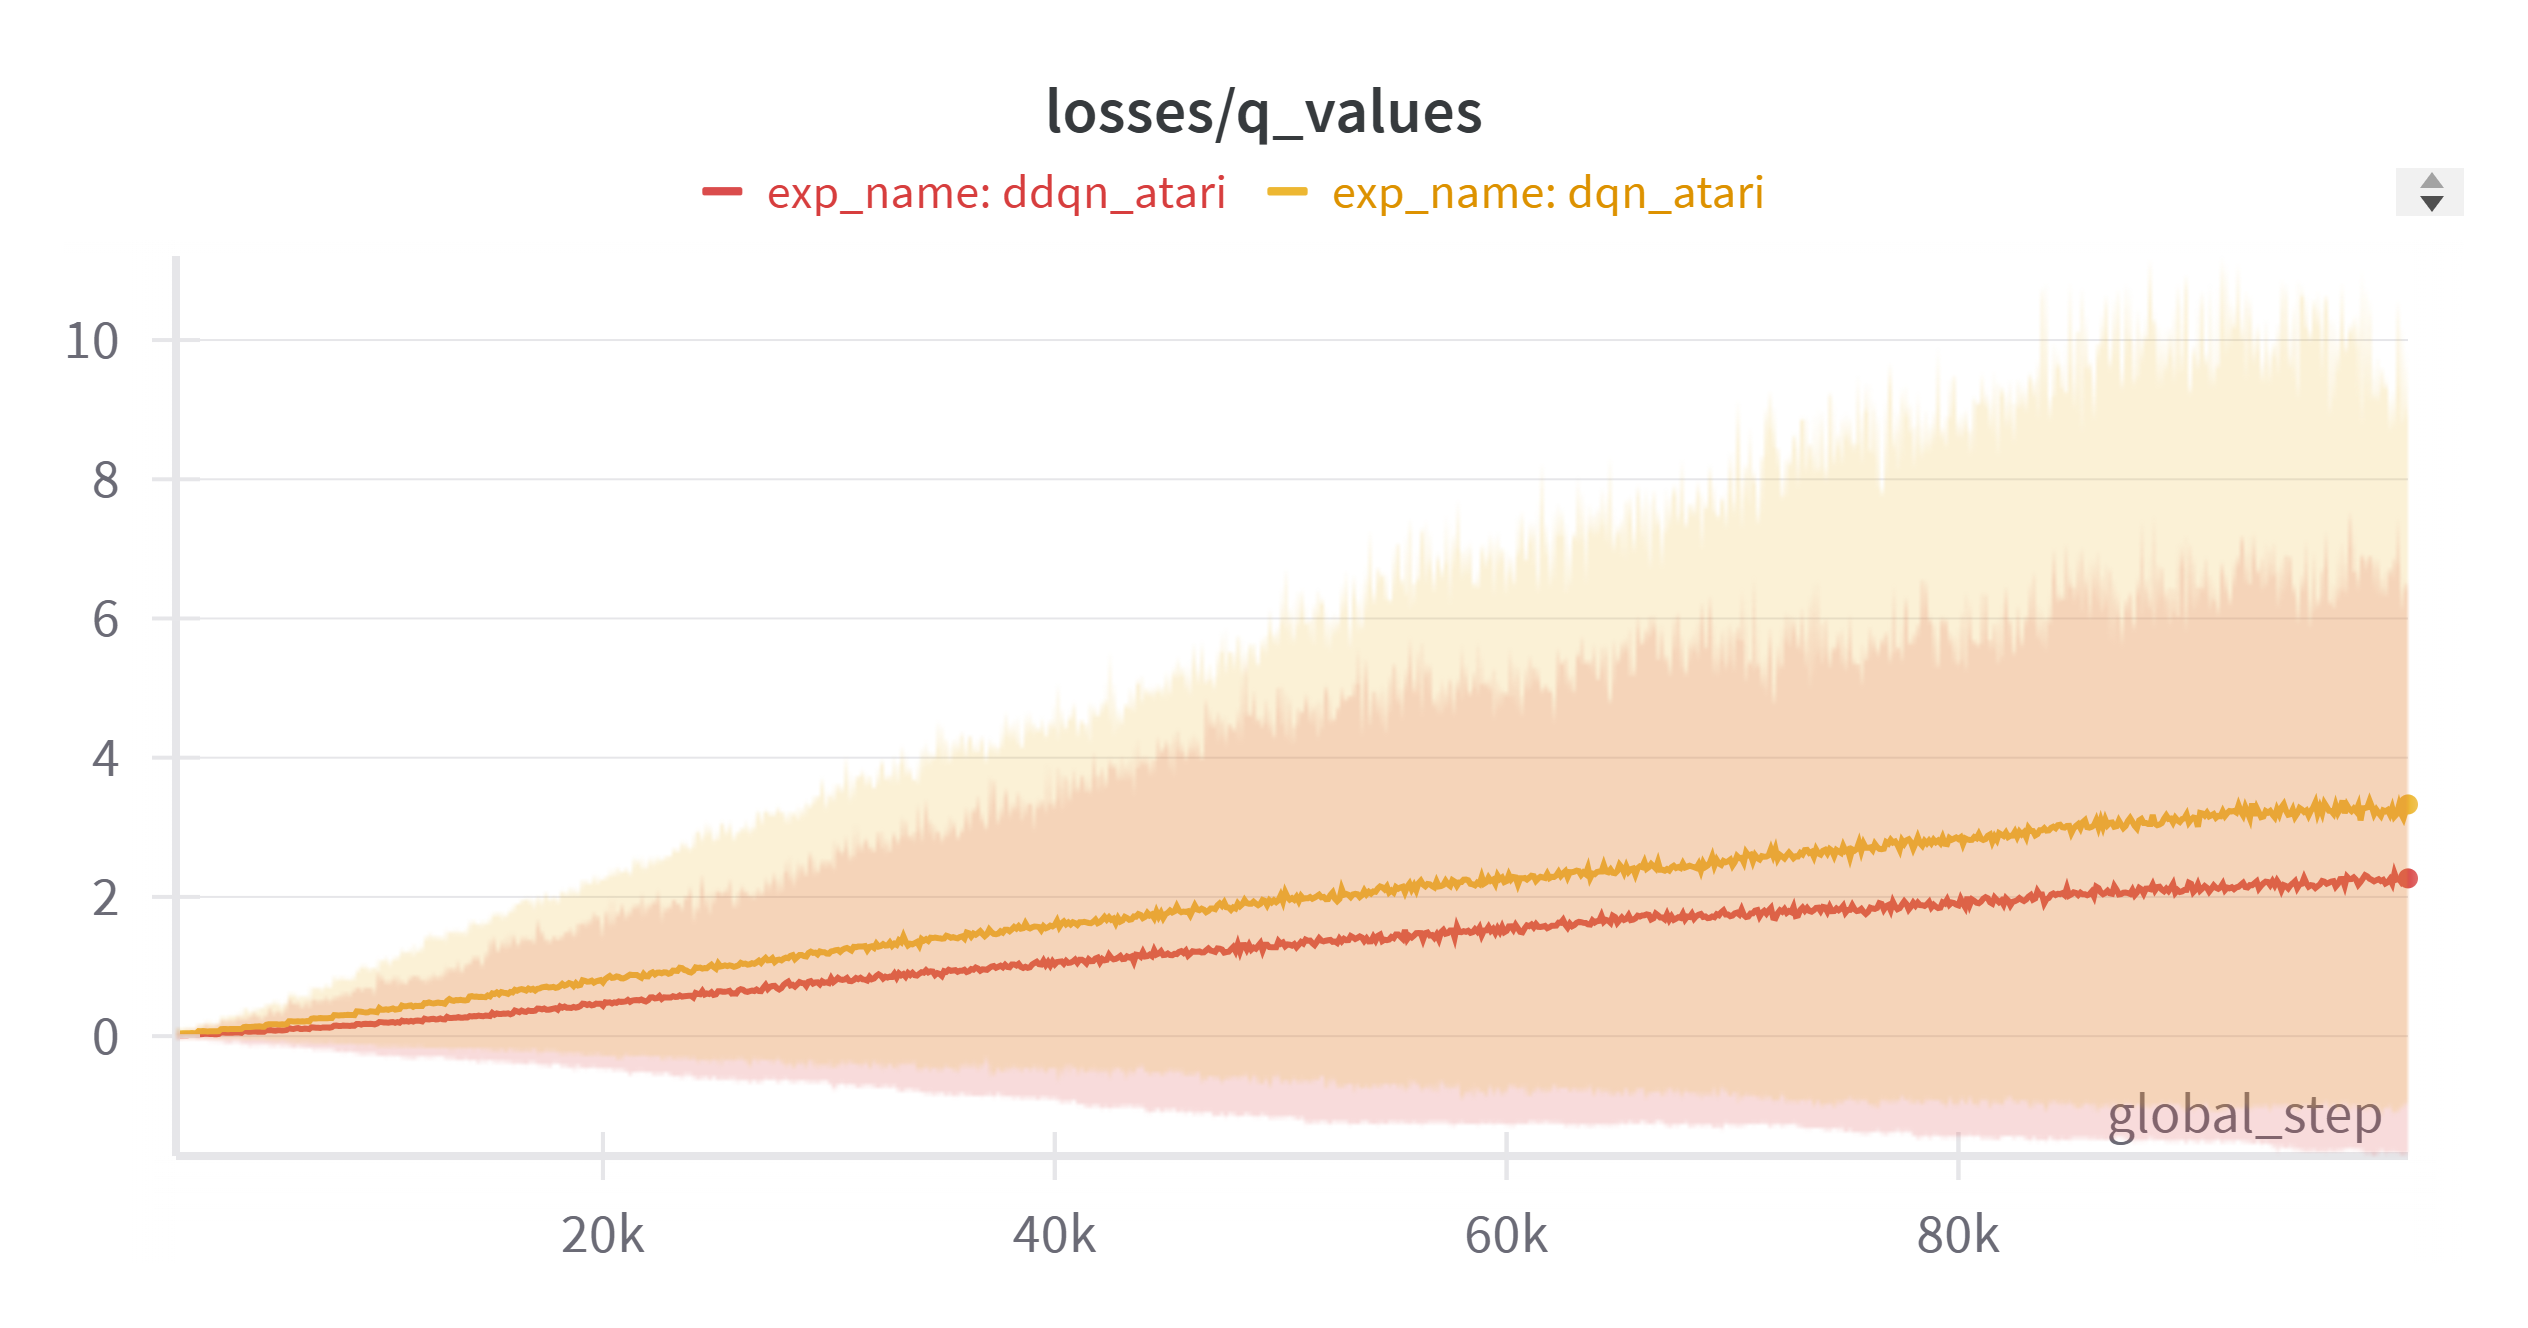
\includegraphics[width=0.6\textwidth]{figures/ddqn/png/comparison_losses_q_values_dqn_ddqn.png}
	\caption{Comparison of mean Q-values (with min--max shading) for DQN (gold) vs.\ Double DQN (red).}
	\label{fig:dqn_vs_ddqn_qvalues}
\end{figure}

\begin{figure}
	\centering
	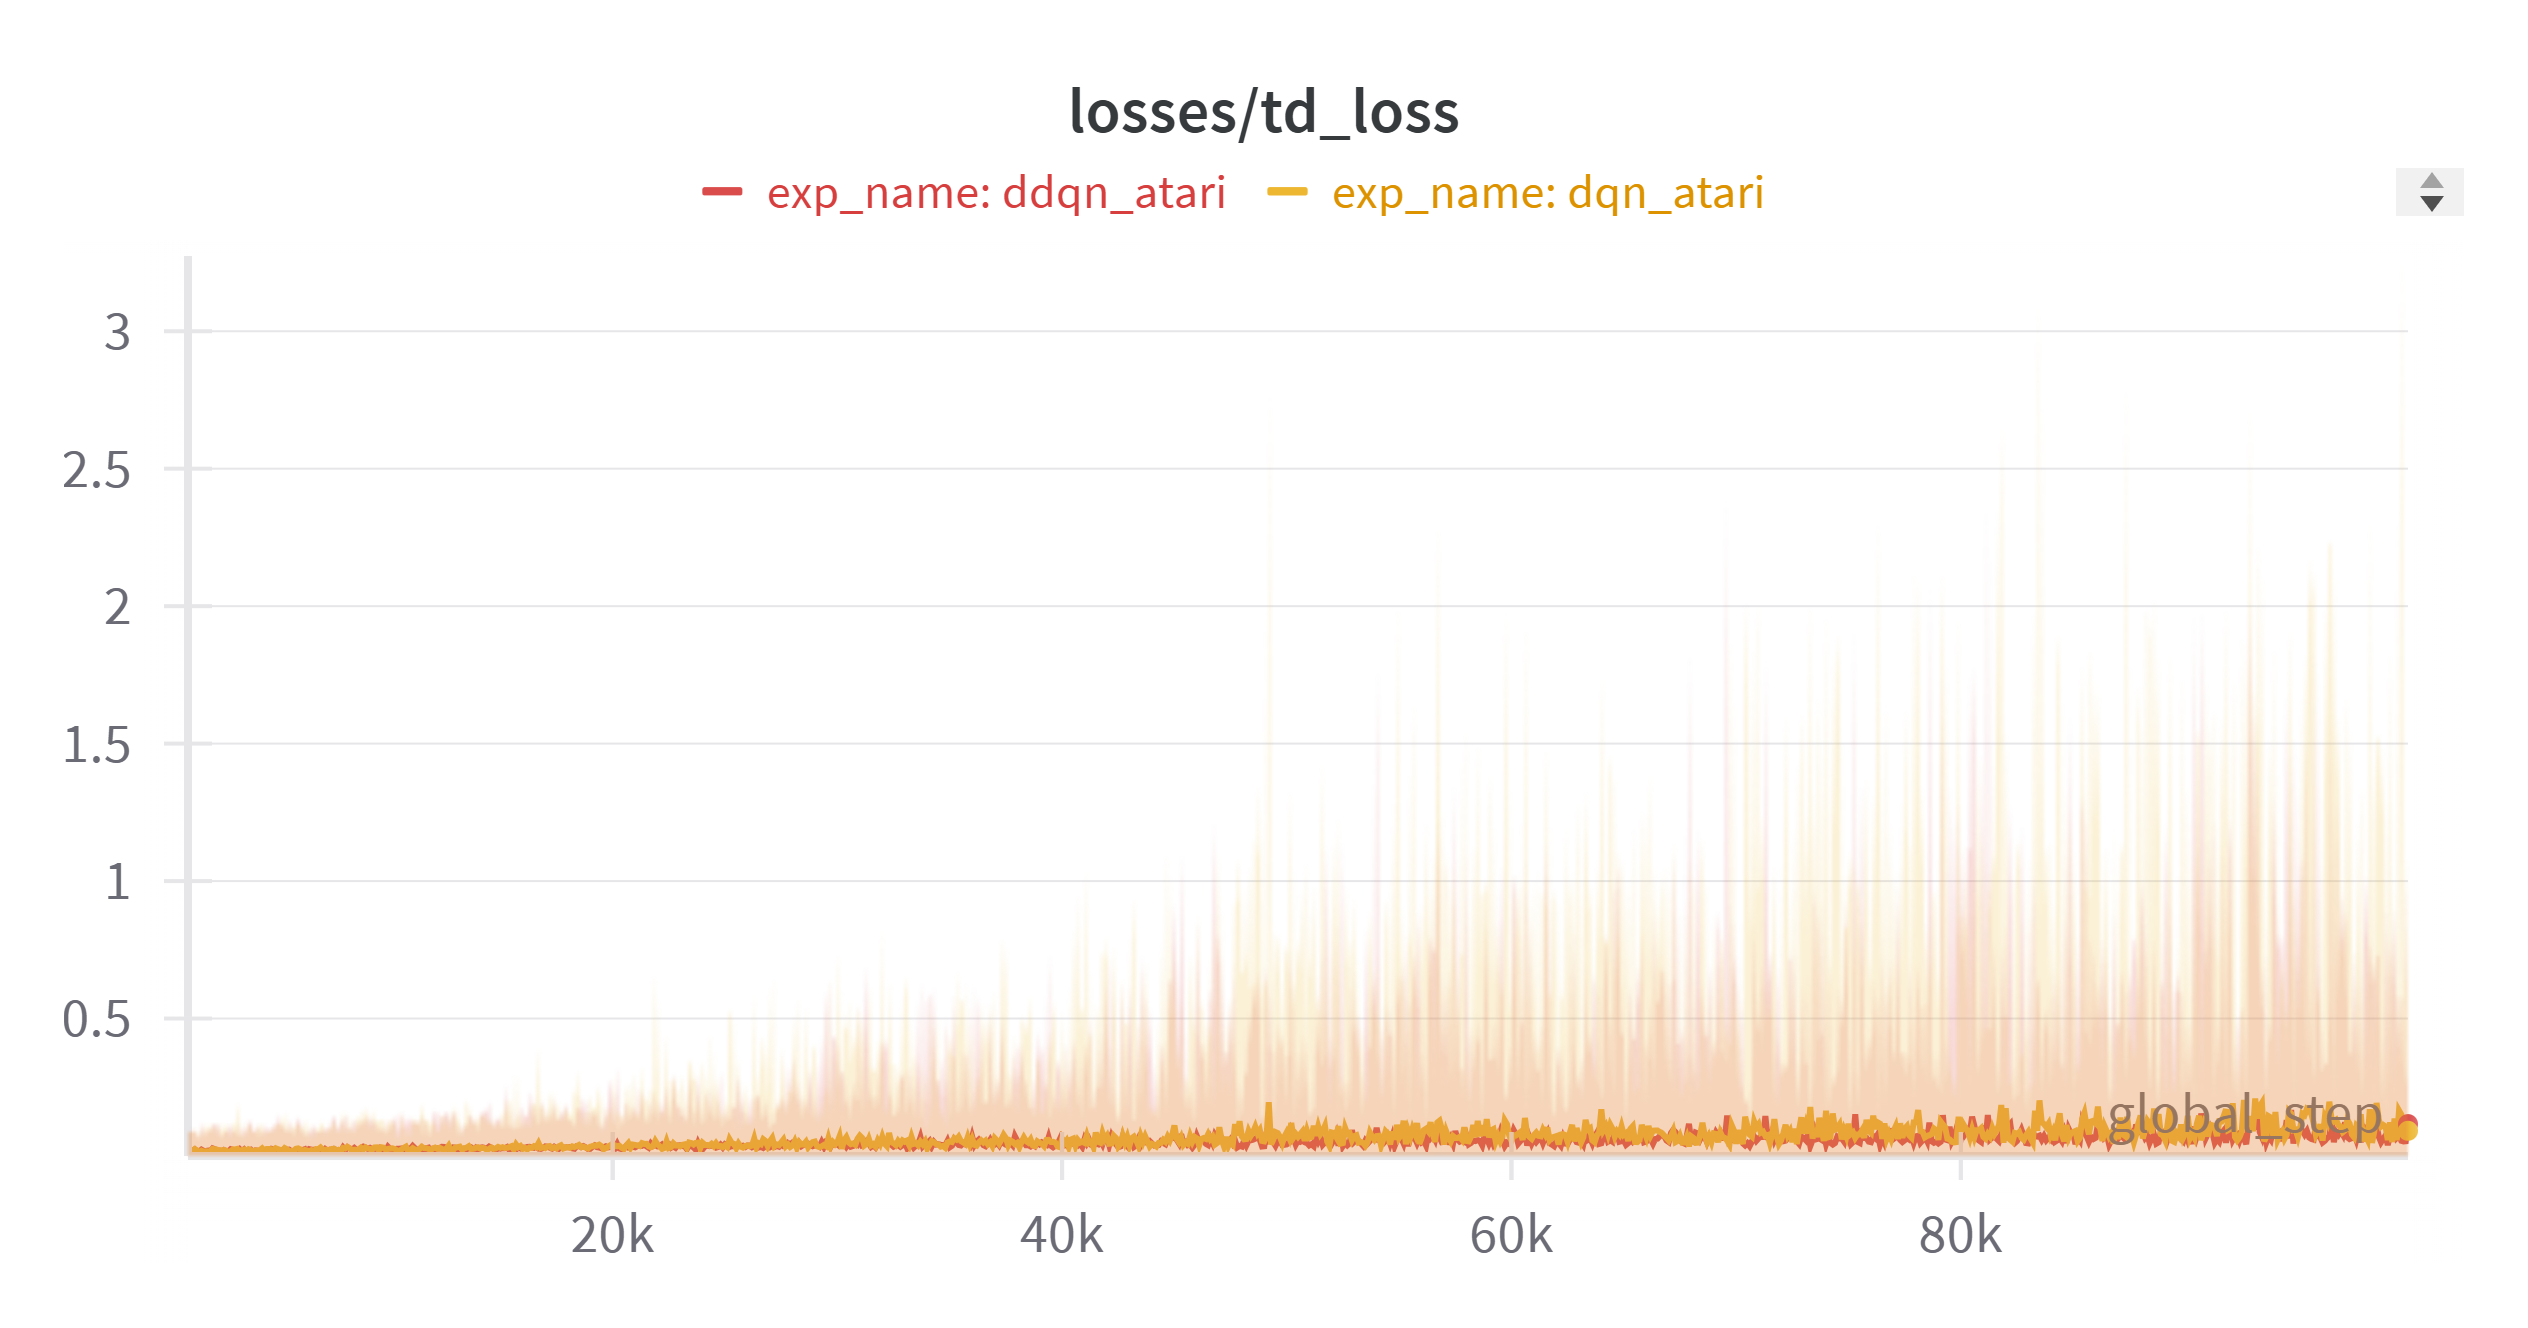
\includegraphics[width=0.6\textwidth]{figures/ddqn/png/comparison_losses_td_loss_dqn_ddqn.png}
	\caption{Comparison of TD loss for DQN (gold) vs.\ Double DQN (red). 
		Both remain near 0 for extended periods, though DQN shows slightly higher spikes.}
	\label{fig:dqn_vs_ddqn_td_loss}
\end{figure}


\begin{figure}
	\centering
	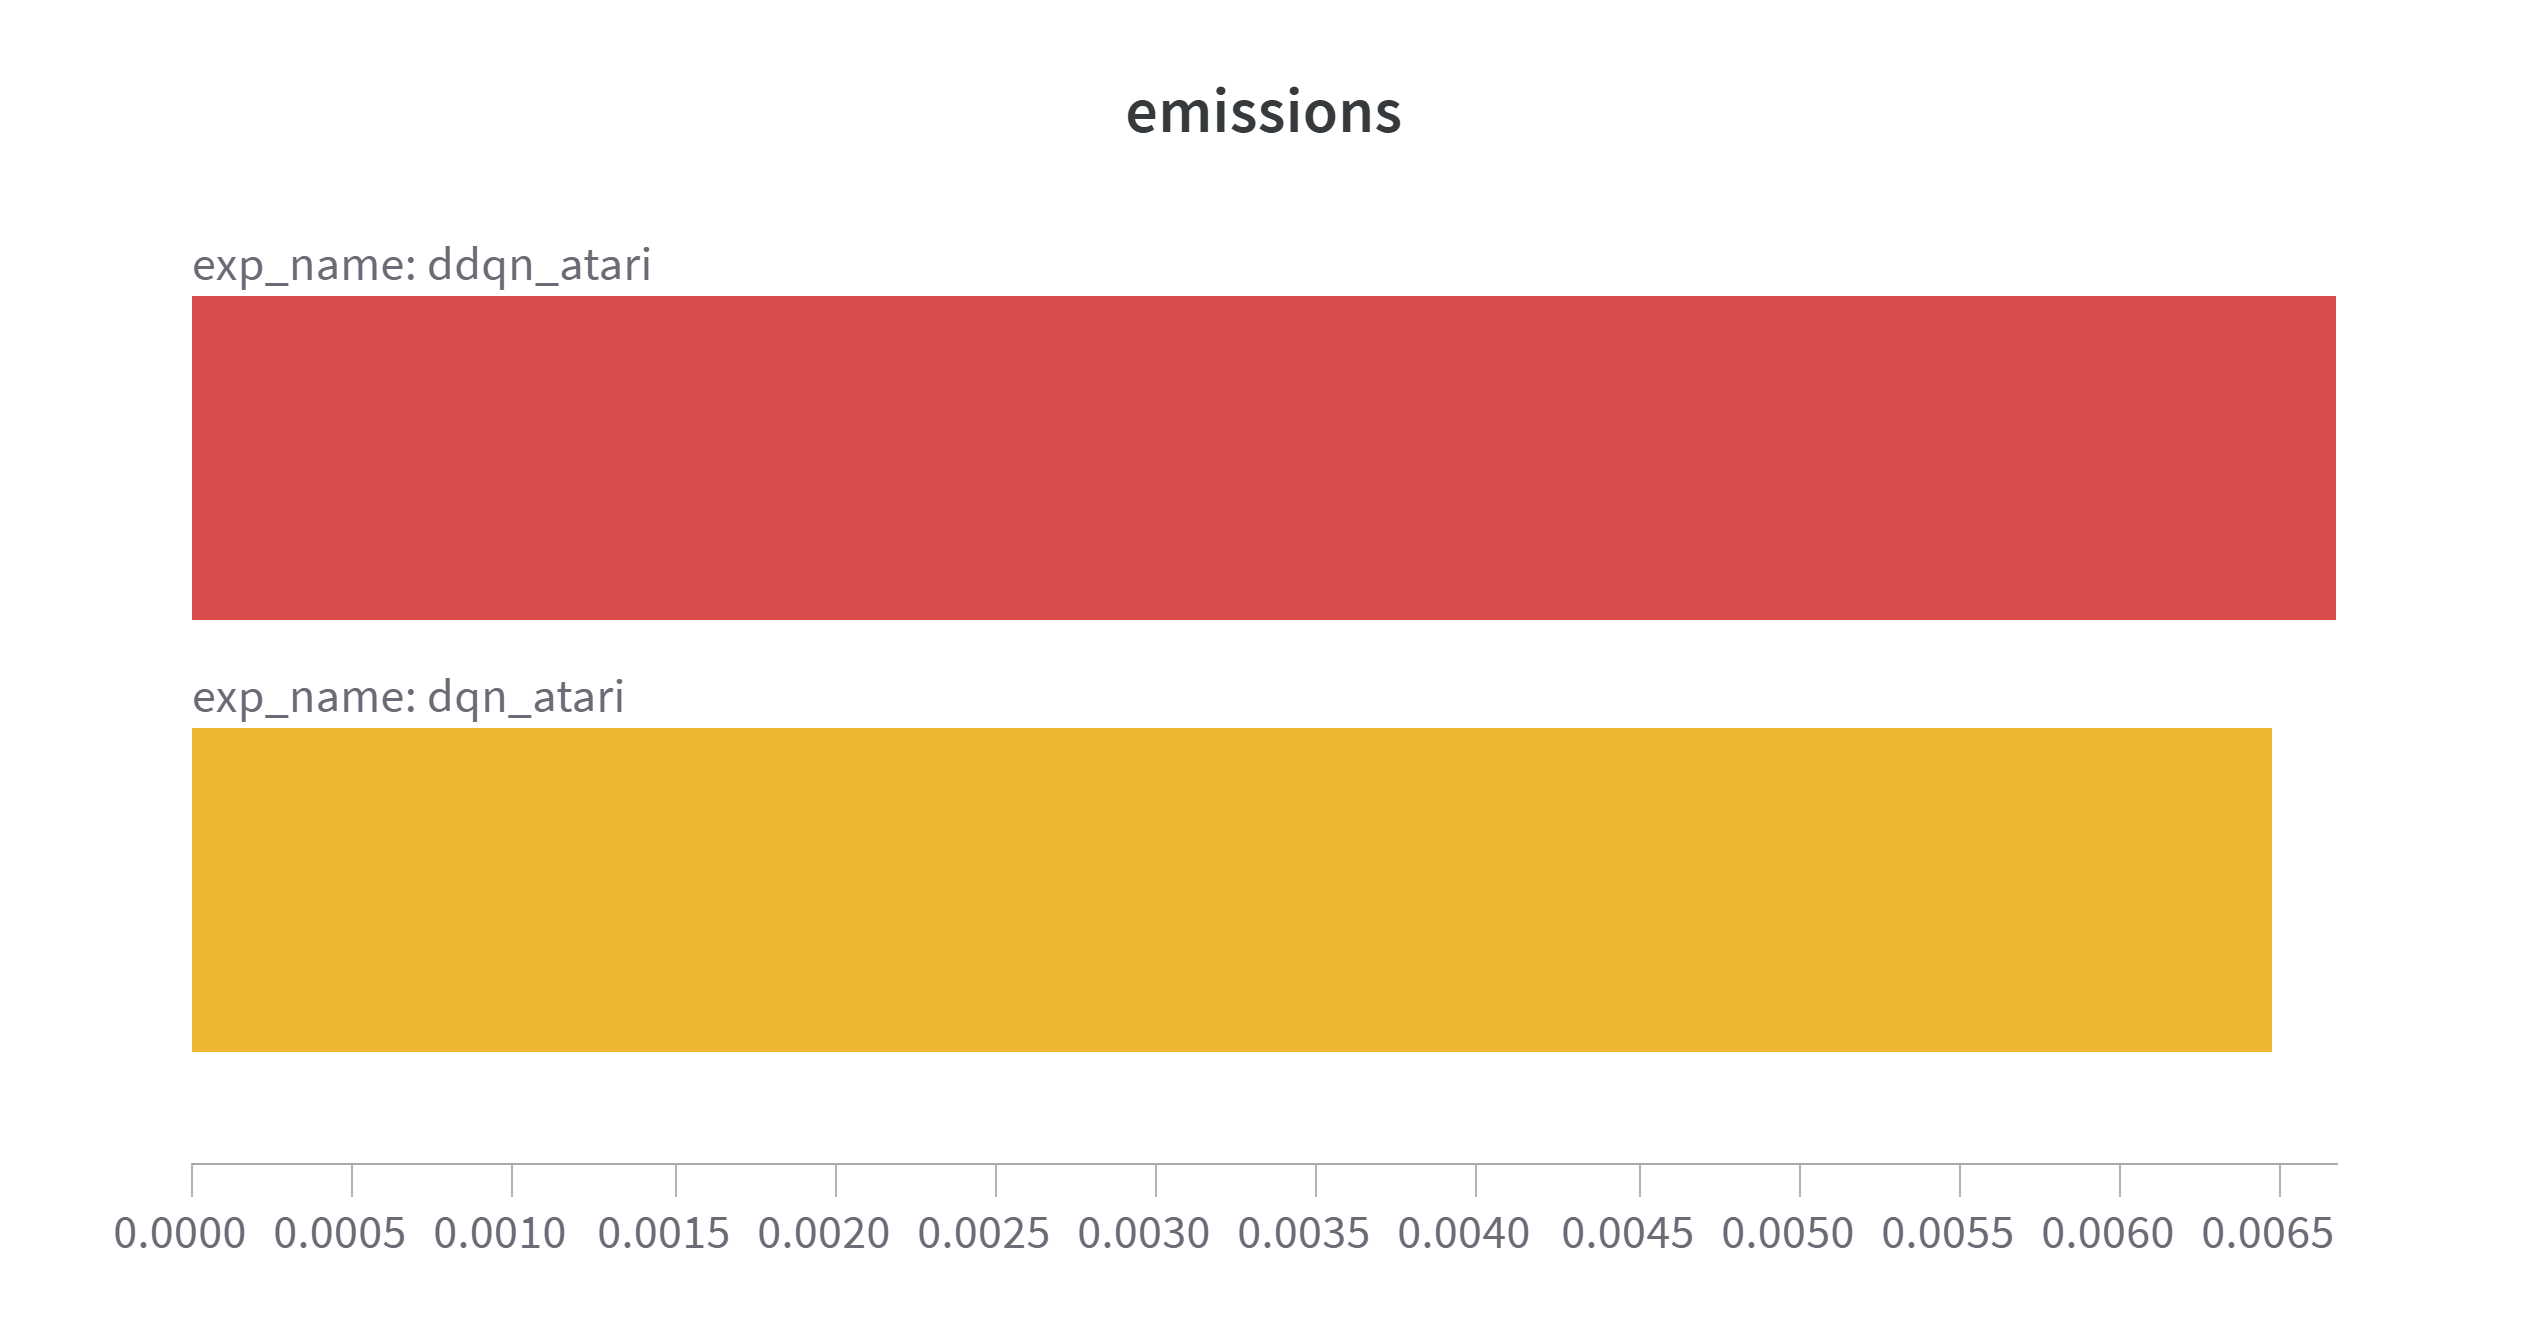
\includegraphics[width=0.6\textwidth]{figures/ddqn/png/emissions_dqn_ddqn.png}
	\caption{Mean emissions of DQN (gold) and Double DQN (red).}
	\label{fig:emissions_dqn_ddqn}
\end{figure}

Overall, Double DQN indeed moderates Q-value inflation compared to standard DQN, 
but under the 100k-step constraint, this reduction in overestimation does not strongly translate 
into consistently higher final returns.

\paragraph{Observations}
\begin{itemize}
	\item \textbf{Q-values and Losses:} Double DQN's Q-values peak lower than DQN's (about 2--3 vs.\ 4--5), aligning with the bias-reduction theory. TD losses remain small for both algorithms, with occasional spikes.
	\item \textbf{Performance:} The min--max normalized mean (\num{0.374}) is nearly the same as DQN's (\num{0.380}), while human-normalized is actually lower (\num{0.023} vs.\ \num{0.135}) due to certain highly negative runs, especially in \emph{Boxing}.
	\item \textbf{Emissions:} Average $\sim$\num{0.00667}\,kg\,CO\textsubscript{2}\,eq, slightly higher than DQN's \num{0.00647}\,kg.
\end{itemize}

Hence, although Double DQN successfully limits Q-value overestimation, its advantage does not 
fully manifest in higher aggregate returns at 100k steps—indicating that more extensive training 
or additional refinements may be needed to reap its potential performance gains.


\subsubsection{Prioritized Experience Replay (PER)}
\label{subsubsec:per}
In a standard DQN replay buffer, transitions are sampled \emph{uniformly}, giving equal 
probability to each experience. Prioritized Experience Replay (PER)~\cite{schaul:prioritized} 
seeks to allocate more sampling probability to transitions with higher TD error, 
on the premise that they contain more learning signal for the agent, thus achieving an effect
similar to that of prioritized sweeping in the value iteration algorithm for the tabular case.
With this focus on “informative” samples, also inspired by biology, PER can potentially
accelerate training and reduce sample complexity, especially in long training horizons.

The original paper proposes two primary methods to implement prioritization:
\begin{itemize}
	\item \textit{Sum-Tree} approach, which stores priority values $p_i$ in a binary tree, 
	allowing for efficient sampling of transitions proportional to $p_i^\alpha$.
	\item \textit{Rank-Based} approach, which sorts the buffer by TD error magnitude 
	and samples according to rank orders.
\end{itemize}
We adopt the \emph{sum-tree} variant in our implementation, 
mirroring the method described in \cite{schaul:prioritized} 
for improved efficiency over naive priority queues. 
Apart from this change, the underlying DQN hyperparameters 
(e.g., network architecture, target frequency) remain the same, 
and we incorporate importance-sampling corrections as recommended 
to offset the sampling bias introduced by prioritization.

We also explored two implementations of the PER replay buffer—a \texttt{numpy}-based (for consistency with the replay buffer used for the other algorithms) and a \texttt{torch}-based version. The \texttt{numpy} approach proved much slower, so we used the \texttt{torch} one in the final runs. It should be noted that even though the other DQN variants use a replay buffer numpy-based, it is the one implemented in Stable Baselines, so it employs optimizations that our version lacked. For this reason, we assume that using the torch-based implementation does not invalidate direct comparisons.

\paragraph{(Hyper)Parameters}
Table~\ref{tab:per_hyperparams} summarizes the key hyperparameters 
used in our PER implementation. 
Only \texttt{env\_id} and \texttt{seed} vary across runs 
(again, eight Atari games $\times$ four seeds = 32 runs), 
while other settings match those of the baseline DQN 
(Section~\ref{subsubsec:dqn_baseline}) to isolate PER's effects.

\begin{table}
	\caption{Key hyperparameters for Prioritized Experience Replay (PER). Only \texttt{env\_id} and \texttt{seed} vary across runs.}
	\label{tab:per_hyperparams}
	\centering
	\begin{tabular}{ll}
		\toprule
		\textbf{Parameter} & \textbf{Value} \\
		\midrule
		\texttt{exp\_name}                & per\_atari \\
		\texttt{seed}                     & 1..4 \\
		\texttt{torch\_deterministic}     & True \\
		\texttt{cuda}                     & True \\
		\texttt{track}                    & True \\
		\texttt{wandb\_project\_name}     & rlsb \\
		\texttt{capture\_video}           & False \\
		\texttt{save\_model}              & True \\
		\texttt{upload\_model}            & False \\
		\texttt{env\_id}                  & e.g.\ AmidarNoFrameskip-v4 \\
		\texttt{total\_timesteps}         & 100000 \\
		\texttt{learning\_rate}           & 0.0001 \\
		\texttt{num\_envs}                & 1 \\
		\texttt{buffer\_size}             & 10000 \\
		\texttt{gamma}                    & 0.99 \\
		\texttt{tau}                      & 1.0 \\
		\texttt{target\_network\_frequency} & 1000 \\
		\texttt{batch\_size}             & 32 \\
		\texttt{start\_e}, \texttt{end\_e} & 1.0 $\to$ 0.01 \\
		\texttt{exploration\_fraction}    & 0.1 \\
		\texttt{learning\_starts}         & 1000 \\
		\texttt{train\_frequency}         & 4 \\
		\bottomrule
	\end{tabular}
\end{table}

\paragraph{Hyperparameter Tuning}
We retained the same settings as baseline DQN (Section~\ref{subsubsec:dqn_baseline}) to highlight PER's impact alone, an approach mostly followed by the original authors too. Although \cite{schaul:prioritized} suggests lowering the learning rate by a factor of four, our tests at 100k steps with it and other values showed again that $1\times10^{-4}$ worked better. Figure~\ref{fig:per_lr_comparison} compares these rates on \emph{Breakout}, indicating faster convergence at $1\times10^{-4}$.  

\begin{figure}
	\centering
	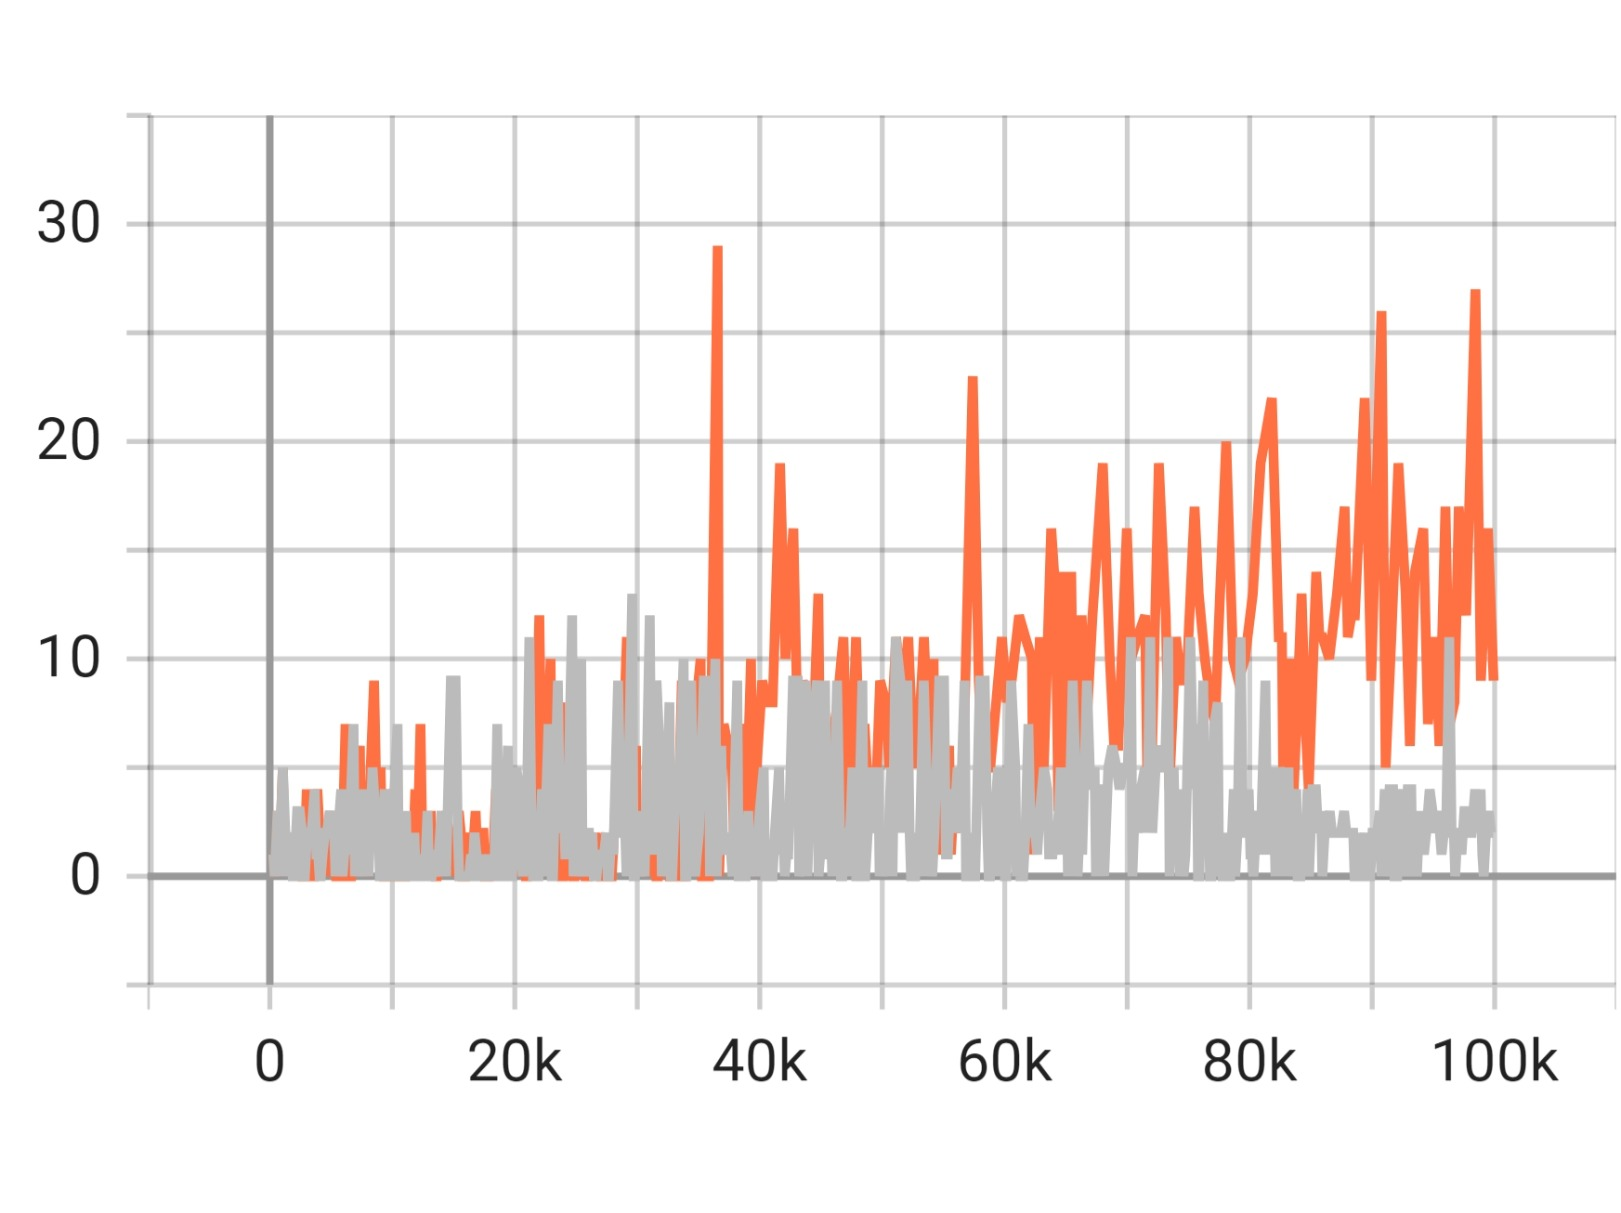
\includegraphics[width=0.55\textwidth]{figures/per/png/per_lr_charts_episodic_return.jpeg}
	\caption{Comparison of learning rates for PER on \emph{Breakout}. 
		Orange curve: $1\times10^{-4}$ (our final choice). 
		Gray curve: $\tfrac{1}{4}\times10^{-4}$ (as per \cite{schaul:prioritized}).}
	\label{fig:per_lr_comparison}
\end{figure}

\paragraph{Training Dynamics}
Figure~\vref{fig:per_training_metrics} aggregates four key metrics (episodic length, steps per second, Q-values, and TD loss) over 32 runs (eight games, four seeds each). PER shows Q-values approaching or exceeding those of baseline DQN (which typically topped at 4--5). The TD loss is small on average but spikes in certain runs, suggesting that prioritizing high-error samples can exacerbate updates in some episodes.

\begin{figure}
	\centering
	\subfloat[][\textit{Episodic length (\texttt{charts\_episodic\_length}). 
	The mean hovers around 3500--4000, and min--max runs from near 0 up to 8000.}]{
		\includesvg[width=.45\textwidth]{figures/per/charts_episodic_length_per_atari}
		\label{fig:per_episodic_length}
	}
	\quad
	\subfloat[][\textit{Steps per second (SPS). 
	The mean peaks above 170, then gradually declines to ~150--160.}]{
		\includesvg[width=.45\textwidth]{figures/per/charts_SPS_per_atari}
		\label{fig:per_sps}
	}
	\\[1em]
	\subfloat[][\textit{Q-values (\texttt{losses/q\_values}). 
	The mean eventually surpasses 4--5, with outliers above 14.}]{
		\includesvg[width=.45\textwidth]{figures/per/losses_q_values_per_atari}
		\label{fig:per_q_values}
	}
	\quad
	\subfloat[][\textit{TD loss (\texttt{losses/td\_loss}). 
	Some runs spike above 3--4, showing instability in late training.}]{
		\includesvg[width=.45\textwidth]{figures/per/losses_td_loss_per_atari}
		\label{fig:per_td_loss}
	}
	\caption{PER training metrics over 100k steps, interpolated across 32 runs.}
	\label{fig:per_training_metrics}
\end{figure}

\paragraph{Episodic Return}
Figures~\ref{fig:per_return_human} (human-normalized) and \ref{fig:per_return_minmax} (min--max) show PER's aggregated episodic returns. The mean in human-normalized scale oscillates around zero, occasionally dipping below $-2$ or $-3$ in some seeds.

\begin{figure}
	\centering
	\includesvg[width=0.6\textwidth]{figures/per/charts_episodic_return_human_per_atari}
	\caption{PER episodic return (human-normalized), aggregated over 32 runs. 
		Negative outliers appear for certain seeds/environments.}
	\label{fig:per_return_human}
\end{figure}

\begin{figure}
	\centering
	\includesvg[width=0.6\textwidth]{figures/per/charts_episodic_return_minmax_per_atari}
	\caption{PER episodic return (min--max normalized), aggregated over 32 runs.}
	\label{fig:per_return_minmax}
\end{figure}

\paragraph{Per-Game Returns}
Figures~\ref{fig:per_return_pergame_human} and \vref{fig:per_return_pergame_minmax} break down the performance by each Atari game (human vs. min--max normalization). We see, for instance, \emph{Freeway} (orange line in min--max) steadily climbing to around 0.7--0.8, while \emph{Alien} can drop below $-3$ in human scale. 

\begin{figure}
	\centering
	\includesvg[width=0.6\textwidth]{figures/per/charts_episodic_return_per_game_human_per_atari}
	\caption{PER returns per game (human-normalized). 
		\emph{Alien} (orange) exhibits deep negative dips, 
		while \emph{Freeway}, \emph{Assault}, and \emph{Breakout} stay near or above zero.}
	\label{fig:per_return_pergame_human}
\end{figure}

\begin{figure}
	\centering
	\includesvg[width=0.6\textwidth]{figures/per/charts_episodic_return_per_game_minmax_per_atari}
	\caption{PER returns per game (min--max normalized). 
		\emph{Freeway} (gold line) and \emph{Assault} (green) reach 0.7--0.8 near 100k steps.}
	\label{fig:per_return_pergame_minmax}
\end{figure}

\paragraph{Emissions.}
Table~\ref{tab:per_emissions} shows the statistics of the emissions of PER, while Figure~\vref{fig:per_vs_dqn_emissions} shows a barplot comparing PER's mean emissions ($\approx$ \num{0.00725}\,kg) to DQN's ($\approx$\num{0.00647}\,kg). The computational overhead of prioritized sampling may partly account for this higher footprint.

\begin{table}
	\caption{Carbon emissions (\si{\kilogram}\,CO\textsubscript{2}\,eq) for PER across 32 runs.}
	\label{tab:per_emissions}
	\centering
	\makebox[\textwidth]{%
	\begin{tabularx}{1.1\textwidth}{lXXXXXXXX}
		\toprule
		\textbf{Algorithm} & \textbf{mean} & \textbf{std} & \textbf{median} & \textbf{q25} & \textbf{q75} & \textbf{min} & \textbf{max} & \textbf{iqmean} \\
		\midrule
		PER & \num{0.007254} & \num{0.000263} & \num{0.007146} & \num{0.007074} & \num{0.007354} & \num{0.006935} & \num{0.007819} & \num{0.007157} \\
		\bottomrule
	\end{tabularx}
	}
\end{table}

\begin{figure}
	\centering
	\includesvg[width=0.55\textwidth]{figures/per/emissions_dqn_per}
	\caption{Mean emissions comparison: PER (green) at $\sim$\num{0.00725}\,kg vs.\ DQN (gold) at $\sim$\num{0.00647}\,kg.}
	\label{fig:per_vs_dqn_emissions}
\end{figure}

\begin{table}
	\caption{Overall final evaluation (10 episodes each) for PER across 32 runs.}
	\label{tab:per_eval_overall}
	\centering
	\makebox[\textwidth]{%
	\begin{tabular}{lcccccccc}
		\toprule
		\textbf{Normalization} & \textbf{mean} & \textbf{std} & \textbf{median} & 
		\textbf{q25} & \textbf{q75} & \textbf{min} & \textbf{max} & \textbf{iqmean} \\
		\midrule
		\textbf{Human}   & \num{0.0607} & \num{1.0170} & \num{0.0539} & \num{0.0175} & \num{0.2541} & \num{-10.2619} & \num{6.8809} & \num{0.0813} \\
		\textbf{Min--Max}& \num{0.3533} & \num{0.2695} & \num{0.2583} & \num{0.1499} & \num{0.6265} & \num{0.0} & \num{0.9845} & \num{0.3087} \\
		\bottomrule
	\end{tabular}
	}
\end{table}

\begin{table}
	\caption{Per-game final evaluation for PER (human- vs.\ min--max normalized). Each row aggregates 10 episodes $\times$ 4 seeds per environment.}
	\label{tab:per_eval_gamewise}
	\centering
	\begin{tabular}{llcccc}
		\toprule
		\textbf{Game} & \textbf{Norm} & \textbf{mean} & \textbf{std} & \textbf{min} & \textbf{max}\\
		\midrule
		Alien     & Human    & 0.0246 & 0.0315 & -0.0147 & 0.0996 \\
		& Min--Max & 0.0978 & 0.0523 & 0.0325  & 0.2225 \\
		\cmidrule{1-6}
		Amidar    & Human    & 0.0263 & 0.0220 & -0.0029 & 0.0809 \\
		& Min--Max & 0.2288 & 0.1693 & 0.0046  & 0.6498 \\
		\cmidrule{1-6}
		Assault   & Human    & 0.2135 & 0.0974 & 0.0232  & 0.3860 \\
		& Min--Max & 0.5648 & 0.1480 & 0.2757  & 0.8270 \\
		\cmidrule{1-6}
		Boxing    & Human    & -0.6667 & 2.7351 & -10.2619 & 6.8809 \\
		& Min--Max & 0.7388  & 0.0890 & 0.4264    & 0.9845 \\
		\cmidrule{1-6}
		Breakout  & Human    & 0.3854 & 0.2204 & 0.00997 & 0.9070 \\
		& Min--Max & 0.3500 & 0.1746 & 0.0526  & 0.7632 \\
		\cmidrule{1-6}
		Freeway   & Human    & 0.4071 & 0.3381 & 0.0     & 0.8446 \\
		& Min--Max & 0.4304 & 0.3574 & 0.0     & 0.8929 \\
		\cmidrule{1-6}
		MsPacman  & Human    & 0.0338 & 0.0111 & 0.0119 & 0.0515 \\
		& Min--Max & 0.2008 & 0.0446 & 0.1126 & 0.2723 \\
		\cmidrule{1-6}
		Pong      & Human    & 0.0617 & 0.0682 & -0.01 & 0.2233 \\
		& Min--Max & 0.2150 & 0.2045 & 0.0   & 0.7000 \\
		\bottomrule
	\end{tabular}
\end{table}

\paragraph{Comparison with Baseline DQN.}
By final evaluation, PER's overall human-norm mean (0.0607) is lower than DQN's (0.135), and its min--max mean (0.353) lags behind DQN's 0.380.  
Figure~\ref{fig:per_vs_dqn_emissions} further shows PER's emissions exceed DQN's by $\sim$\num{0.0008}\,kg\,CO\textsubscript{2}\,eq on average, likely due to the overhead from prioritized sampling and somewhat longer average episodes.

\paragraph{Observations.}
\begin{itemize}
	\item \textbf{Implementation Details:} 
	we used a \texttt{torch}-based PER buffer to avoid severe slowdowns in the \texttt{numpy} version.
	\item \textbf{Learning Rate:} 
	$\tfrac{1}{4}\times10^{-4}$, as suggested in \cite{schaul:prioritized}, underperformed at 100k steps 
	compared to $1\times10^{-4}$ (Figure~\vref{fig:per_lr_comparison}).
	\item \textbf{Performance:} 
	PER did not consistently outperform baseline DQN within 100k steps: 
	human-norm mean is \num{0.0607} vs.\ DQN's \num{0.135}. 
	\item \textbf{Emissions:} 
	PER's overhead leads to slightly higher energy usage (\num{0.00725}\,kg\,CO\textsubscript{2}\,eq) than DQN's \num{0.00647}\,kg.
\end{itemize}

In summary, while prioritizing high-error samples can yield benefits in longer training runs, 
our 100k-step Atari benchmark does not showcase a strong advantage. 
Further hyperparameter tuning or more extended runs might better reveal PER's strengths.


\subsubsection{Dueling DQN}
\label{subsubsec:dueling_dqn}
The \emph{Dueling DQN}~\cite{wang:dueling} architecture modifies the final layers of the Q-network
to separate the estimation of the state-value function $V(s)$ from that of the advantage function $A(s,a)$,
defined as $A(s, a) = Q(s, a) - V(s)$.
These two \textit{heads}, termed \textit{streams} in the paper, are then combined to yield
$$
Q(s, a) = V(s) + (A(s, a) - \mathcal{B})
$$
where $\mathcal{B}$ is a sort of "baseline" (see~\cite{wang:dueling} for the details on why this is necessary). The authors of the paper proposed either $\mathcal{B} = \max_{a' \in A(s)} A(s, a')$ or the \textit{average} $\mathcal{B} = \frac{1}{|\mathcal{A}|}\sum_{a' \in A(s)} A(s, a')$, but mainly experimented with the latter, so we did the same, as did most of the subsequent literature.

This approach allows the network to learn which states are valuable 
(\emph{regardless} of action) and which actions are relatively better than others 
(\emph{given} a state), thereby stabilizing learning in states where multiple actions have a close Q-value, and improving sample efficiency 
in many environments.

\paragraph{(Hyper)Parameters}
Adopting the same base configuration as our DQN baseline (Section~\ref{subsubsec:dqn_baseline}), we set 
\texttt{buffer\_size}=\num{10000} and \texttt{learning\_starts}=\num{1000} to accommodate the 100k-step regime. 
Table~\ref{tab:dueling_dqn_hyperparams} summarizes the key hyperparameters used in our Dueling DQN implementation. As with the baseline DQN, the \texttt{env\_id} and \texttt{seed} parameters were varied across runs to ensure statistically significant results across different games and random initializations.

Because the dueling architecture introduces separate streams for $V(s)$ and $A(s,a)$, the model ends up
with slightly more parameters than the baseline and other DQN variants. We considered reducing the size of the last shared layer to keep the
overall parameter count equal to the baseline, but being the difference only about 512 weights,
we opted to retain the original layer size for consistency with the other tested DQN variants.

The original Dueling DQN work introduced gradient clipping to maintain training stability, since there were now the gradients from two different stream
that merged into the common layers. However, our tests indicated no significant difference with or without its use, suggesting sufficient inherent stability in our setup. Therefore, we chose to omit it for consistency with the other algorithms implementations and to avoid introducing unnecessary modifications.

Finally, to maintain a controlled comparison, we did not combine dueling with Double DQN or PER (although that was explored in~\cite{wang:dueling}), as our primary goal is to evaluate the individual contribution of this single architectural tweak to performance and emissions, in line with our methodology for all DQN variants.

\begin{table}
	\caption{Key hyperparameters for Dueling DQN. Only \texttt{env\_id} and \texttt{seed} vary across runs.}
	\label{tab:dueling_dqn_hyperparams}
	\centering
	\begin{tabular}{ll}
		\toprule
		\textbf{Parameter} & \textbf{Value} \\
		\midrule
		\texttt{exp\_name}                & dueling\_dqn\_atari \\
		\texttt{seed}                     & 1..4 \\
		\texttt{torch\_deterministic}     & True \\
		\texttt{cuda}                     & True \\
		\texttt{track}                    & True \\
		\texttt{wandb\_project\_name}     & rlsb \\
		\texttt{capture\_video}           & False \\
		\texttt{save\_model}              & True \\
		\texttt{upload\_model}            & False \\
		\texttt{env\_id}                  & e.g.\ AlienNoFrameskip-v4 \\
		\texttt{total\_timesteps}         & 100000 \\
		\texttt{learning\_rate}           & 0.0001 \\
		\texttt{num\_envs}                & 1 \\
		\texttt{buffer\_size}             & 10000 \\
		\texttt{gamma}                    & 0.99 \\
		\texttt{tau}                      & 1.0 \\
		\texttt{target\_network\_frequency} & 1000 \\
		\texttt{batch\_size}             & 32 \\
		\texttt{start\_e}, \texttt{end\_e} & 1.0 $\to$ 0.01 \\
		\texttt{exploration\_fraction}    & 0.1 \\
		\texttt{learning\_starts}         & 1000 \\
		\texttt{train\_frequency}         & 4 \\
		\bottomrule
	\end{tabular}
\end{table}

\paragraph{Training Dynamics}
Figure~\ref{fig:dueling_training_metrics} displays key training metrics aggregated over 32 runs (8 games $\times$ 4 seeds). 

As shown in Figure~\ref{fig:dueling_episodic_length}, the episodic length generally hovers between 3500 and 4000 steps, exhibiting variability with minimums near 0 and maximums reaching up to 8000. The steps-per-second (SPS) metric, depicted in Figure~\ref{fig:dueling_sps}, shows an initial ramp-up phase before stabilizing around 155-160, slightly below the baseline DQN's average of approximately 165-170.

Q-values (Figure~\ref{fig:dueling_q_values}) generally ascend beyond 4-5, with some outliers reaching 8-10, a trend consistent with standard DQN but with slightly lower peak values than Double DQN or PER. 

The TD loss (Figure~\ref{fig:dueling_td_loss}) remains relatively low, generally staying below 1.5-2.0, with some runs exhibiting increased variability later in training. 

\begin{figure}
	\centering
	\subfloat[][\textit{Episodic length. 
	The mean hovers around 3500--4000 steps, with min--max from near 0 up to 8000.}]{
		\includesvg[width=.45\textwidth]{figures/dueling_dqn/charts_episodic_length_dueling_dqn_atari}
		\label{fig:dueling_episodic_length}
	}
	\quad
	\subfloat[][\textit{Steps per second (SPS). 
	After an initial ramp-up near 170, it stabilizes around 155--160.}]{
		\includesvg[width=.45\textwidth]{figures/dueling_dqn/charts_SPS_dueling_dqn_atari}
		\label{fig:dueling_sps}
	}
	\\[1em]
	\subfloat[][\textit{Q-values (\texttt{losses/q\_values}). 
	The mean grows beyond 4--5, with outliers near 8--10.}]{
		\includesvg[width=.45\textwidth]{figures/dueling_dqn/losses_q_values_dueling_dqn_atari}
		\label{fig:dueling_q_values}
	}
	\quad
	\subfloat[][\textit{TD loss (\texttt{losses/td\_loss}). 
	Some runs spike above 1.5--2.0, showing moderate variability late in training.}]{
		\includesvg[width=.45\textwidth]{figures/dueling_dqn/losses_td_loss_dueling_dqn_atari}
		\label{fig:dueling_td_loss}
	}
	\caption{Dueling DQN training metrics over 100k steps, aggregated over 32 runs.}
	\label{fig:dueling_training_metrics}
\end{figure}

\paragraph{Episodic Return (Aggregated)}
Figures~\ref{fig:dueling_return_human} and~\ref{fig:dueling_return_minmax} show 
the average episodic returns over 100k steps, in \emph{human-normalized} and 
\emph{min--max normalized} scales, respectively. 

As seen in  Figure~\ref{fig:dueling_return_human}, the human-normalized returns exhibit significant variance, with occasional dips below -8. The mean trend hovers around 0.1-0.2, slightly surpassing the baseline DQN's typical value, but is influenced by the volatility of results in environments like \emph{Boxing}.

Min-Max Normalized curve, in (Fig.~\ref{fig:dueling_return_minmax}) scales near 0.1-0.2 to 0.35-0.45, which equals to what see for the baseline implementation.

\begin{figure}
	\centering
	\includesvg[width=0.6\textwidth]{figures/dueling_dqn/charts_episodic_return_human_dueling_dqn_atari}
	\caption{Dueling DQN episodic return (human-normalized) over 100k steps. 
		Variance is significant, with some dips below -8.}
	\label{fig:dueling_return_human}
\end{figure}

\begin{figure}
	\centering
	\includesvg[width=0.6\textwidth]{figures/dueling_dqn/charts_episodic_return_minmax_dueling_dqn_atari}
	\caption{Dueling DQN episodic return (min--max normalized) aggregated over 32 runs.}
	\label{fig:dueling_return_minmax}
\end{figure}

\paragraph{Per-Game Returns}
Figures~\ref{fig:dueling_return_pergame_human} and~\ref{fig:dueling_return_pergame_minmax} 
provide a detailed breakdown of returns for each of the 8 Atari games:
On Figure~\ref{fig:dueling_return_pergame_human}, with the human normalized metrics, you can see that \emph{Boxing} (orange) can swing from $-1.93$ up to $+3.55$, while \emph{Freeway} and \emph{Assault} can reach higher normalized scores.
Figure~\ref{fig:dueling_return_pergame_minmax} demonstrates that, considering the min--max normalization, \emph{Freeway} often pushes above 0.7, \emph{Assault} similarly reaches 0.7--0.8.

\begin{figure}
	\centering
	\includesvg[width=0.6\textwidth]{figures/dueling_dqn/charts_episodic_return_per_game_human_dueling_dqn_atari}
	\caption{Dueling DQN returns per game (human-normalized). 
		\emph{Boxing} (orange) experiences deep negative dips, while \emph{Freeway} and \emph{Assault} can reach higher normalized scores.}
	\label{fig:dueling_return_pergame_human}
\end{figure}

\begin{figure}
	\centering
	\includesvg[width=0.6\textwidth]{figures/dueling_dqn/charts_episodic_return_per_game_minmax_dueling_dqn_atari}
	\caption{Dueling DQN returns per game (min--max normalized). 
		\emph{Freeway} (gold) and \emph{Assault} (green) often exceed 0.7.}
	\label{fig:dueling_return_pergame_minmax}
\end{figure}

\paragraph{Emissions}
Table~\ref{tab:dueling_dqn_emissions} presents the aggregated carbon footprint: 
a mean of \num{0.006893}\,kg\,CO\textsubscript{2}\,eq, with a standard deviation of \num{0.00029}. 
This is higher than the baseline DQN's $\sim$\num{0.00647}\,kg 
but still below some others (e.g., PER's $\sim$\num{0.00725}\,kg). 
Figure~\ref{fig:dueling_emissions_barplot} illustrates a direct comparison 
between Dueling DQN and baseline DQN.

\begin{table}
	\caption{Carbon emissions (kg\,CO\textsubscript{2}\,eq) for Dueling DQN across 32 runs.}
	\label{tab:dueling_dqn_emissions}
	\centering
	\makebox[\textwidth]{%
	\begin{tabular}{lcccccccc}
		\toprule
		\textbf{Algorithm} & \textbf{mean} & \textbf{std} & \textbf{median} & 
		\textbf{q25} & \textbf{q75} & \textbf{min} & \textbf{max} & \textbf{iqmean} \\
		\midrule
		Dueling DQN & 0.006893 & 0.0002901 & 0.006742 & 0.006672 & 0.007002 & 0.006617 & 0.007478 & 0.006779 \\
		\bottomrule
	\end{tabular}
	}
\end{table}

\begin{figure}
	\centering
	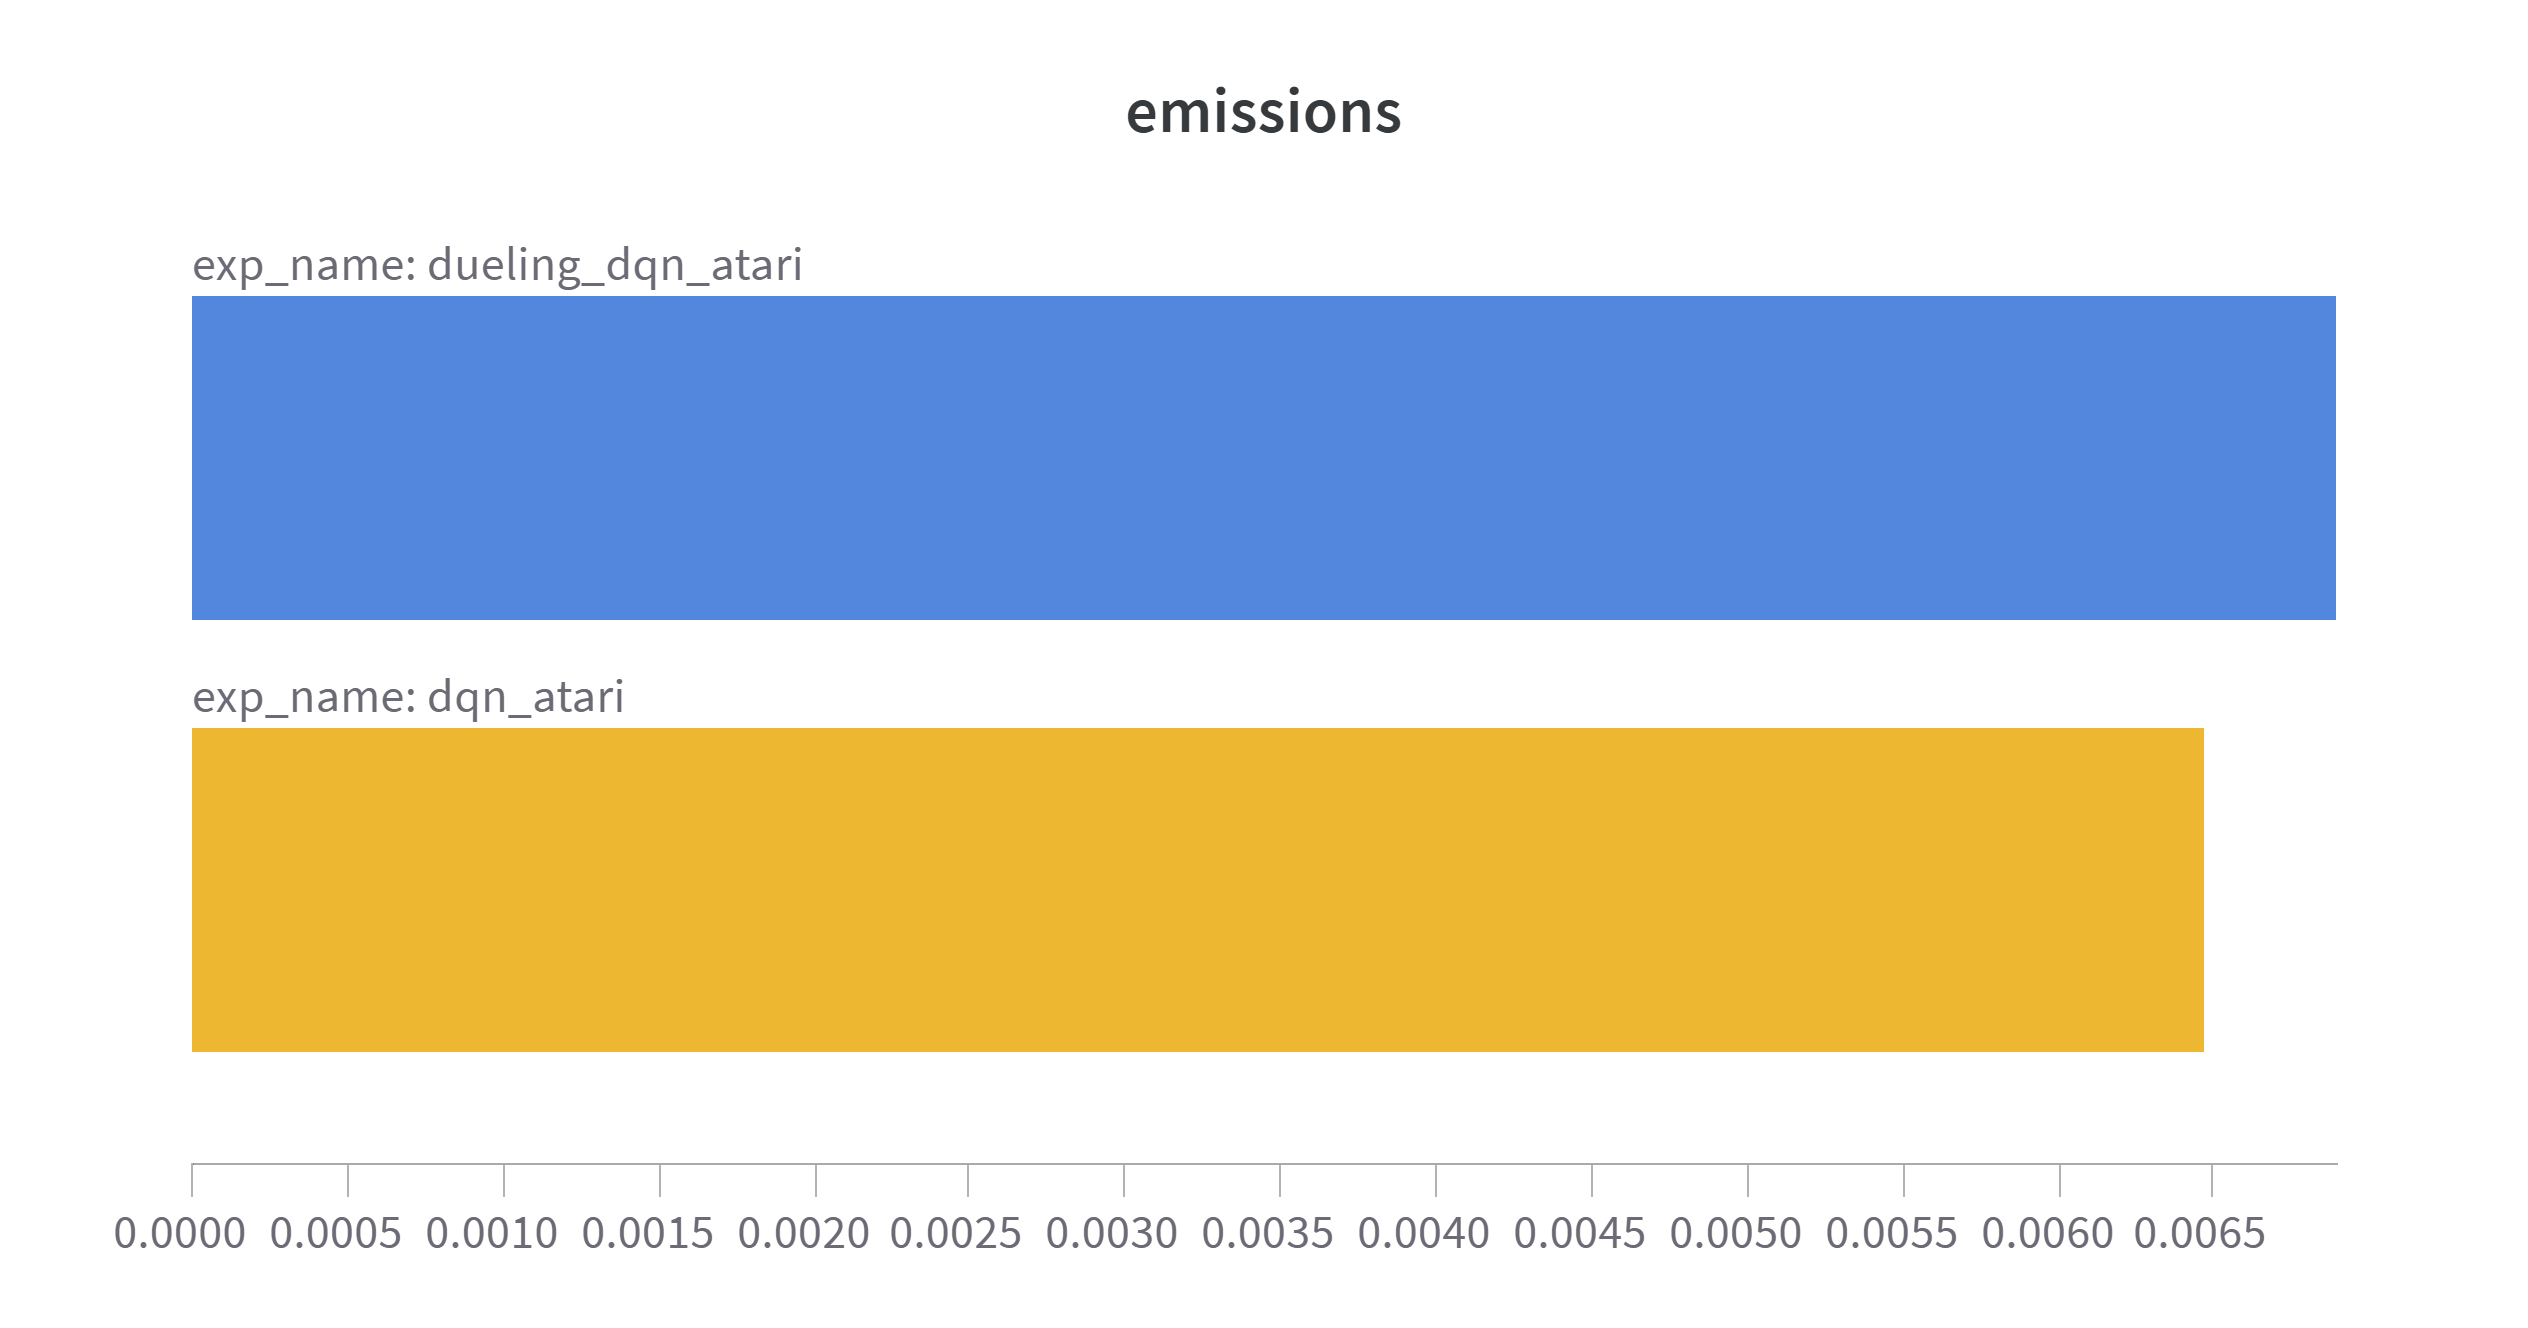
\includegraphics[width=0.55\textwidth]{figures/dueling_dqn/png/emissions_dqn_dueling.png}
	\caption{Mean emissions comparison: Dueling DQN (blue) at $\sim$\num{0.00689}\,kg vs.\ DQN (gold) at $\sim$\num{0.00647}\,kg.}
	\label{fig:dueling_emissions_barplot}
\end{figure}

\paragraph{Evaluation Results}
Table~\ref{tab:dueling_dqn_eval_overall} reports the overall final evaluation (10 episodes each) for Dueling DQN across all 32 runs, while Table~\ref{tab:dueling_dqn_eval_gamewise} provides a game-by-game breakdown.
Analyzing these results, we observe that in the human-normalized version, the Dueling DQN performance on Freeway is lower than that of DQN and Double DQN (which achieve values around 0.7), with the lower score for Boxing pulling down the overall average. In contrast, the min–max normalized values are in line with similar algorithms, with Freeway consistently showing the best performance.

\begin{table}
	\caption{Overall final evaluation (10 episodes each) for Dueling DQN across 32 runs.}
	\label{tab:dueling_dqn_eval_overall}
	\centering
	\makebox[\textwidth]{%
	\begin{tabular}{lcccccccc}
		\toprule
		\textbf{Normalization} & \textbf{mean} & \textbf{std} & \textbf{median} & 
		\textbf{q25} & \textbf{q75} & \textbf{min} & \textbf{max} & \textbf{iqmean} \\
		\midrule
		\textbf{Human}   & 0.1860 & 0.5258 & 0.0402 & 0.0148 & 0.3530 & -1.9286 & 3.5476 & 0.1020 \\
		\textbf{Min--Max}& 0.3849 & 0.3056 & 0.2632 & 0.1100 & 0.7448 & 0.0 & 0.9523 & 0.3454 \\
		\bottomrule
	\end{tabular}
	}
\end{table}

\begin{table}
	\caption{Per-game final evaluation for Dueling DQN (human- vs.\ min--max normalized).}
	\label{tab:dueling_dqn_eval_gamewise}
	\centering
	\begin{tabular}{llcccc}
		\toprule
		\textbf{Game} & \textbf{Norm} & \textbf{mean} & \textbf{std} & \textbf{min} & \textbf{max}\\
		\midrule
		Alien     & Human    & 0.0398 & 0.0346 & -0.0072 & 0.1493 \\
		& Min--Max & 0.1231 & 0.0574 & 0.0450  & 0.3050 \\
		\cmidrule{1-6}
		Amidar    & Human    & 0.0372 & 0.0193 & 0.0235 & 0.0935 \\
		& Min--Max & 0.3127 & 0.1482 & 0.2074 & 0.7465 \\
		\cmidrule{1-6}
		Assault   & Human    & 0.3200 & 0.0985 & 0.1057 & 0.4684 \\
		& Min--Max & 0.7266 & 0.1498 & 0.4010 & 0.9523 \\
		\cmidrule{1-6}
		Boxing    & Human    & 0.1190 & 1.3282 & -1.9286 & 3.5476 \\
		& Min--Max & 0.7643 & 0.0432 & 0.6977  & 0.8760 \\
		\cmidrule{1-6}
		Breakout  & Human    & 0.4020 & 0.2904 & -0.0565 & 1.0066 \\
		& Min--Max & 0.3632 & 0.2300 & 0.0     & 0.8421 \\
		\cmidrule{1-6}
		Freeway   & Human    & 0.5372 & 0.3162 & 0.0     & 0.7770 \\
		& Min--Max & 0.5679 & 0.3342 & 0.0     & 0.8214 \\
		\cmidrule{1-6}
		MsPacman  & Human    & 0.0265 & 0.0204 & 0.00018 & 0.0736 \\
		& Min--Max & 0.1713 & 0.0823 & 0.0654  & 0.3613 \\
		\cmidrule{1-6}
		Pong      & Human    & 0.0067 & 0.0185 & -0.01 & 0.0567 \\
		& Min--Max & 0.0500 & 0.0555 & 0.0   & 0.2 \\
		\bottomrule
	\end{tabular}
\end{table}

\paragraph{Comparison with Baseline DQN}
In final evaluation, Dueling DQN's \emph{human}-norm mean is \num{0.1860} vs.\ DQN's \num{0.1353}, 
and the \emph{min--max} mean is \num{0.3849} vs.\ DQN's \num{0.3802}—so we see a small positive difference on average.
However, \emph{Boxing} outliers (some runs exceed 3.5, others dip below $-1.9$) inflate the variance.
Meanwhile, emissions at $\sim$\num{0.00689}\,kg\,CO\textsubscript{2}\,eq are higher than DQN's $\sim$\num{0.00647} but remain
lower than some other variants (e.g.\ PER at \num{0.00725}).

\paragraph{Observations}
\begin{itemize}
	\item \textbf{Architecture Impact:}
	The \emph{dueling} approach separates state-value and advantage,
	intending to stabilize updates in states where action choices matter less.
	\item \textbf{Network Size:}
	We kept the same shared layer size as DQN, adding only a modest number of extra parameters.
	\item \textbf{Performance:}
	The final mean in human normalization (0.1860) is higher than baseline DQN's 0.1353,
	though min--max (0.3849 vs.\ 0.3802) is only slightly larger.
	\item \textbf{Emissions:}
	Dueling DQN uses $\sim$\num{0.00689}\,kg\,CO\textsubscript{2}\,eq,
	more than DQN's 0.00647 but less than PER's 0.00725.
\end{itemize}

Overall, Dueling DQN yields a small performance boost compared to baseline DQN 
within 100k steps, at a marginally higher carbon cost, consistent with the idea 
that decoupling $V(s)$ from $A(s,a)$ can help focus updates in states 
where actions yield similar Q-values.

\subsubsection{Categorical DQN (C51)}
\label{subsubsec:c51}
Categorical DQN (C51)~\cite{bellemare:distributional} extends the traditional DQN framework by modeling the action-value function $Q(s,a)$ as a full (discrete) probability distribution over possible returns rather than just a single expected value. This distributional approach enables the agent to capture not only the mean reward but also the variability and uncertainty associated with future returns. C51 achieves this by discretizing the range of potential returns, spanning from $v_{\mathrm{min}}$ to $v_{\mathrm{max}}$, into a fixed set of support points (atoms).

During the learning process, the algorithm projects the Bellman update onto this discrete support and uses a cross-entropy loss to align the predicted distribution with the target distribution. Such a rich representation of returns is particularly beneficial in risk-sensitive or high-variance environments, as it provides more informative learning signals that can lead to improved stability and performance over longer training periods. Although this enhanced representation introduces additional computational overhead, as reflected by the increased emissions compared to the baseline DQN, it holds promise for more nuanced decision-making in complex tasks.

\paragraph{(Hyper)Parameters}
The key hyperparameters used for the C51 implementation are summarized in Table~\ref{tab:c51_hyperparams}. In this configuration, most settings remain constant across runs, with only the environment identifier (\texttt{env\_id}) and the random seed (\texttt{seed}) varying. Notably, C51 employs a discrete return distribution with 51 atoms spanning the interval $[-10, 10]$, and uses a learning rate of \num{0.00025}. Other parameters such as the total timesteps (\num{100000}), batch size (32), and target network update frequency (\num{1000}) have been kept consistent with the other tested algorithm. 

\begin{table}
	\caption{Key hyperparameters for the C51 algorithm. Only \texttt{env\_id} and \texttt{seed} vary across runs.}
	\label{tab:c51_hyperparams}
	\centering
	\begin{tabular}{ll}
		\toprule
		\textbf{Parameter} & \textbf{Value} \\
		\midrule
		\texttt{exp\_name}                & c51\_atari \\
		\texttt{seed}                     & 1..4 \\
		\texttt{torch\_deterministic}     & True \\
		\texttt{cuda}                     & True \\
		\texttt{track}                    & True \\
		\texttt{wandb\_project\_name}     & rlsb \\
		\texttt{capture\_video}           & False \\
		\texttt{save\_model}              & True \\
		\texttt{upload\_model}            & False \\
		\texttt{env\_id}                  & e.g.\ AlienNoFrameskip-v4 \\
		\texttt{total\_timesteps}         & 100000 \\
		\texttt{learning\_rate}           & 0.00025 \\
		\texttt{num\_envs}                & 1 \\
		\texttt{n\_atoms}                 & 51 \\
		\texttt{v\_min}                   & -10 \\
		\texttt{v\_max}                   & 10 \\
		\texttt{buffer\_size}             & 10000 \\
		\texttt{gamma}                    & 0.99 \\
		\texttt{target\_network\_frequency} & 1000 \\
		\texttt{batch\_size}             & 32 \\
		\texttt{start\_e}, \texttt{end\_e} & 1.0 $\to$ 0.01 \\
		\texttt{exploration\_fraction}    & 0.1 \\
		\texttt{learning\_starts}         & 1000 \\
		\texttt{train\_frequency}         & 4 \\
		\bottomrule
	\end{tabular}
\end{table}

\paragraph{Hyperparameter Tuning}
We adopted CleanRL's \texttt{c51\_atari} configuration with 51 atoms, $v_{\min}=-10$, $v_{\max}=10$, 
and a learning rate of $2.5\times10^{-4}$. While we tested alternative rates, 
this default proved effective over only 100k steps.  

Following the original work, we also experimented with various \texttt{target\_network\\\_frequency} values, between them \num{1000}, \num{5000}, and \num{10000} (see Figure~\ref{fig:episodic_return_1k_10k}), the last one being the cleanrl default. Ultimately, once again 1k proved to be the best value, providing a good balance of stable returns and moderate emissions (Figure~\ref{fig:c51_tuning_emissions}), aligning with other DQN-based variants.

\begin{figure}
	\centering
	\subfloat[][\textit{C51 raw episodic return on Breakout with a \texttt{target\_network\_frequency} of \num{1000} (blue) and \num{10000} (orange)}]{
		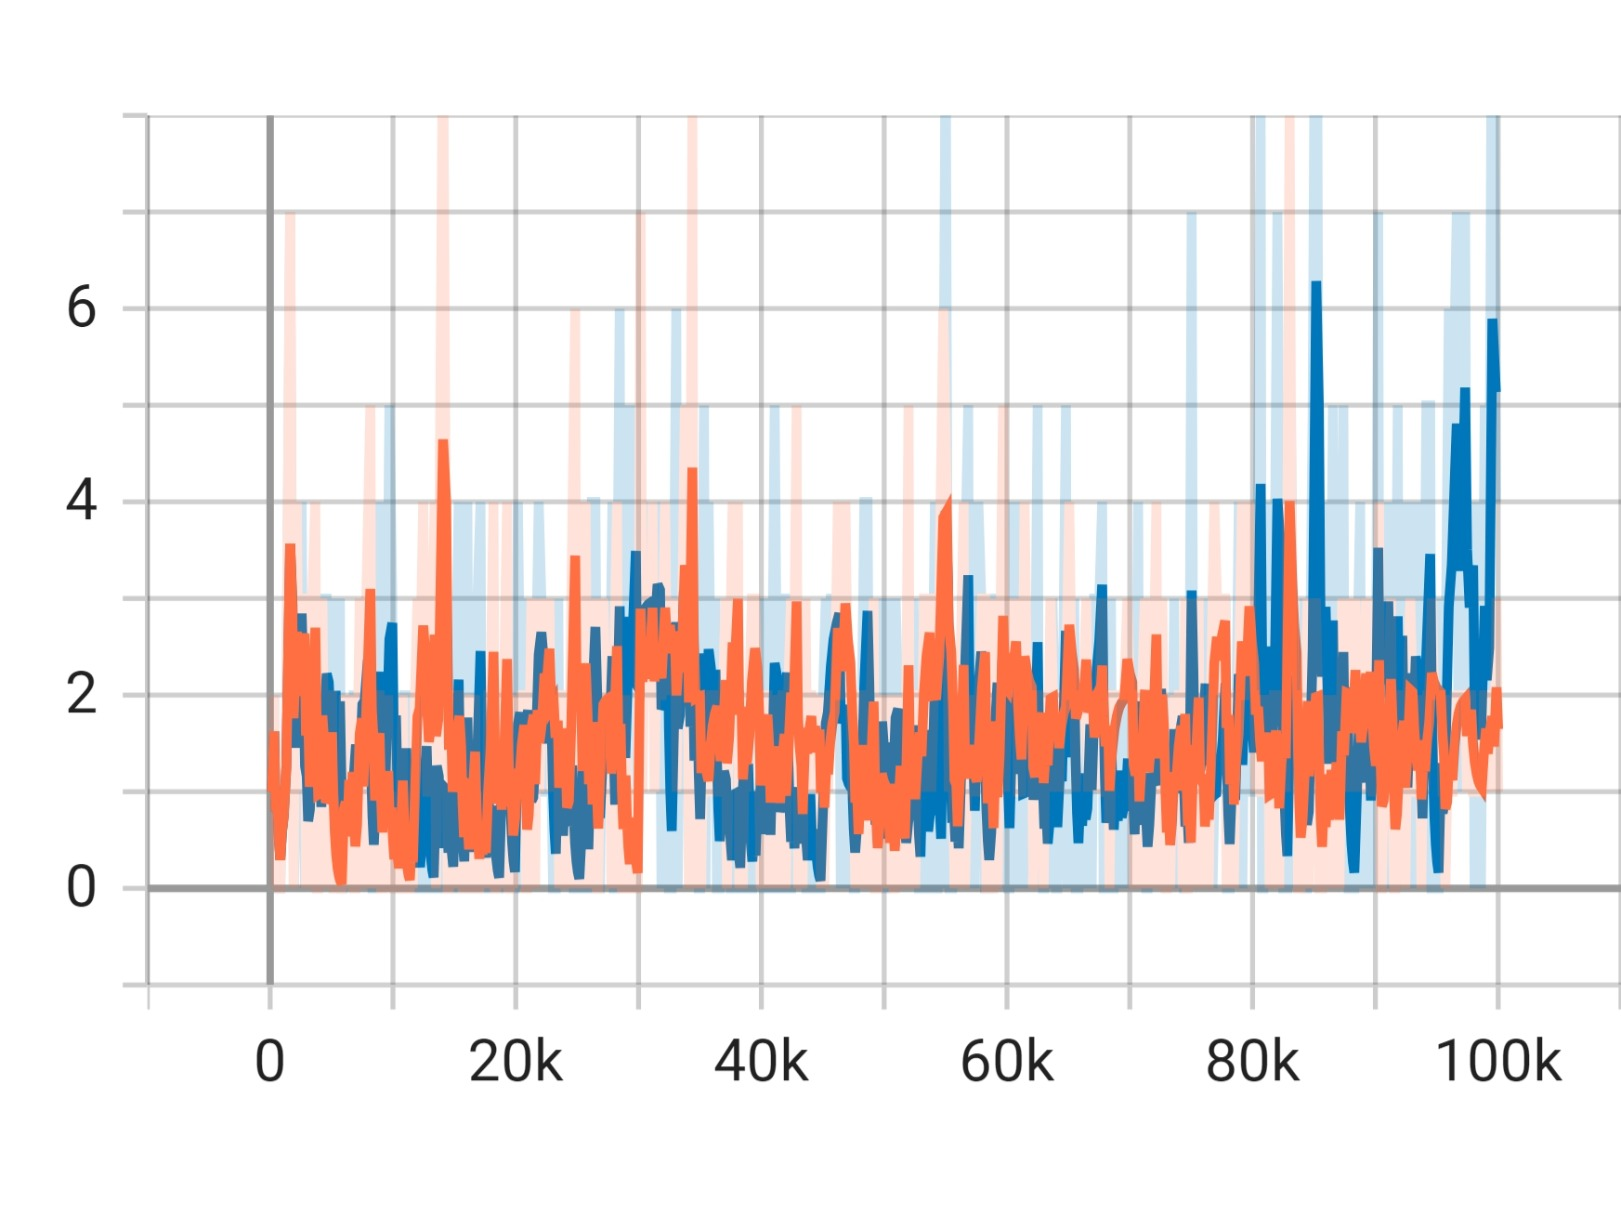
\includegraphics[width=.45\textwidth]{figures/c51/png/charts_episodic_return_1k_10k.jpeg}
		\label{fig:episodic_return_1k_10k}
	}
	\quad
	\subfloat[][\textit{Emissions at 100k steps, \texttt{target\_network\_frequency} = \num{1000} (blue), \num{5000} (red) \num{10000} (orange)}]{
		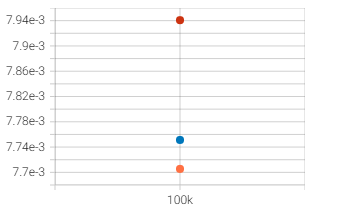
\includegraphics[width=.45\textwidth]{figures/c51/png/emissions_1k_5k_10k.png}
		\label{fig:c51_tuning_emissions}
	}
	\caption{Tuning of \texttt{target\_network\_frequency}.}
	\label{fig:c51_tuning}
\end{figure}

\paragraph{Training Dynamics}

\begin{figure}
	\centering
	\subfloat[][\textit{Episodic length (\texttt{charts\_episodic\_length}). 
	The mean is $\sim$ \num{3500}--\num{4000}, while min--max occasionally spikes above 8000 or even 17500 in some runs.}]{
		\includesvg[width=.45\textwidth]{figures/c51/charts_episodic_length_c51_atari}
		\label{fig:c51_episodic_length}
	}
	\quad
	\subfloat[][\textit{Steps per second (SPS).
	Mean peaks around 160--170, then slowly converges near 140--150.}]{
		\includesvg[width=.45\textwidth]{figures/c51/charts_SPS_c51_atari}
		\label{fig:c51_sps}
	}
	\\[1em]
	\subfloat[][\textit{Overall loss (\texttt{losses/loss}). 
	The mean steadily declines from about 4.0 toward near 2.0 by the end of training.}]{
		\includesvg[width=.45\textwidth]{figures/c51/losses_loss_c51_atari}
		\label{fig:c51_loss}
	}
	\quad
	\subfloat[][\textit{Q-values (\texttt{losses/q\_values}). 
	The mean climbs from near 0 to $\sim$ 4--5, with outliers reaching 6--7.}]{
		\includesvg[width=.45\textwidth]{figures/c51/losses_q_values_c51_atari}
		\label{fig:c51_q_values}
	}
	\caption{C51 training metrics over 100k steps, aggregated (via interpolation) across 32 runs.}
	\label{fig:c51_training_metrics}
\end{figure}

Figure~\vref{fig:c51_training_metrics} shows that certain runs produce extremely long episodes 
(Figure~\ref{fig:c51_episodic_length}), 
while the overall \texttt{SPS} curve (Figure~\ref{fig:c51_sps}) hovers around 140--150 later in training, 
slightly lower than baseline DQN's $\sim$\num{160}. 
The training loss (Figure~\ref{fig:c51_loss}) descends from near 4.0 to 2.0, 
while distributional \texttt{q\_values} (Figure~\ref{fig:c51_q_values}) broaden significantly.

\paragraph{Episodic Return (Aggregated)}

\begin{figure}
	\centering
	\includesvg[width=0.6\textwidth]{figures/c51/charts_episodic_return_human_c51_atari}
	\caption{C51 episodic return (human-normalized), aggregated over 32 runs. 
		Negative scores dominate, especially due to \emph{Boxing}'s steep dips below -10.}
	\label{fig:c51_return_human}
\end{figure}

\begin{figure}
	\centering
	\includesvg[width=0.6\textwidth]{figures/c51/charts_episodic_return_minmax_c51_atari}
	\caption{C51 episodic return (min--max normalized). 
		The mean grows toward 0.25--0.30, indicating moderate performance relative to each game's min--max range.}
	\label{fig:c51_return_minmax}
\end{figure}

Due to extreme negative performance in certain games, such as \emph{Boxing}, 
the human-normalized return (Figure~\vref{fig:c51_return_human}) 
often falls below -1. In min--max (Figure~\vref{fig:c51_return_minmax}), 
the mean approaches $\sim$\num{0.25}--\num{0.30} by 100k steps.

\paragraph{Per-Game Returns}
Figure~\ref{fig:c51_return_pergame_human} presents the human-normalized episodic returns for C51 on a per-game basis. Notably, the game \emph{Boxing} exhibits extremely negative returns—with values plunging below \num{-12}, significantly impacting the overall human-normalized performance. In contrast, games such as \emph{Alien} and \emph{Amidar} show relatively stable and modest returns. Similarly, Figure~\ref{fig:c51_return_pergame_minmax} displays the min--max normalized returns, where \emph{Assault} reaches values above \num{0.5}, while \emph{Pong} remains consistently near zero. These per-game analyses underline the variability of C51's performance across different environments, emphasizing the importance of detailed game-specific evaluations.

\begin{figure}
	\centering
	\includesvg[width=0.6\textwidth]{figures/c51/charts_episodic_return_per_game_human_c51_atari}
	\caption{C51 returns per game (human-normalized). 
		\emph{Boxing} (orange) can plunge below -12, dwarfing improvements in other games.}
	\label{fig:c51_return_pergame_human}
\end{figure}

\begin{figure}
	\centering
	\includesvg[width=0.6\textwidth]{figures/c51/charts_episodic_return_per_game_minmax_c51_atari}
	\caption{C51 returns per game (min--max normalized). 
		\emph{Assault} (green) climbs above 0.5, while \emph{Pong} (cyan) remains near zero.}
	\label{fig:c51_return_pergame_minmax}
\end{figure}

\paragraph{Emissions}
Table~\ref{tab:c51_emissions} details the carbon emissions recorded for C51 across the 32 runs, showing a mean emission of approximately 0.00775\,kg\,CO\textsubscript{2}eq. This value exceeds that of the baseline DQN, which recorded mean emissions of 0.00647\,kg\,CO\textsubscript{2}eq. The additional computational overhead in C51 arises from the need to compute and update a 51-atom probability distribution for the return at each training step, a process that likely increases GPU utilization. Although the absolute emissions remain relatively modest, the consistent increase across runs highlights an important trade-off: while the distributional approach of C51 may offer richer representations of return variability, it does so at the cost of higher energy consumption. This observation is particularly relevant in contexts where energy efficiency and environmental impact are critical considerations.

\begin{table}
	\caption{Carbon emissions (kg\,CO\textsubscript{2}\,eq) for C51 across 32 runs.}
	\label{tab:c51_emissions}
	\centering
	\makebox[\textwidth]{%
	\begin{tabular}{lcccccccc}
		\toprule
		\textbf{Algorithm} & \textbf{mean} & \textbf{std} & \textbf{median} & 
		\textbf{q25} & \textbf{q75} & \textbf{min} & \textbf{max} & \textbf{iqmean} \\
		\midrule
		C51 & 0.007750 & 0.0003042 & 0.007655 & 0.007489 & 0.008099 & 0.007410 & 0.008257 & 0.007679 \\
		\bottomrule
	\end{tabular}
	}
\end{table}

\begin{figure}
	\centering
	\includesvg[width=0.55\textwidth]{figures/c51/emissions_dqn_c51}
	\caption{Mean emissions: C51 (magenta) at $\sim$\num{0.00775}\,kg vs.\ DQN (gold) at $\sim$\num{0.00647}\,kg.}
	\label{fig:c51_vs_dqn_emissions}
\end{figure}

\paragraph{Evaluation Results}
The overall final evaluation of C51, conducted over 10 episodes per run and aggregated across 32 runs, is summarized in Table~\ref{tab:c51_eval_overall}. On the human-normalized scale, C51 achieves a mean return of \num{-1.0811} with a high standard deviation of \num{3.2862} and a range from \num{-12.8810} to \num{0.7770}, reflecting significant variability driven by outlier performances (notably in \emph{Boxing}). In contrast, min--max normalization yields a mean of 0.2503 with a smaller standard deviation of \num{0.2568} and a range from \num{0.0} to \num{0.8270}, indicating a more balanced distribution of performance scores. Furthermore, Table~\ref{tab:c51_eval_gamewise} provides a per-game breakdown, where for example \emph{Boxing} registers a human-normalized mean of \num{-9.3869}, while other games such as \emph{Alien} and \emph{Amidar} exhibit near-neutral scores. These results offer a nuanced perspective on C51's performance across different games and normalization methods.

\begin{table}
	\caption{Overall final evaluation (10 episodes each) for C51 across 32 runs.}
	\label{tab:c51_eval_overall}
	\centering
	\makebox[\textwidth]{%
	\begin{tabular}{lcccccccc}
		\toprule
		\textbf{Normalization} & \textbf{mean} & \textbf{std} & \textbf{median} & 
		\textbf{q25} & \textbf{q75} & \textbf{min} & \textbf{max} & \textbf{iqmean} \\
		\midrule
		\textbf{Human}   & -1.0811 & 3.2862 & 0.0 & -0.0132 & 0.0418 & -12.8810 & 0.7770 & 0.00684 \\
		\textbf{Min--Max}& 0.2503 & 0.2568 & 0.2005 & 0.0 & 0.4419 & 0.0 & 0.8270 & 0.13997 \\
		\bottomrule
	\end{tabular}
	}
\end{table}

\begin{table}
	\caption{Per-game final evaluation for C51 (human- vs.\ min--max normalized). 
		Each row aggregates 40 total episodes (10 per seed).}
	\label{tab:c51_eval_gamewise}
	\centering
	\begin{tabular}{llcccc}
		\toprule
		\textbf{Game} & \textbf{Norm} & \textbf{mean} & \textbf{std} & \textbf{min} & \textbf{max}\\
		\midrule
		Alien & Human    & -0.0149 & 0.0127 & -0.0343 & 0.00635 \\
		& Min--Max & 0.0321  & 0.0211 & 0.0     & 0.0675 \\
		\cmidrule{1-6}
		Amidar & Human   & 0.0336  & 0.0153 & 0.00431 & 0.0678 \\
		& Min--Max & 0.2851 & 0.1181 & 0.0599  & 0.5484 \\
		\cmidrule{1-6}
		Assault & Human  & 0.1994  & 0.1467 & -0.0262 & 0.3860 \\
		& Min--Max & 0.5434 & 0.2229 & 0.2005  & 0.8270 \\
		\cmidrule{1-6}
		Boxing & Human   & -9.3869 & 2.6728 & -12.8810 & -4.7857 \\
		& Min--Max & 0.4548  & 0.0870 & 0.3411   & 0.6047 \\
		\cmidrule{1-6}
		Breakout & Human & 0.1478  & 0.2072 & -0.0565 & 0.4751 \\
		& Min--Max & 0.1618 & 0.1641 & 0.0     & 0.4211 \\
		\cmidrule{1-6}
		Freeway & Human  & 0.3632  & 0.3688 & 0.0      & 0.7770 \\
		& Min--Max & 0.3839 & 0.3899 & 0.0     & 0.8214 \\
		\cmidrule{1-6}
		MsPacman & Human & 0.0189  & 0.0176 & -0.0057 & 0.0483 \\
		& Min--Max & 0.1410 & 0.0707 & 0.0419 & 0.2592 \\
		\cmidrule{1-6}
		Pong & Human     & -0.01   & $5.27\times 10^{-18}$ & -0.01 & -0.01 \\
		& Min--Max & 0.0     & 0.0     & 0.0     & 0.0 \\
		\bottomrule
	\end{tabular}
\end{table}

\paragraph{Comparison with Baseline DQN}
Overall, C51's human-normalized final mean is \num{-1.0811}, pulled down by severe negative performance in \emph{Boxing} (around $-9.39$). Even ignoring that outlier, other titles do not significantly outperform baseline DQN's \num{0.1353}. In min--max scale, C51's \num{0.2503} is also lower than DQN's \num{0.3802}. Emissions, by contrast, are higher ($\sim$\num{0.00775}\,kg vs.\ DQN's \num{0,00647}), reflecting the overhead of computing a 51-atom return distribution each update.

\paragraph{Observations}
\begin{itemize}
	\item \textbf{Distributional Advantage:} 
	Although distributional RL can better capture risk or reward variance, 
	100k steps may be insufficient to realize its full potential.
	\item \textbf{Performance:} 
	Human-norm is \num{-1.0811} vs.\ DQN's \num{0.1353}, with many games remaining near/below zero. 
	Min--max is \num{0.2503} vs.\ \num{0.3802}.
	\item \textbf{Emissions:}
	C51 uses $\sim$\num{0.00775}\,kg\,CO\textsubscript{2}\,eq, higher than DQN's \num{0.00647}, 
	likely due to distributional overhead.
	\item \textbf{Target Network Frequency:}
	Testing 1k, 5k, and 10k found 1k gave decent stability and moderate power usage.
\end{itemize}

In summary, C51 did not outperform the baseline DQN in this 100k-step Atari benchmark, 
though distributional RL may yield advantages over longer runs or with additional tuning.


\subsection{Overall Comparison of DQN-Based Algorithms}
\label{subsec:dqn_overall_comparison}

In this section, we synthesize the results of all five DQN-based algorithms:
\begin{itemize}
	\item \textbf{Baseline DQN} (no additional tweaks)
	\item \textbf{Double DQN} (mitigating Q-value overestimation)
	\item \textbf{Prioritized Experience Replay (PER)} (sampling transitions by TD-error priority)
	\item \textbf{Dueling DQN} (separating state-value from advantage)
	\item \textbf{C51} (distributional RL with a categorical action distribution)
\end{itemize}
We compare them on two axes: final performance (evaluated in both human- and min--max-normalized scales) and carbon emissions. 

\paragraph{Aggregated Final Returns and Emissions}
Table~\ref{tab:dqn_overall} compiles the final evaluation means from Sections \ref{subsubsec:dqn_baseline}, \ref{subsubsec:double_dqn}, \ref{subsubsec:per}, \ref{subsubsec:dueling_dqn}, and \ref{subsubsec:c51}. We list each method's mean episodic return under both normalization schemes, along with its mean carbon footprint. For completeness, we include standard deviations (\texttt{std}) and other statistics. Table~\ref{tab:dqn_overall_iqm} extends the previous summary table by including the interquartile mean (IQM)~\cite{agarwal:statistical_precipice} for each of the three metrics. Recall that IQM is a robust estimator of central tendency, averaging only the middle 50\% of data points (between the 25th and 75th percentiles), thus mitigating the impact of extreme outliers. Follows a brief discussion of the performance of every algorithm.

\begin{table}
	\caption{Overall final evaluation and emissions for DQN-based algorithms. 
		Human-/min--max-normalized performance are the global means across 32 runs (8 games, 4 seeds). 
		Emissions are reported in kg\,CO\textsubscript{2}\,eq. 
		Lower or negative human-norm means indicate below-human performance on average (e.g.\ in \emph{Boxing}), 
		whereas higher min--max means imply better relative scores.}
	\label{tab:dqn_overall}
	\centering
	\begin{tabular}{lccccc}
		\toprule
		& \multicolumn{2}{c}{\textbf{Final Episodic Return (Mean)}} & 
		\multicolumn{1}{c}{\textbf{Emissions}} \\
		\cmidrule(lr){2-3} \cmidrule(lr){4-4}
		\textbf{Algorithm} & \textbf{Human Norm} & \textbf{Min--Max} & \textbf{(kg\,CO\textsubscript{2}\,eq)} \\
		\midrule
		\textbf{DQN (baseline)} & 0.1353 & 0.3802 & 0.00647 \\
		\textbf{Double DQN}     & 0.0226 & 0.3737 & 0.00667 \\
		\textbf{PER}            & 0.0607 & 0.3533 & 0.00725 \\
		\textbf{Dueling DQN}    & 0.1860 & 0.3849 & 0.00689 \\
		\textbf{C51}            & -1.0811 & 0.2503 & 0.00775 \\
		\bottomrule
	\end{tabular}
\end{table}

\begin{table}
	\caption{DQN‐Based Algorithms: Final Returns (Human \& Min--Max Norm) \emph{vs.} Emissions,
		including both Mean and Interquartile Mean (IQM). 
		Data are aggregated over 32 runs (8 Atari games $\times$ 4 seeds). 
		Negative human‐norm means can stem from poor performance in certain games 
		(e.g.\ \emph{Boxing} with highly negative scores).}
	\label{tab:dqn_overall_iqm}
	\centering
	\makebox[\textwidth]{%
		\begin{tabular}{lrrrrrr}
			\toprule
			& \multicolumn{2}{c}{\textbf{Human‐Norm Return}} 
			& \multicolumn{2}{c}{\textbf{Min--Max Return}}
			& \multicolumn{2}{c}{\textbf{Emissions (kg\,CO\textsubscript{2})}} \\
			\cmidrule(lr){2-3}\cmidrule(lr){4-5}\cmidrule(lr){6-7}
			\textbf{Algorithm}
			& \textbf{Mean} & \textbf{IQM}
			& \textbf{Mean} & \textbf{IQM}
			& \textbf{Mean} & \textbf{IQM} \\
			\midrule
			\textbf{DQN} 
			& 0.1353 & 0.1137 
			& 0.3802 & 0.3426 
			& 0.00647 & 0.00637 \\
			\textbf{Double DQN} 
			& 0.0226 & 0.0894 
			& 0.3737 & 0.3272 
			& 0.00667 & 0.00656 \\
			\textbf{PER} 
			& 0.0607 & 0.0813 
			& 0.3533 & 0.3087 
			& 0.00725 & 0.00716 \\
			\textbf{Dueling DQN} 
			& 0.1860 & 0.1020 
			& 0.3849 & 0.3454 
			& 0.00689 & 0.00678 \\
			\textbf{C51} 
			& $-1.0811$ & 0.00684 
			& 0.2503 & 0.1400 
			& 0.00775 & 0.00768 \\
			\bottomrule
		\end{tabular}
	}
\end{table}

\begin{description}
	\item[Dueling DQN] achieves the highest human-norm mean (\num{0.1860}), though min--max is only slightly above baseline DQN (\num{0.3849} vs.\ \num{0.3802}). Its moderate overhead in computations yields emissions of \num{0.00689}\,kg, just above baseline.
	\item[Double DQN] has a low human-norm mean (\num{0.0226}) but a reasonably strong min--max mean (\num{0.3737}). Some games suffer from negative outliers (e.g.\ \emph{Boxing}), but overall it matches baseline DQN in relative scale.
	\item[PER] does not strongly outperform DQN in short (100k-step) training, scoring \num{0.0607} human-norm and \num{0.3533} min--max, with slightly higher emissions (\num{0.00725}\,kg). Prioritizing TD errors may show more benefit in longer runs.
	\item[C51] exhibits the largest negative dip on human-norm (\num{-1.0811}), largely due to extreme results in \emph{Boxing} and a few other titles, but obtains \num{0.2503} in min--max. It also has the largest emissions (\num{0.00775}\,kg) among these five, reflecting the overhead of a distributional approach with 51 “atoms”.
	\item[Baseline DQN] remains a strong reference point. Though not best in any single metric, it has decent performance across games (especially \num{0.3802} in min--max), while keeping the lowest carbon footprint (\num{0.00647}\,kg).
\end{description}

\paragraph{Noteworthy points:}
\begin{itemize}
	\item \emph{Human‐Norm vs.\ IQM.} 
	Some methods (\emph{e.g.}, Double DQN, C51) 
	exhibit a large discrepancy between the mean and IQM in human‐normalized returns, 
	indicating a handful of extreme outliers (often due to specific games like Boxing).
	\item \emph{Dueling DQN.} 
	Its mean is highest in human‐norm (\num{0.1860}), 
	but the IQM (\num{0.1020}) is closer to baseline DQN's \num{0.1137}, 
	suggesting moderate overall gains once outliers are downweighted.
	\item \emph{C51's Negative Mean.} 
	With \num{-1.08} in human‐norm, C51 suffers from severely negative outliers; 
	however, its IQM (\num{0.00684}) sits just above zero, reflecting that only a few seeds/games 
	are catastrophic outside Boxing.
	\item \emph{Emissions Overhead.} 
	Distributional (C51) and prioritized (PER) methods do have higher carbon costs 
	(around \num{0.0077}\,kg and \num{0.00725}\,kg, respectively) than vanilla DQN (\num{0.00647}\,kg). 
	The IQM for emissions shows a similar trend (\num{0.00768} and \num{0.00716} vs.\ \num{0.00637}).
\end{itemize}

Altogether, adding the IQM metric helps to highlight the presence of large outliers
in short 100k‐step runs. Dueling emerges as a modest improvement on baseline DQN
once extreme seeds are downweighted, whereas C51 and PER do not yet exhibit 
strong benefits for the added cost in short training scenarios.

%%%%%%%%%%%%%%%%%%%%%%%%%%%%%

\paragraph{Scatter Plots of Emissions vs.\ Performance}
To visually depict the trade-off between carbon footprint and final performance,
Figures~\ref{fig:dqn_scatter_mean_iqm} and~\ref{fig:dqn_scatter_mean_mean} 
show scatter plots of \texttt{Mean~Emissions} on the x-axis against 
(\emph{i}) the \texttt{IQMean} or 
(\emph{ii}) the \texttt{Mean} of final evaluation on the y-axis. 
We plot both the human-normalized and min--max normalized variants.

\begin{figure}
	\centering
	\subfloat[][\textit{Human Norm: Mean Emissions vs.\ IQMean Evaluation}]{
		\includesvg[width=.45\textwidth]{figures/dqn_based_comparison/scatter_iqmean_human_dqn_based_comparison}
		\label{fig:dqn_scatter_iqm_human}
	}
	\quad
	\subfloat[][\textit{Min--Max: Mean Emissions vs.\ IQMean Evaluation}]{
		\includesvg[width=.45\textwidth]{figures/dqn_based_comparison/scatter_iqmean_minmax_dqn_based_comparison}
		\label{fig:dqn_scatter_iqm_minmax}
	}
	\caption{Scatter: Mean Emissions vs.\ Interquartile Mean (IQM) final evaluation, for DQN-based algorithms. 
		C51 (magenta) appears far to the right (highest emissions) 
		and near the bottom in human norm, though it's closer in min--max. 
		DQN and Double DQN cluster with relatively low emissions.}
	\label{fig:dqn_scatter_mean_iqm}
\end{figure}

\begin{figure}
	\centering
	\subfloat[][\textit{Human Norm: Mean Emissions vs.\ Mean Evaluation}]{
		\includesvg[width=.45\textwidth]{figures/dqn_based_comparison/scatter_mean_human_dqn_based_comparison}
		\label{fig:dqn_scatter_mean_human}
	}
	\quad
	\subfloat[][\textit{Min--Max: Mean Emissions vs.\ Mean Evaluation}]{
		\includesvg[width=.45\textwidth]{figures/dqn_based_comparison/scatter_mean_minmax_dqn_based_comparison}
		\label{fig:dqn_scatter_mean_minmax}
	}
	\caption{Scatter: Mean Emissions vs.\ Mean final evaluation, for DQN-based algorithms. 
		Again, C51 (magenta) is an outlier with higher emissions and negative (human) or low (min--max) returns. 
		Dueling (blue) has moderate emissions and the highest human-norm performance.}
	\label{fig:dqn_scatter_mean_mean}
\end{figure}

\paragraph{Game-by-Game Observations}
When looking individually per environment:
\begin{itemize}
	\item \emph{Boxing} (Figure~\ref{fig:boxing_comparison}) heavily skews human-normalized averages for PER and especially C51, 
	yielding strongly negative means. 
	Dueling or Double DQN often handle Boxing more stably.
	\item \emph{Freeway} (Figure~\ref{fig:freeway_comparison}) is comparatively easier, so all variants converge to near-human or above. 
	PER and Dueling both score well here. 
	\item \emph{Assault} (Figure~\vref{fig:assault_comparison}) sees moderate or high min--max normalized returns across the board; 
	distributional methods like C51 can do fairly well in some seeds, but not enough to beat DQN or Dueling on average.
\end{itemize}

%----------------------
% 1) BOXING
%----------------------
\begin{figure}
	\centering
	\subfloat[][\textit{Human Norm: Boxing}]{
		\includesvg[width=.45\textwidth]{figures/dqn_based_comparison/charts_episodic_return_human_comparison_BoxingNoFrameskip-v4_dqn}
		\label{fig:boxing_human_dqn}
	}
	\quad
	\subfloat[][\textit{Min--Max: Boxing}]{
		\includesvg[width=.45\textwidth]{figures/dqn_based_comparison/charts_episodic_return_minmax_comparison_BoxingNoFrameskip-v4_dqn}
		\label{fig:boxing_minmax_dqn}
	}
	\caption{Comparison of DQN-based algorithms on \text{Boxing}. 
		The human-normalized scale (\textit{left}) highlights large negative dips, especially for C51 and PER. 
		Min--max normalized (\textit{right}) shows moderate ranges for most algorithms.}
	\label{fig:boxing_comparison}
\end{figure}

%----------------------
% 2) FREEWAY
%----------------------
\begin{figure}
	\centering
	\subfloat[][\textit{Human Norm: Freeway}]{
		\includesvg[width=.45\textwidth]{figures/dqn_based_comparison/charts_episodic_return_human_comparison_FreewayNoFrameskip-v4_dqn}
		\label{fig:freeway_human_dqn}
	}
	\quad
	\subfloat[][\textit{Min--Max: Freeway}]{
		\includesvg[width=.45\textwidth]{figures/dqn_based_comparison/charts_episodic_return_minmax_comparison_FreewayNoFrameskip-v4_dqn}
		\label{fig:freeway_minmax_dqn}
	}
	\caption{Comparison of DQN-based algorithms on \textit{Freeway}. 
		All methods converge relatively quickly to near-human or above. 
		PER and Dueling typically perform strongly on this environment.}
	\label{fig:freeway_comparison}
\end{figure}

%----------------------
% 3) ASSAULT
%----------------------
\begin{figure}
	\centering
	\subfloat[][\textit{Human Norm: Assault}]{
		\includesvg[width=.45\textwidth]{figures/dqn_based_comparison/charts_episodic_return_human_comparison_AssaultNoFrameskip-v4_dqn}
		\label{fig:assault_human_dqn}
	}
	\quad
	\subfloat[][\textit{Min--Max: Assault}]{
		\includesvg[width=.45\textwidth]{figures/dqn_based_comparison/charts_episodic_return_minmax_comparison_AssaultNoFrameskip-v4_dqn}
		\label{fig:assault_minmax_dqn}
	}
	\caption{Comparison of DQN-based algorithms on \textit{Assault}, 
		showing human-normalized (\textit{left}) and min--max normalized (\textit{right}) 
		final returns over 100k steps. 
		Distributional methods (C51) can excel in some seeds but not enough to surpass Dueling/DQN on average.}
	\label{fig:assault_comparison}
\end{figure}

\paragraph{Emissions and Efficiency}
As indicated by both Table~\ref{tab:dqn_overall}, Table~\ref{tab:dqn_overall_iqm}, 
and the scatter plots (Figures~\ref{fig:dqn_scatter_mean_iqm}--\ref{fig:dqn_scatter_mean_mean}), 
C51 has the highest mean emissions ($\sim$\num{0.00775}\,kg, 
while PER also exceeds baseline levels at \num{0.00725}\,kg. 
DQN remains the lowest (\num{0.00647}\,kg). 
In short 100k-step training, the benefits of distributional or prioritized approaches 
do not fully emerge, whereas their computational overhead (and hence emissions) is quite tangible.

\paragraph{Emissions Barplot}

Figure~\ref{fig:dqn_comp_emissions_bar} illustrates a direct barplot comparison
of the average emissions (with error bars for standard deviation) for the five methods.
\begin{figure}
	\centering
	\includesvg[width=0.48\textwidth]{figures/dqn_based_comparison/barplot_emissions_dqn_based_comparison}
	\caption{Emissions Barplot (DQN-based Comparison). 
		C51 (magenta) leads with $\sim$\num{0.0078}\,kg, while DQN (gold) is at the low end (\num{0.00647}).}
	\label{fig:dqn_comp_emissions_bar}
\end{figure}

\paragraph{Steps Per Second (SPS) Comparison}
Figure~\ref{fig:dqn_comp_sps} displays the aggregated SPS for each of the five DQN-based algorithms.
DQN (gold) and Double DQN (red) generally achieve the highest throughput, stabilizing around
160--170 steps per second. PER (green) and Dueling (blue) see moderate slowdowns, often converging
in the 140--160 range. C51 (magenta), with its added distributional overhead, tends to maintain
the lowest SPS, sometimes falling below 140. These throughput differences align with the 
emissions data (Tables~\ref{tab:dqn_overall} and~\vref{tab:dqn_overall_iqm}), reinforcing that more
computationally demanding methods can incur higher carbon footprints, even within a 
relatively short 100k-step training horizon.

\begin{figure}
	\centering
	\includesvg[width=0.65\textwidth]{figures/dqn_based_comparison/sps_dqn_based}
	\caption{Comparison of Steps Per Second (SPS) over 100k steps for the five DQN-based algorithms. 
		Baseline DQN and Double DQN generally run fastest, while C51 exhibits the slowest throughput.}
	\label{fig:dqn_comp_sps}
\end{figure}

\paragraph{Key Takeaways}
\begin{itemize}
	\item \emph{Dueling DQN} shows the best human-norm mean (\num{0.1860}), 
	or second-best min--max (\num{0.3849}). Its overhead is modest.
	\item \emph{Double DQN} is cheap in energy and helps curb Q-value inflation, 
	but does not necessarily raise final returns in short runs (\num{0.0226} human, \num{0.3737} min--max).
	\item \emph{PER} is also more costly (\num{0.00725}\,kg) with only slight gains in 100k steps, 
	suggesting PER's advantage might need longer training to appear.
	\item \emph{C51} is the outlier in both emissions and negative returns (human), 
	though its IQM is far less extreme, indicating that only a few seeds/games are catastrophic.
	\item \emph{Baseline DQN} remains a viable option at 100k steps, 
	balancing decent performance and the lowest emissions of the five variants.
\end{itemize}

\subsection{Policy Gradient Algorithms}
This section presents results for the three policy gradient methods.

\subsubsection{REINFORCE}
\label{subsubsec:reinforce}
REINFORCE is a classical policy gradient algorithm, discussed in Chapter 13 of~\cite{sutton:rl}. In its pure form, the algorithm updates the policy parameters using the full return observed in an episode, without any baseline or actor–critic modifications, thus adhering closely to the theoretical formulation. Although it enjoys strong theoretical convergence guarantees in the limit of infinite interactions, in practice (especially over a short 100k-step training horizon) REINFORCE exhibits high variance, leading to unstable learning. Nonetheless, in our implementation we follow the standard formulation as closely as possible, with only minor modifications such as a slight learning rate annealing. 

\paragraph{(Hyper)Parameters}
We adopt a standard configuration for REINFORCE similar to prior work on policy gradient methods. Table~\ref{tab:reinforce_hyperparams} summarizes the key hyperparameters used in our experiments. In our setup, only the environment identifier (\texttt{env\_id}) and the random seed (\texttt{seed}) vary across runs. Notably, the learning rate is set to \num{0.00025} and the discount factor (\(\gamma\)) to \num{0.99}.

\begin{table}
	\caption{Key hyperparameters for the REINFORCE algorithm. Only \texttt{env\_id} and \texttt{seed} vary across runs.}
	\label{tab:reinforce_hyperparams}
	\centering
	\begin{tabular}{ll}
		\toprule
		\textbf{Parameter} & \textbf{Value} \\
		\midrule
		\texttt{exp\_name}            & reinforce\_atari \\
		\texttt{seed}                 & 1..4 \\
		\texttt{torch\_deterministic} & True \\
		\texttt{cuda}                 & True \\
		\texttt{track}                & True \\
		\texttt{wandb\_project\_name} & rlsb \\
		\texttt{capture\_video}       & False \\
		\texttt{save\_model}          & True \\
		\texttt{env\_id}              & e.g.\ AmidarNoFrameskip-v4 \\
		\texttt{total\_timesteps}     & 100000 \\
		\texttt{learning\_rate}       & 0.00025 \\
		\texttt{num\_envs}            & 1 \\
		\texttt{gamma}                & 0.99 \\
		\bottomrule
	\end{tabular}
\end{table}

\paragraph{Hyperparameter Tuning}
We tested two primary learning rates ($1\times10^{-4}$ vs.\ $2.5\times10^{-4}$), each with a slight annealing schedule over the 100k steps. 
Ultimately, $2.5\times10^{-4}$ converged more reliably in short‐run experiments, as illustrated in Figure~\ref{fig:reinforce_lr_tuning}. 
However, even the better (and higher) learning rate sees limited improvements in just 100k steps, reflecting REINFORCE's inherent high variance.
In our experiments, we also tested the impact of (removing) reward clipping; however, probably because we already normalize returns as a best practice to stabilize learning, its presence or absence had no measurable effect, so we kept it for consistency with the other methods tested.
\begin{figure}
	\centering
	\subfloat[][\textit{Episodic Return (Raw) for Two LRs}]{
		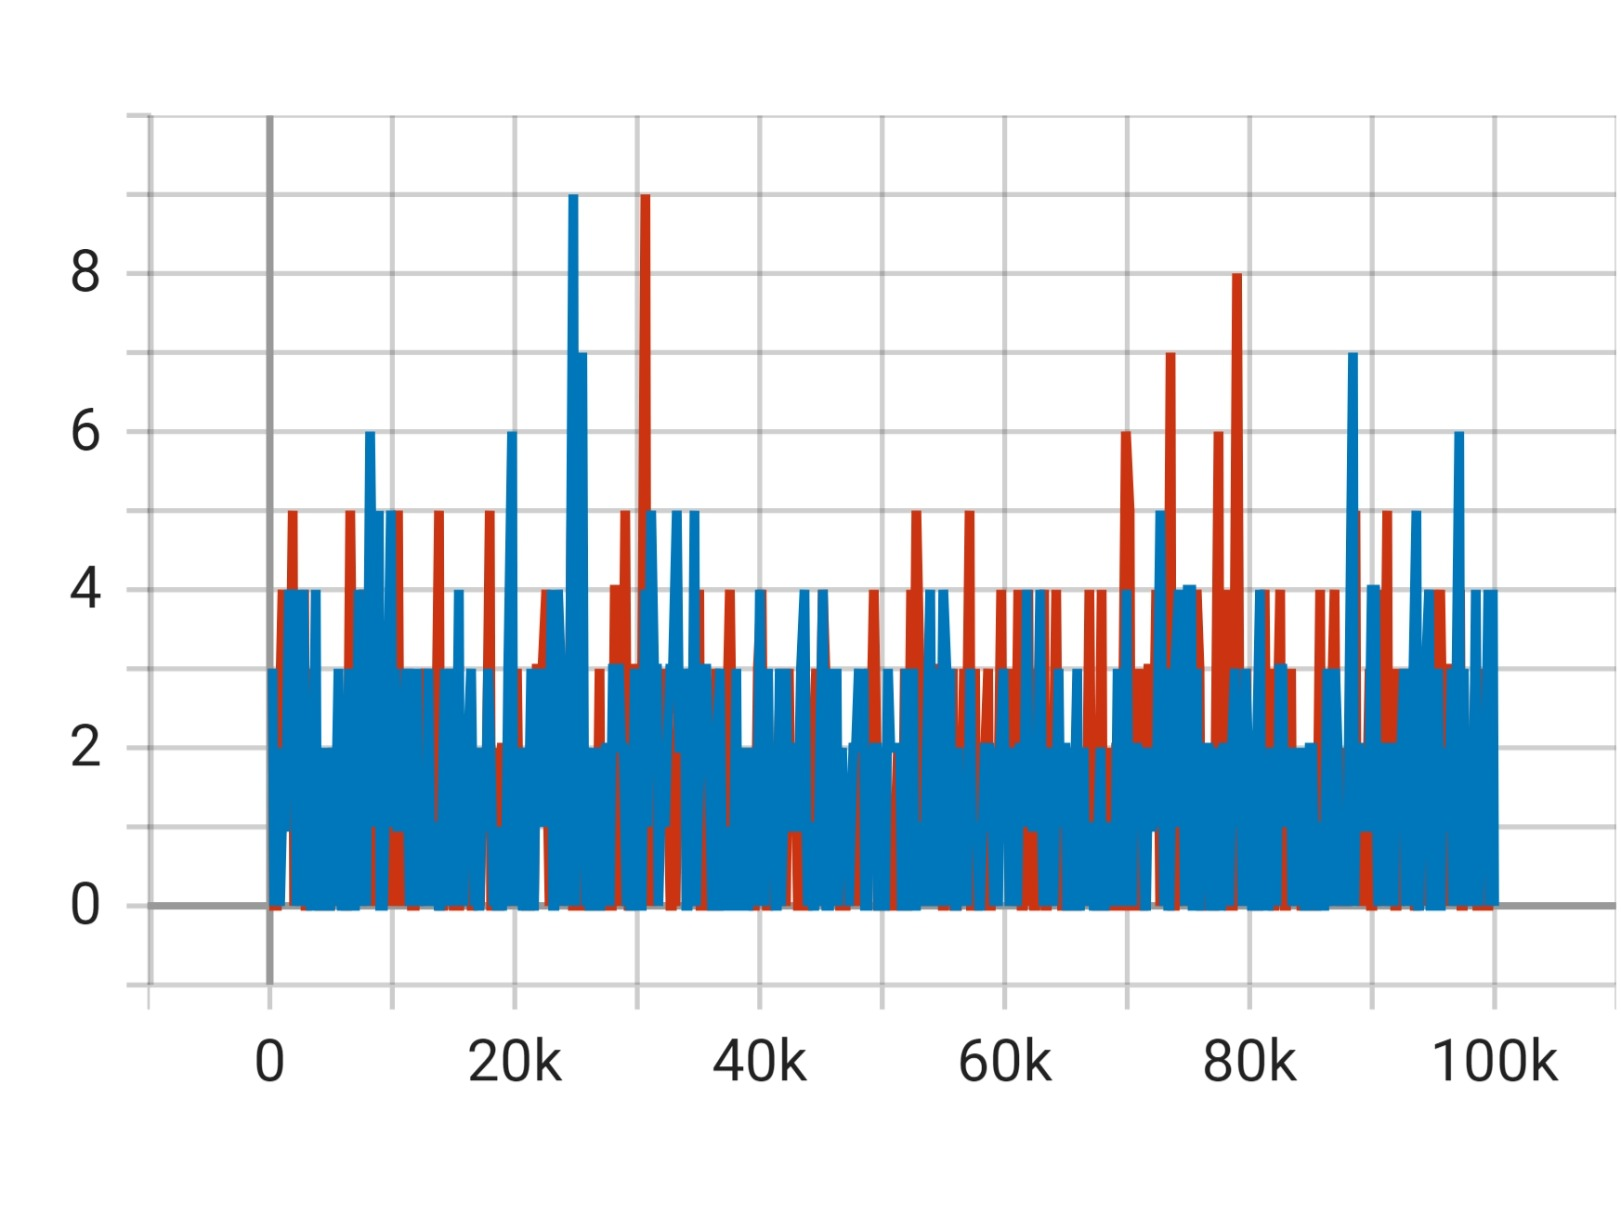
\includegraphics[width=.45\textwidth]{figures/reinforce/png/reinforce_lr_tuning_episodic_return.jpeg}
		\label{fig:reinforce_lr_tuning_return}
	}
	\quad
	\subfloat[][\textit{Learning Rate Schedules}]{
		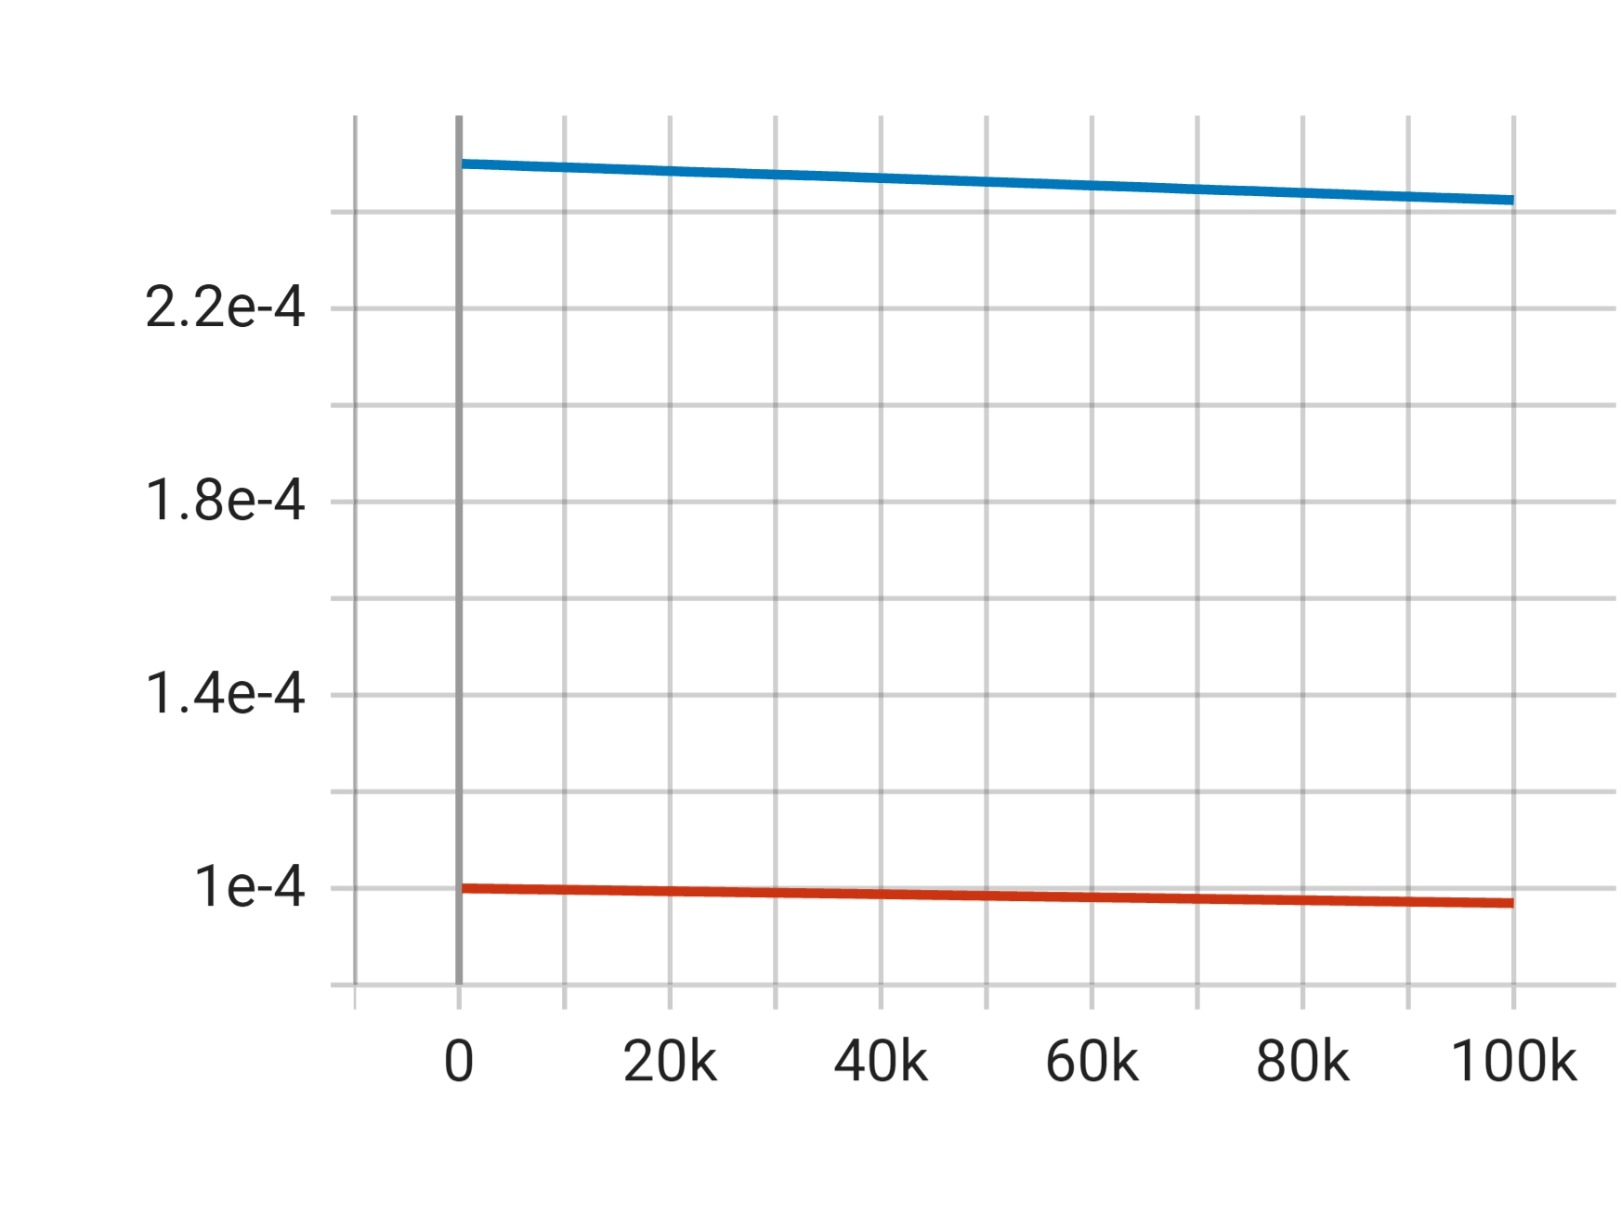
\includegraphics[width=.45\textwidth]{figures/reinforce/png/reinforce_lr_tuning_learning_rate.jpeg}
		\label{fig:reinforce_lr_tuning_lr}
	}
	\caption{\emph{REINFORCE Learning Rate Tuning.} Two learning rates ($1\times10^{-4}$ in red, $2.5\times10^{-4}$ in blue) 
		both with minimal decay. The higher LR eventually performed better, although volatility remained high.}
	\label{fig:reinforce_lr_tuning}
\end{figure}

\paragraph{Aggregated Returns}
Figures~\ref{fig:reinforce_return_human_agg} and~\ref{fig:reinforce_return_minmax_agg} show the aggregated episodic returns (mean $\pm$ min–max envelope) 
for human‐normalized and min--max normalized scales:
\begin{itemize}
	\item \emph{Human norm} typically hovers around zero—some seeds spike up to +4 or +5, others dip to -2 or -3.
	\item \emph{Min--max norm} plateaus around 0.15--0.20, but occasionally climbs near 0.8 in certain runs.
\end{itemize}

\begin{figure}
	\centering
	\subfloat[][\textit{Human‐Normalized Returns (Aggregated)}]{
		\includesvg[width=.45\textwidth]{figures/reinforce/charts_episodic_return_human_reinforce_atari}
		\label{fig:reinforce_return_human_agg}
	}
	\quad
	\subfloat[][\textit{Min--Max Returns (Aggregated)}]{
		\includesvg[width=.45\textwidth]{figures/reinforce/charts_episodic_return_minmax_reinforce_atari}
		\label{fig:reinforce_return_minmax_agg}
	}
	\caption{\textit{REINFORCE Aggregated Episodic Returns.} 
		Strong variance across seeds/games yields a wide min-max band in both normalizations. 
		Mean in human norm often oscillates near zero, while min-max hovers around 0.15-0.20.}
	\label{fig:reinforce_returns_agg}
\end{figure}

\paragraph{Per‐Game Breakdown}
Figure~\ref{fig:reinforce_pergame_return} displays the same returns (human \& min--max) 
but \emph{separated by environment}:
\begin{itemize}
	\item \emph{Boxing} shows extreme positive and negative values in human‐norm.
	\item \emph{Freeway} remains nearly flat (close to zero).
	\item \emph{Assault} in min--max normalization reaches approximately 0.4 in some seeds, outpacing many other tasks.
\end{itemize}

\begin{figure}
	\centering
	\subfloat[][\textit{Per‐Game: Human Norm}]{
		\includesvg[width=.45\textwidth]{figures/reinforce/charts_episodic_return_per_game_human_reinforce_atari}
		\label{fig:reinforce_return_pergame_human}
	}
	\quad
	\subfloat[][\textit{Per‐Game: Min--Max Norm}]{
		\includesvg[width=.45\textwidth]{figures/reinforce/charts_episodic_return_per_game_minmax_reinforce_atari}
		\label{fig:reinforce_return_pergame_minmax}
	}
	\caption{\textit{REINFORCE Returns by Environment.} 
	Variability is evident across different Atari games, with Boxing and Assault exhibiting the highest fluctuations.}
	\label{fig:reinforce_pergame_return}
\end{figure}

\paragraph{Training Metrics}
Additional training metrics are shown in Figures~\ref{fig:reinforce_trainmetrics1} and~\ref{fig:reinforce_trainmetrics2}. The episode length stabilizes near \num{3800}–\num{4000} steps (Figure~\ref{fig:reinforce_epilen}), while the steps per second (SPS) plateaus between 150 and 170 (Figure~\ref{fig:reinforce_sps}). The policy loss (raw) fluctuates significantly due to high-variance returns, and the learning rate drifts minimally from $2.5\times10^{-4}$ to approximately $2.4\times10^{-4}$ over 100k steps.
\begin{figure}
	\centering
	\subfloat[][\textit{Episode Length}]{
		\includesvg[width=.45\textwidth]{figures/reinforce/charts_episodic_length_reinforce_atari}
		\label{fig:reinforce_epilen}
	}
	\quad
	\subfloat[][\textit{Steps Per Second (SPS)}]{
		\includesvg[width=.45\textwidth]{figures/reinforce/charts_SPS_reinforce_atari}
		\label{fig:reinforce_sps}
	}
	\caption{\textit{REINFORCE Episode Length and Throughput.} 
		The average length stabilizes near 3800–4000 steps; 
		min–max can exceed 7000–8000 in some seeds. 
		SPS plateaus around 150–170.}
	\label{fig:reinforce_trainmetrics1}
\end{figure}

\begin{figure}
	\centering
	\subfloat[][\textit{Policy Loss (raw)}]{
		\includesvg[width=.45\textwidth]{figures/reinforce/losses_loss_reinforce_atari}
		\label{fig:reinforce_loss}
	}
	\quad
	\subfloat[][\textit{Learning Rate (Minimal Decay)}]{
		\includesvg[width=.45\textwidth]{figures/reinforce/charts_learning_rate_reinforce_atari}
		\label{fig:reinforce_lr}
	}
	\caption{\textit{REINFORCE Loss and Learning‐Rate Curves.} 
		The loss shows large fluctuations, while the LR decays minimally over the training period.}
	\label{fig:reinforce_trainmetrics2}
\end{figure}

\paragraph{Evaluation and Emissions}
Table~\ref{tab:reinforce_evalstats} summarizes the final evaluation performance and emissions across 32 runs (8 Atari games $\times$ 4 seeds). The mean human‐normalized return is approximately \num{0.026}, with a min–max normalized mean of about 0.154. The average energy consumption is \num{0.00676}\,kg\,CO\textsubscript{2}\,eq, slightly above the baseline DQN's \num{0.00647}\,kg\,CO\textsubscript{2}\,eq.

\begin{table}
	\caption{REINFORCE: Final Evaluation and Emissions (Means and Ranges). 
		High variance is evident from the negative minimum and positive maximum values.}
	\label{tab:reinforce_evalstats}
	\centering
	\begin{tabular}{lcccc}
		\toprule
		& \textbf{Human Norm} & \textbf{Min--Max} & \textbf{Emissions} \\
		\midrule
		Mean & 0.0259 & 0.1544 & 0.00676 \\
		Std  & 0.3549 & 0.2515 & 0.00056 \\
		Min  & -2.4048 & 0.0    & 0.00614 \\
		Max  & 2.8333 & 0.8527 & 0.00760 \\
		\bottomrule
	\end{tabular}
\end{table}

\paragraph{Observations}
\begin{itemize}
	\item \textbf{High Variance:} REINFORCE, without a baseline, relies solely on full-episode returns, which leads to high variance in updates and unstable learning in a 100k-step regime.
	\item \textbf{Learning Rate Impact:} The higher learning rate of $2.5\times10^{-4}$ performs better than $1\times10^{-4}$, though improvements remain limited due to the inherent variance.
	\item \textbf{Reward Clipping:} The absence of any effect from reward clipping confirms that return normalization is an effective stabilization measure.
	\item \textbf{Energy Consumption:} With emissions at \num{0.00676}\,kg\,CO\textsubscript{2}\,eq on average, REINFORCE has a slightly higher energy cost than baseline DQN, reflecting its computational overhead despite a simpler forward pass.
	\item \textbf{Convergence Horizon:} Although REINFORCE has strong theoretical convergence guarantees, our experiments indicate that even one million steps may not be sufficient to achieve significantly better performance, underscoring the challenges of using pure policy gradient methods in practice. Practical implementations often incorporate baselines or actor–critic structures to mitigate these issues and accelerate learning in fewer steps.
\end{itemize}

\subsubsection{Proximal Policy Optimization (PPO)}
\label{subsubsec:ppo}
Proximal Policy Optimization (PPO) is an on-policy actor–critic method that has gained popularity due to its simplicity (conceptually, the implementation presents many hardships) and robust performance. Unlike pure policy gradient methods such as REINFORCE, PPO employs a clipped surrogate objective that limits the magnitude of policy updates, thus reducing the risk of destructive parameter changes. It further leverages Generalized Advantage Estimation (GAE)~\cite{schulman:gae} to compute more stable advantage estimates. These innovations allow PPO to achieve more stable and efficient learning even in high-dimensional environments, while its use of multiple parallel environments helps to improve sample efficiency.

\paragraph{Hyperparameter Tuning and Settings}
We follow the default \emph{CleanRL}~\cite{huang:cleanrl} PPO hyperparameters with a few notable modifications. Table~\ref{tab:ppo_hyperparams} summarizes the key hyperparameters. In our setup, only \texttt{env\_id} and \texttt{seed} vary across runs, while \texttt{num\_envs}=8 enables collecting experience from 8 parallel environments per rollout. Each iteration processes $8\times128=1024$ steps, leading to approximately 97 updates over 100k total timesteps.
Note that the parameters \texttt{batch\_size}, \texttt{minibatch\_size}, and \texttt{num\_iterations} are computed dynamically at runtime based on the rollout configuration (i.e., \(\texttt{num\_envs} \times \texttt{num\_steps}\)), following the CleanRL implementation.
We set \(\texttt{clip\_coef}=0.1\) (a bit lower than the common 0.2) and employ standard GAE with \(\texttt{gae\_lambda}=0.95\) for advantage estimation. Importantly, \texttt{anneal\_lr=True} triggers a substantial linear decay of the learning rate from $2.5\times10^{-4}$ down toward zero by the end of training, as illustrated in Figure~\ref{fig:ppo_lr}.


\begin{table}
	\caption{Key hyperparameters for PPO. Only \texttt{env\_id} and \texttt{seed} vary across runs. 
		Note that \texttt{num\_envs}=8 collects experience from 8 parallel environments each rollout.}
	\label{tab:ppo_hyperparams}
	\centering
	\begin{tabular}{ll}
		\toprule
		\textbf{Parameter} & \textbf{Value} \\
		\midrule
		\texttt{exp\_name}            & ppo\_atari \\
		\texttt{seed}                 & 1..4 \\
		\texttt{torch\_deterministic} & True \\
		\texttt{cuda}                 & True \\
		\texttt{track}                & True \\
		\texttt{wandb\_project\_name} & rlsb \\
		\texttt{capture\_video}       & False \\
		\texttt{save\_model}          & True \\
		\texttt{env\_id}              & e.g.\ AlienNoFrameskip-v4 \\
		\texttt{total\_timesteps}     & 100000 \\
		\texttt{learning\_rate}       & 0.00025 \\
		\texttt{num\_envs}            & 8 \\
		\texttt{num\_steps}           & 128 \\
		\texttt{anneal\_lr}           & True \\
		\texttt{gamma}                & 0.99 \\
		\texttt{gae\_lambda}          & 0.95 \\
		\texttt{num\_minibatches}     & 4 \\
		\texttt{update\_epochs}       & 4 \\
		\texttt{norm\_adv}            & True \\
		\texttt{clip\_coef}           & 0.1 \\
		\texttt{clip\_vloss}          & True \\
		\texttt{ent\_coef}            & 0.01 \\
		\texttt{vf\_coef}             & 0.5 \\
		\texttt{max\_grad\_norm}      & 0.5 \\
		\texttt{target\_kl}           & None \\
		\texttt{batch\_size}          & 1024 \\
		\texttt{minibatch\_size}      & 256 \\
		\texttt{num\_iterations}      & 97 \\
		\bottomrule
	\end{tabular}
\end{table}

\begin{figure} 
	\centering
	\includesvg[width=.5\textwidth]{figures/ppo/charts_learning_rate_ppo_atari}
	\caption{\emph{PPO: Learning Rate Decay.}
		The learning rate anneals linearly from $2.5\times10^{-4}$ down to near $0$ 
		over \num{100000} steps, reducing update magnitudes as training progresses.}
	\label{fig:ppo_lr}
\end{figure}

\paragraph{Aggregated Returns}
Figures~\ref{fig:ppo_returns_agg} depict the episodic returns (mean $\pm$ min--max) 
for both human and min--max normalization across 32 total runs (8 games, 4 seeds each):
\begin{itemize}
	\item \emph{Human norm} 
	(Fig.~\ref{fig:ppo_returns_human}): The average meanders near zero, with large 
	negative dips (below $-2$) and a few positive spikes (above $+4$).
	\item \emph{Min--max norm}
	(Fig.~\ref{fig:ppo_returns_minmax}): The mean gradually hovers around $0.2$--$0.3$, 
	with some seeds spiking up to $0.8$ or higher.
\end{itemize}

\begin{figure}
	\centering
	\subfloat[][\textit{Human‐Normalized (Aggregated)}]{
		\includesvg[width=.45\textwidth]{figures/ppo/charts_episodic_return_human_ppo_atari}
		\label{fig:ppo_returns_human}
	}
	\quad
	\subfloat[][\textit{Min--Max Normalized (Aggregated)}]{
		\includesvg[width=.45\textwidth]{figures/ppo/charts_episodic_return_minmax_ppo_atari}
		\label{fig:ppo_returns_minmax}
	}
	\caption{\emph{PPO: Aggregated Episodic Returns.} 
		The broad shaded area shows high variance among runs/games. 
		The mean remains around zero in human norm but reaches 0.2--0.3 in min--max.}
	\label{fig:ppo_returns_agg}
\end{figure}

\paragraph{Per‐Game Returns}
Figure~\ref{fig:ppo_returns_pergame} shows the returns for each environment. They clearly illustrates that the Boxing environment exhibits particularly high variability in human-normalized returns, with some seeds showing extreme positive spikes and others deep negative dips. In contrast, environments such as Assault tend to display more consistent performance in the min--max scale. In particular:
\begin{itemize}
	\item Boxing (orange) occasionally leaps above +1 or below -1 in human norm,
	with big shifts in min--max as well.
	\item Assault (green) can exceed 0.4 in min--max.
	\item Some runs in Breakout or Freeway remain near zero.
\end{itemize}

\begin{figure} 
	\centering
	\subfloat[][\textit{Per‐Game: Human Norm}]{
		\includesvg[width=.45\textwidth]{figures/ppo/charts_episodic_return_per_game_human_ppo_atari}
		\label{fig:ppo_return_pergame_human}
	}
	\quad
	\subfloat[][\textit{Per‐Game: Min--Max Norm}]{
		\includesvg[width=.45\textwidth]{figures/ppo/charts_episodic_return_per_game_minmax_ppo_atari}
		\label{fig:ppo_return_pergame_minmax}
	}
	\caption{\emph{PPO: Returns by Environment.} 
		Notable extreme spikes/dips appear in \emph{Boxing} (orange) 
		and occasionally \emph{Assault} or \emph{Breakout}.}
	\label{fig:ppo_returns_pergame}
\end{figure}

\paragraph{Additional Training Metrics}
Alongside returns, we log episode length, throughput (SPS), learning rate, KL divergences, and other diagnostic losses, see Figures~\ref{fig:ppo_epilen_sps},~\ref{fig:ppo_bothkl},~\ref{fig:ppo_additional_losses}, and~\ref{fig:ppo_pol_val_losses}.

\begin{figure} 
	\centering
	\subfloat[][\textit{Episode Length}]{
		\includesvg[width=.45\textwidth]{figures/ppo/charts_episodic_length_ppo_atari}
		\label{fig:ppo_epilen}
	}
	\quad
	\subfloat[][\textit{Steps per Second (SPS)}]{
		\includesvg[width=.45\textwidth]{figures/ppo/charts_SPS_ppo_atari}
		\label{fig:ppo_sps}
	}
	\caption{\emph{PPO: Episode Length \& Throughput.}
		The mean ep‐length hovers near 3500--4000 steps, 
		with some runs dropping below 1000 or spiking above 7000. 
		Meanwhile, parallel envs let SPS exceed 400 or 500.}
	\label{fig:ppo_epilen_sps}
\end{figure}

\begin{figure} 
	\centering
	\subfloat[\emph{Approx KL}]{
		\includesvg[width=.45\textwidth]{figures/ppo/losses_approx_kl_ppo_atari}
		\label{fig:ppo_approxkl}
	}
	\quad
	\subfloat[\emph{Old Approx KL}]{
		\includesvg[width=.45\textwidth]{figures/ppo/losses_old_approx_kl_ppo_atari}
		\label{fig:ppo_oldapproxkl}
	}
	\caption{\emph{PPO: KL Divergences vs.\ Training Steps.}
		Both metrics hover near 0.001--0.003 for most of training, 
		though spikes appear. The old KL is centered around 0 but can jump above +0.02 or dip below -0.01.}
	\label{fig:ppo_bothkl}
\end{figure}

\begin{figure} 
	\centering
	\subfloat[\emph{Clip Fraction}]{
		\includesvg[width=.32\textwidth]{figures/ppo/losses_clipfrac_ppo_atari}
		\label{fig:ppo_clipfrac}
	}
	\subfloat[\emph{Entropy}]{
		\includesvg[width=.32\textwidth]{figures/ppo/losses_entropy_ppo_atari}
		\label{fig:ppo_entropy}
	}
	\subfloat[\emph{Explained Variance}]{
		\includesvg[width=.32\textwidth]{figures/ppo/losses_explained_variance_ppo_atari}
		\label{fig:ppo_explvar}
	}
	\caption{\emph{PPO: Additional Diagnostics.}
		(a) Clip fraction often spikes above 0.1 early, then drops under 0.01 by 100k steps.
		(b) Entropy declines from about 2.0 to below 1.5 in some runs, 
		indicating the policy becomes more deterministic.
		(c) Explained variance remains near or below 0 for many runs, 
		suggesting challenges in value function estimation in some seeds.}
	\label{fig:ppo_additional_losses}
\end{figure}

\begin{figure} 
	\centering
	\subfloat[\emph{Policy Loss}]{
		\includesvg[width=.45\textwidth]{figures/ppo/losses_policy_loss_ppo_atari}
		\label{fig:ppo_pol_loss}
	}
	\quad
	\subfloat[\emph{Value Loss}]{
		\includesvg[width=.45\textwidth]{figures/ppo/losses_value_loss_ppo_atari}
		\label{fig:ppo_val_loss}
	}
	\caption{\emph{PPO: Policy and Value Losses.}
		\textbf{(a)} The policy loss fluctuates around slightly negative values 
		(often between $-0.01$ and $0.0$), with occasional positive spikes up to $\sim$\num{0.005}. 
		\textbf{(b)} The value loss remains around $0.1$--$0.3$ on average but can exceed $1.0$ in some runs 
		(max reaching over $1.5$). This large min--max spread indicates variability across seeds and environments, 
		while the mean stays comparatively stable.}
	\label{fig:ppo_pol_val_losses}
\end{figure}

\paragraph{Evaluation and Emissions}
Table~\ref{tab:ppo_eval} summarizes PPO's final returns (human/min--max) and mean CO\textsubscript{2}\,eq emissions. 
Notably, PPO emits only $\sim$\num{0.00288}\,kg\,CO\textsubscript{2}\,eq on average—significantly lower than the 0.006--0.007 range observed in DQN-based methods. This efficiency likely stems from parallel sampling and faster per-environment updates.

\begin{table} 
	\caption{PPO: Final Evaluation (Mean) \& Emissions. Negative dips mainly from \emph{Boxing} or \emph{Breakout}.}
	\label{tab:ppo_eval}
	\centering
	\begin{tabular}{lccc}
		\toprule
		\textbf{Metric} & \textbf{Mean} & \textbf{Std} & \textbf{Min / Max}\\
		\midrule
		Human‐Norm Return & 0.077 & 0.563 & (-5.02 / 3.31)\\
		Min--Max Return   & 0.248 & 0.271 & (0.0 / 0.9643)\\
		Emissions (kg\,CO\textsubscript{2}) & 0.00288 & 0.00039 & (0.00244 / 0.00369)\\
		\bottomrule
	\end{tabular}
\end{table}
\medskip
\paragraph{Observations}
\begin{itemize}
	\item \textbf{Performance Variability:} 
	Some runs stay near zero, while others occasionally spike above +1 or +2 in human norm. 
	The min--max scale averages around 0.25, but can exceed 0.8 in certain seeds or games.
	\item \textbf{Low Emissions:} 
	PPO's parallel rollout approach (8 envs) plus relatively fast updates 
	yield the lowest carbon footprint among tested algorithms so far.
	\item \textbf{KL Divergence and LR Decay:} As the learning rate decays linearly to near zero, both the approximate KL divergence (Fig.~\ref{fig:ppo_bothkl}) and clip fraction (Fig.~\ref{fig:ppo_additional_losses}(a)) decrease, suggesting slower policy updates toward the end of training.
	\item \textbf{Policy/Value Losses:} The policy loss tends to remain slightly negative (Fig.~\ref{fig:ppo_pol_loss}), while the value loss exhibits moderate averages with occasional large spikes, implying some seeds or games exhibit abrupt divergences in state-value estimation.
	\item \textbf{Entropy and Value Modeling:} The entropy decline (Fig.~\ref{fig:ppo_entropy}) indicates increasing determinism in the policy, and low or negative explained variance (Fig.~\ref{fig:ppo_explvar}) suggests challenges in modeling returns accurately, perhaps due to limited training steps or high variability.
\end{itemize}

Overall, PPO in a 100k-step Atari benchmark exhibits high variability in returns but achieves notably lower emissions than DQN-based methods. The method's innovations—such as the clipped surrogate objective and GAE—provide more stable learning than pure policy gradients, though performance improvements remain modest over this short training horizon.

\subsubsection{Soft Actor-Critic (SAC)}
\label{subsubsec:sac}

Soft Actor-Critic (SAC) is an off-policy actor–critic algorithm that incorporates entropy regularization to encourage exploration and robust learning. SAC leverages two Q-functions to mitigate overestimation bias and employs a target network to stabilize critic updates. A distinctive feature of SAC is the autotuning of the temperature parameter $\alpha$, which dynamically balances reward maximization against policy entropy by aiming for a target entropy of approximately 0.89. This combination of techniques makes SAC particularly effective in continuous control tasks, though its performance can be sensitive to hyperparameter settings when applied in discrete environments such as Atari.

\paragraph{Hyperparameter Tuning and Settings}
We base our SAC implementation on the \texttt{sac\_atari} variant from CleanRL, adapted to a 100k-step training horizon. Table~\ref{tab:sac_hyperparams} summarizes the key hyperparameters. In our setup, only \texttt{env\_id} and \texttt{seed} vary across runs. Notably, we use a replay buffer of 20k and set \texttt{learning\_starts}=1000 to ensure sufficient initial experience. Although the default SAC configuration is designed for 5 million interactions (with, for example, a \texttt{buffer\_size} roughly 1/5 of that and \verb*|target_network_frequency| proportionally lower), we found that proportionally scaling these values leads to instability or completely unrealistic values. Therefore, we chose a \verb*|target_network_frequency| of \num{1000} (similar to our DQN-based methods) to maintain stable target updates. Autotuning is enabled for $\alpha$ so that the entropy coefficient adjusts dynamically based on a target entropy of $\sim$\num{0.89}. Additionally, both \texttt{policy\_lr} and \texttt{q\_lr} are set to 0.0003. These modifications on which we settled after a coarse grid search represent a compromise between the original CleanRL defaults and the practical demands of training under a limited 100k-step regime.

\begin{table}
	\caption{Key hyperparameters for SAC. Only \texttt{env\_id} and \texttt{seed} vary across runs.}
	\label{tab:sac_hyperparams}
	\centering
	\begin{tabular}{ll}
		\toprule
		\textbf{Parameter} & \textbf{Value} \\
		\midrule
		\texttt{exp\_name}              & sac\_atari \\
		\texttt{seed}                   & 1..4 \\
		\texttt{torch\_deterministic}   & True \\
		\texttt{cuda}                   & True \\
		\texttt{track}                  & True \\
		\texttt{wandb\_project\_name}   & rlsb \\
		\texttt{capture\_video}         & False \\
		\texttt{save\_model}            & True \\
		\texttt{env\_id}                & e.g.\ AlienNoFrameskip-v4 \\
		\texttt{total\_timesteps}       & 100000 \\
		\texttt{buffer\_size}           & 20000 \\
		\texttt{gamma}                  & 0.99 \\
		\texttt{tau}                    & 1.0 \\
		\texttt{batch\_size}            & 64 \\
		\texttt{learning\_starts}       & 1000 \\
		\texttt{policy\_lr}             & 0.0003 \\
		\texttt{q\_lr}                  & 0.0003 \\
		\texttt{update\_frequency}      & 4 \\
		\texttt{target\_network\_frequency} & 1000 \\
		\texttt{alpha}                  & 0.2 \\
		\texttt{autotune}               & True \\
		\texttt{target\_entropy\_scale} & 0.89 \\
		\bottomrule
	\end{tabular}
\end{table}

\paragraph{Aggregated Returns}
Figures~\ref{fig:sac_returns_human_minmax} illustrate the aggregated episodic returns (mean \(\pm\) min–max) in both human‐ and min–max‐normalized scales. Over a 100k-step horizon, considerable variance is observed, with some runs dropping below -4 on the human-normalized scale while min–max values mostly remain under 0.8.

\begin{figure}
	\centering
	\subfloat[][\textit{Human‐Normalized (Aggregated)}]{
		\includesvg[width=.45\textwidth]{figures/sac/charts_episodic_return_human_sac_atari}
		\label{fig:sac_returns_human_agg}
	}
	\quad
	\subfloat[][\textit{Min–Max Normalized (Aggregated)}]{
		\includesvg[width=.45\textwidth]{figures/sac/charts_episodic_return_minmax_sac_atari}
		\label{fig:sac_returns_minmax_agg}
	}
	\caption{\emph{SAC: Aggregated Episodic Returns.} Notice the swings below -4 in the human norm, while min–max remains mostly under 0.8.}
	\label{fig:sac_returns_human_minmax}
\end{figure}

\paragraph{Per‐Game Returns}
Figure~\ref{fig:sac_returns_pergame} breaks down performance by environment. Notably, \emph{Boxing} significantly skews the human‐norm average downward, while \emph{Breakout} and \emph{Assault} achieve moderate positive scores.

\begin{figure}
	\centering
	\subfloat[][\textit{Per‐Game: Human Norm}]{
		\includesvg[width=.45\textwidth]{figures/sac/charts_episodic_return_per_game_human_sac_atari}
		\label{fig:sac_returns_pergame_human}
	}
	\quad
	\subfloat[][\textit{Per‐Game: Min–Max Norm}]{
		\includesvg[width=.45\textwidth]{figures/sac/charts_episodic_return_per_game_minmax_sac_atari}
		\label{fig:sac_returns_pergame_minmax}
	}
	\caption{\emph{SAC: Returns by Environment.} \emph{Boxing} can dip below -20 in some runs, while \emph{Pong} remains near -0.01 (human norm).}
	\label{fig:sac_returns_pergame}
\end{figure}

\paragraph{Episode Length and SPS}
Figure~\ref{fig:sac_epilen_sps} shows the episode length and steps-per-second (SPS). The average episode length hovers near 3800–4000 steps, while SPS drops from over 100 at the beginning to approximately 80 by 20k steps, stabilizing thereafter.

\begin{figure}
	\centering
	\subfloat[][\textit{Episode Length}]{
		\includesvg[width=.45\textwidth]{figures/sac/charts_episodic_length_sac_atari}
		\label{fig:sac_epilen}
	}
	\quad
	\subfloat[][\textit{Steps per Second (SPS)}]{
		\includesvg[width=.45\textwidth]{figures/sac/charts_SPS_sac_atari}
		\label{fig:sac_sps}
	}
	\caption{\emph{SAC: Episode Length \& Throughput.} Min–max ranges from under 1000 to over 7000 steps, while SPS stabilizes around 80 after initial decay.}
	\label{fig:sac_epilen_sps}
\end{figure}

\paragraph{Actor Loss and Temperature ($\alpha$)}
Figures~\ref{fig:sac_actor_alpha_losses} and~\ref{fig:sac_alpha} detail the evolution of the actor loss and the entropy temperature:
\begin{itemize}
	\item \emph{Actor Loss:} Initially near -1.0, it quickly drops to about -3 by 10k steps, then recovers to around -2.
	\item \emph{Alpha Loss:} Falls below 0.01 around 30k steps, indicating fewer gradient corrections to $\alpha$.
	\item \emph{$\alpha$ Parameter:} Exhibits a U-shaped curve, dipping to approximately 0.1 before rising above 0.3; some runs exceed 1.0 near the end, suggesting increased exploration.
\end{itemize}

\begin{figure}
	\centering
	\subfloat[\emph{Actor Loss}]{
		\includesvg[width=.45\textwidth]{figures/sac/losses_actor_loss_sac_atari}
		\label{fig:sac_actor_loss}
	}
	\quad
	\subfloat[\emph{Alpha Loss}]{
		\includesvg[width=.45\textwidth]{figures/sac/losses_alpha_loss_sac_atari}
		\label{fig:sac_alpha_loss}
	}
	\caption{\emph{SAC: Actor and Alpha Losses.} The actor loss bottoms out near -3 by $\sim$\num{10}k steps, while the alpha loss decays from ~0.03 to nearly 0.}
	\label{fig:sac_actor_alpha_losses}
\end{figure}

\begin{figure}
	\centering
	\includesvg[width=.5\textwidth]{figures/sac/losses_alpha_sac_atari}
	\caption{\emph{SAC: Learned $\alpha$ Over Time.} After dipping to around 0.1 near 30k steps, some runs see $\alpha$ climb above 1.0, with the mean reaching approximately 0.3 at 100k steps.}
	\label{fig:sac_alpha}
\end{figure}

\paragraph{Q-Function Losses and Values}
SAC utilizes two Q-functions (QF1 and QF2) to mitigate overestimation and stabilize learning. Figures~\ref{fig:sac_q_metrics_1} and~\ref{fig:sac_q_metrics_2} showcase their losses and value estimates. Both QF1 and QF2 display moderate mean losses (generally below 3), but their min–max band ranges reveal occasional instability, particularly after $\sim$40k steps. Q-value estimates similarly show high variability, with some seeds surpassing 80–100 near the end, which can indicate overestimation or genuinely high return states.

\begin{figure}
	\centering
	\subfloat[\emph{QF Loss (combined)}]{
		\includesvg[width=.3\textwidth]{figures/sac/losses_qf_loss_sac_atari}
		\label{fig:sac_qf_loss}
	}
	\subfloat[\emph{QF1 Loss}]{
		\includesvg[width=.3\textwidth]{figures/sac/losses_qf1_loss_sac_atari}
		\label{fig:sac_qf1_loss}
	}
	\subfloat[\emph{QF1 Values}]{
		\includesvg[width=.3\textwidth]{figures/sac/losses_qf1_values_sac_atari}
		\label{fig:sac_qf1_values}
	}
	\caption{\emph{SAC: QF1 Metrics.} Mean QF1 losses remain below 3, although min–max spikes can exceed 50 after 40k steps. QF1 value estimates rise from near 0 to about 20 in the mean, with some outliers above 80.}
	\label{fig:sac_q_metrics_1}
\end{figure}

\begin{figure}
	\centering
	\subfloat[\emph{QF2 Loss}]{
		\includesvg[width=.45\textwidth]{figures/sac/losses_qf2_loss_sac_atari}
		\label{fig:sac_qf2_loss}
	}
	\quad
	\subfloat[\emph{QF2 Values}]{
		\includesvg[width=.45\textwidth]{figures/sac/losses_qf2_values_sac_atari}
		\label{fig:sac_qf2_values}
	}
	\caption{\emph{SAC: QF2 Metrics.} QF2 losses also exhibit large spikes (up to 50+ in some runs), while QF2 values increase from below 10 to around 20 on average, reaching up to 100 in certain seeds.}
	\label{fig:sac_q_metrics_2}
\end{figure}

\paragraph{Evaluation and Emissions}
Table~\ref{tab:sac_eval} reports final performance and average CO\textsubscript{2} emissions. Due to extreme negative results in \emph{Boxing}, the mean human‐normalized return is \(-1.10\), whereas the min–max normalized mean is around 0.227. \emph{Breakout} and \emph{Assault} partially offset this. Emissions average approximately 0.01545 kg\,CO\textsubscript{2}, which is higher than PPO's but in line with other off-policy methods that require more frequent updates.

\begin{table}
	\centering
	\caption{SAC: Final Evaluation (Mean) \& Emissions.}
	\label{tab:sac_eval}
	\begin{tabular}{lcccc}
		\toprule
		\textbf{Metric} & \textbf{Mean} & \textbf{Std} & \textbf{Min} & \textbf{Max} \\
		\midrule
		Human‐Norm Return & -1.10 & 4.43 & -23.36 & 0.93 \\
		Min–Max Return   & 0.227 & 0.254 & 0.00   & 0.83 \\
		Emissions (kg\,CO\textsubscript{2}) & 0.01545 & 0.00033 & 0.01495 & 0.01610 \\
		\bottomrule
	\end{tabular}
\end{table}

\paragraph{Evaluation Procedure}
While SAC is naturally a stochastic policy method (and many works in continuous control evaluate it by sampling actions), in our discrete Atari setting we opted for a deterministic evaluation: selecting the action with the highest probability at each decision step. This choice not only aligns with the evaluation procedures of other discrete-action methods such as DQN but also tends to yield more stable performance metrics (and, obviously, higher returns, see figure~\vref{fig:eval_episodic_return_deterministic_vs_stochastic}). Although many continuous-action SAC studies employ stochastic evaluation, our approach is consistent with several adaptations of SAC to discrete domains, where deterministic evaluation is often preferred.

\begin{figure}
	\centering
	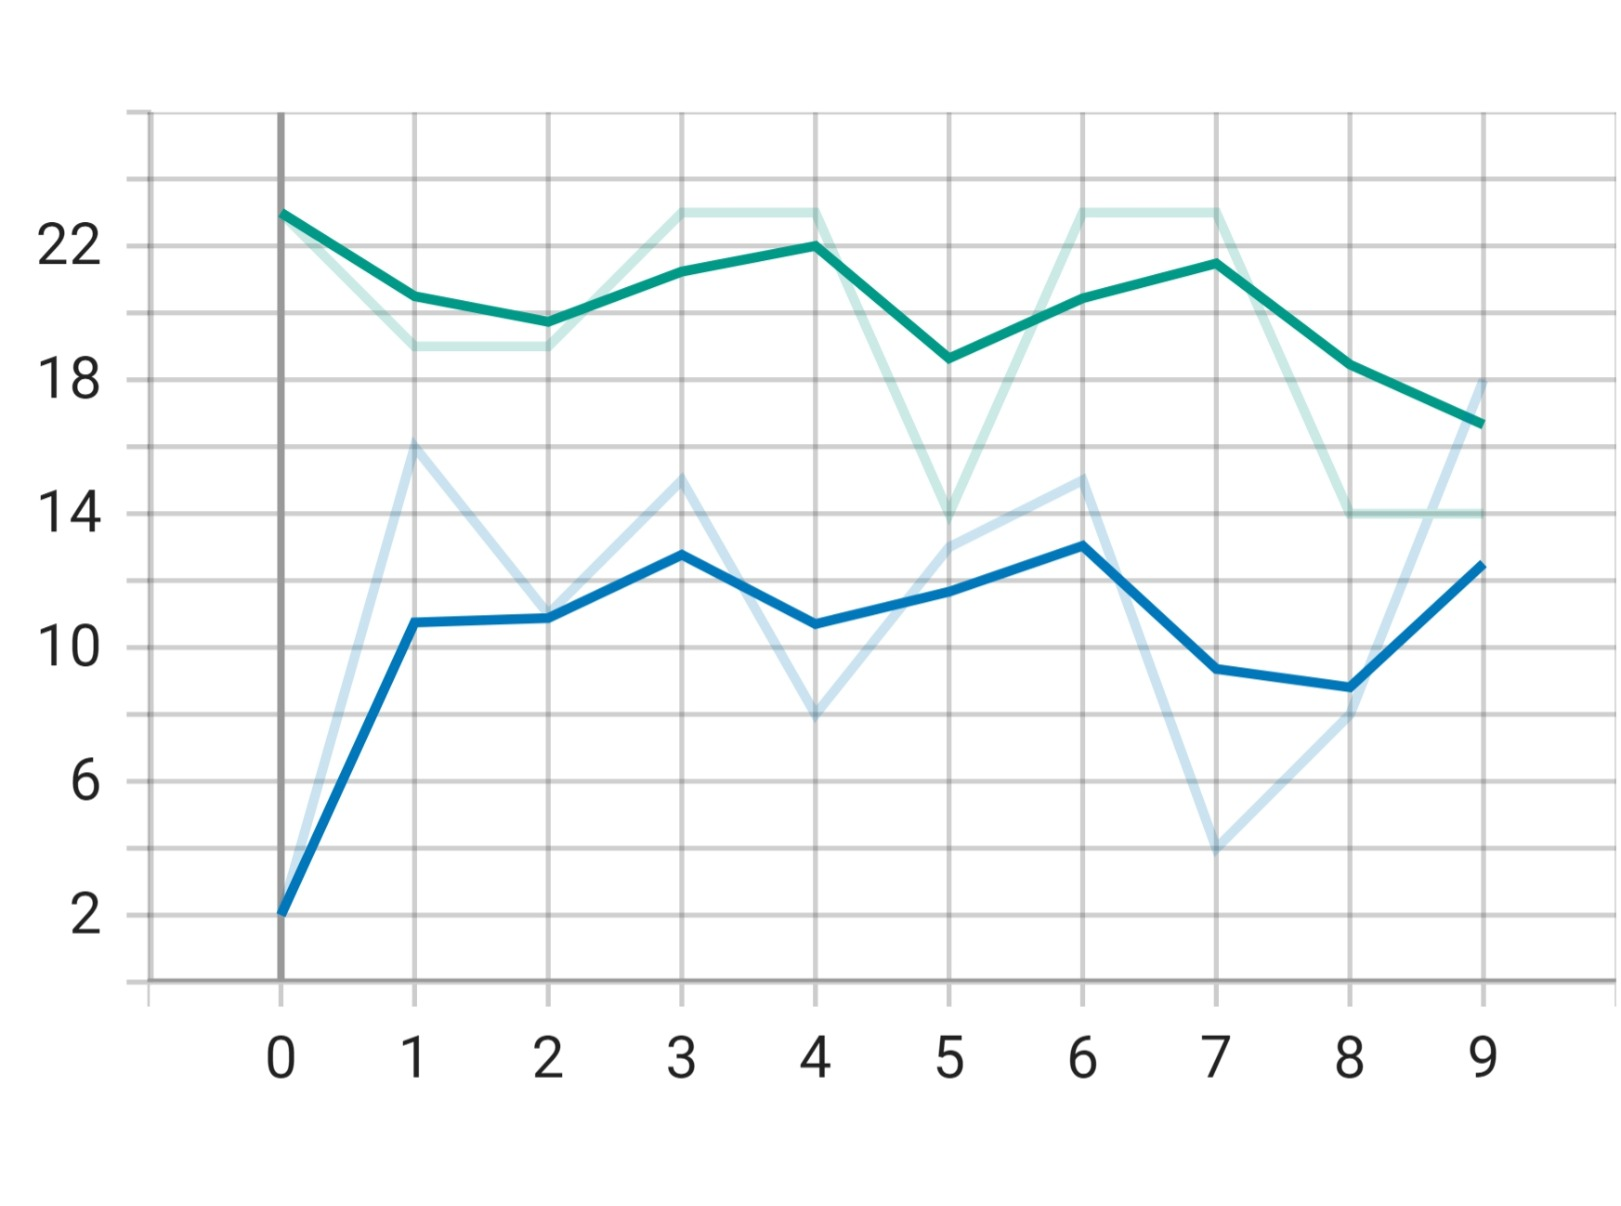
\includegraphics[width=.5\textwidth]{figures/sac/png/eval_episodic_return_deterministic_vs_stochastic.jpeg}
	\caption{The two possible SAC evaluation (deterministic in green and stochastic in blue) compared on Breakout. The plots show the 10 raw evaluation returns.}
	\label{fig:eval_episodic_return_deterministic_vs_stochastic}
\end{figure}

\paragraph{Observations}
\begin{itemize}
	\item \textbf{High Q-Function Variance:} Both QF1 and QF2 exhibit substantial spikes in losses and inflated value estimates, suggesting overestimation or instability in certain seeds—a common challenge in off-policy algorithms with limited training interactions.
	\item \textbf{$\alpha$ Behavior:} The learned entropy coefficient ($\alpha$) displays a U-shaped trajectory, initially decreasing to promote exploitation, then increasing in some runs (even exceeding 1.0), which indicates renewed exploration later in training.
	\item \textbf{Performance Skew:} Extremely poor performance in \emph{Boxing} dominates the human‐norm average, although environments like \emph{Breakout} and \emph{Assault} achieve moderate positive scores, illustrating the algorithm's uneven game-to-game performance in only 100k steps.
	\item \textbf{Emissions:} The relatively high number of gradient updates (the update frequency is set to 4), coupled with maintaining two critics/Q-functions, results in higher carbon emissions ($\sim$\num{0.01545}\,kg\,CO\textsubscript{2}) compared to simpler on-policy methods, although this is expected given the off-policy nature of SAC.
\end{itemize}

Overall, SAC shows promise in some Atari tasks under 100k interactions, yet it suffers from high variance in Q-function estimates and a complex $\alpha$ schedule. Longer training or adjustments to the critic updates (maybe more conservative ones) may be required to achieve more stable performance across seeds.

\subsection{Overall Comparison of Policy Gradient Algorithms}
\label{subsec:policy_comparison}
In this section, we compare the three policy gradient algorithms tested in our benchmark: \textbf{PPO} (on-policy with a clipped objective), \textbf{REINFORCE} (a basic Monte Carlo policy gradient), and \textbf{SAC} (an off-policy method with automatic entropy tuning). Each algorithm was trained for \num{100000} steps on the same 8 Atari games, with 4 random seeds per game, producing 32 runs per algorithm. We examine both their \emph{final performance} (human‐normalized and min–max normalized returns) and \emph{carbon emissions} over the course of training.

\paragraph{Final Evaluation Performance: Human‐Normalized.}
Table~\ref{tab:policy_final_eval_human} summarizes the aggregated human‐normalized returns over all 8 environments for each algorithm (mean, std, etc.). By this metric, PPO shows the highest mean value (\num{0.077}), albeit with large variance (\num{0.563}). \textbf{REINFORCE} follows at \num{0.026}, while SAC has a negative average (\num{-1.10}), strongly influenced by its very poor performance on \emph{Boxing} (see Section~\ref{subsubsec:sac} for details). Notably, the interquartile mean (IQM) for all three algorithms is near zero or slightly negative, reflecting that the short 100k‐step horizon yields limited gains in some games. SAC's extreme negative outliers in \emph{Boxing} pull its mean well below zero, even though it attains moderate success in \emph{Assault} and \emph{Breakout}.

\begin{table} 
	\centering
	\caption{Overall human‐normalized returns (aggregated) for policy gradient algorithms.}
	\label{tab:policy_final_eval_human}
	\begin{tabular}{lcccccc}
		\toprule
		\textbf{Algorithm} & \textbf{Mean} & \textbf{Std} & \textbf{Min} & \textbf{Max} & \textbf{IQM} & \textbf{Median} \\
		\midrule
		PPO         & 0.077 & 0.563 & -5.02 & 3.31 & 0.0173 & 0.0163 \\
		REINFORCE   & 0.026 & 0.355 & -2.40 & 2.83 & -0.0039 & -0.0029 \\
		SAC         & -1.100 & 4.428 & -23.36 & 0.93 & 0.0085 & 0.0045 \\
		\bottomrule
	\end{tabular}
\end{table}

\paragraph{Final Evaluation Performance: Min–Max Normalized.}
A similar pattern emerges when we switch to min–max normalization, as shown in Table~\ref{tab:policy_final_eval_minmax}. Here, \emph{PPO} leads with a mean of \num{0.248}, slightly outperforming \emph{SAC} (\num{0.227}). \emph{REINFORCE} remains lower on average (\num{0.154}). Interestingly, SAC's min–max maximum (\num{0.826}) is in line with PPO's (\num{0.964}), suggesting some of its runs achieve decent returns in certain games, offset by very low or zero returns in others.

\begin{table} 
	\centering
	\caption{Overall min--max normalized returns (aggregated) for policy gradient algorithms.}
	\label{tab:policy_final_eval_minmax}
	\begin{tabular}{lcccccc}
		\toprule
		\textbf{Algorithm} & \textbf{Mean} & \textbf{Std} & \textbf{Min} & \textbf{Max} & \textbf{IQM} & \textbf{Median} \\
		\midrule
		PPO         & 0.248 & 0.271 & 0.00 & 0.964 & 0.1523 & 0.1204 \\
		REINFORCE   & 0.154 & 0.252 & 0.00 & 0.853 & 0.0291 & 0.0393 \\
		SAC         & 0.227 & 0.254 & 0.00 & 0.826 & 0.1477 & 0.1105 \\
		\bottomrule
	\end{tabular}
\end{table}

\paragraph{Emissions and Energy Consumption.}
Figure~\ref{fig:policy_emissions_bar} shows the \textbf{carbon emissions} tracked during training (kg\,CO\textsubscript{2}\,eq), while Table~\ref{tab:policy_emissions} shows the mean emissions for each algorithm aggregated over all 32 runs. PPO exhibits the lowest emissions, averaging $\sim$\num{0.0029}\,kg\,CO\textsubscript{2}\,eq per run, whereas SAC is by far the highest ($\sim$\num{0.0154}\,kg). REINFORCE lands in the middle at $\sim$\num{0.0068}\,kg\,CO\textsubscript{2}\,eq. These differences likely arise from:
\begin{itemize}
	\item \emph{REINFORCE}: simpler architecture, but it replays from scratch each episode (Monte Carlo), incurring moderate overhead.  
	\item \emph{PPO}: on-policy sampling plus parallel environments yield a relatively fast throughput, reducing total compute time.  
	\item \emph{SAC}: off-policy approach with frequent gradient updates, two Q-networks, and autotuning overhead results in higher GPU usage.
\end{itemize}

\begin{table} 
	\centering
	\caption{Average carbon emissions (kg\,CO\textsubscript{2}\,eq) for policy gradient algorithms over 100k steps.}
	\label{tab:policy_emissions}
	\begin{tabular}{lcccc}
		\toprule
		\textbf{Algorithm} & \textbf{Mean} & \textbf{Std} & \textbf{Min} & \textbf{Max} \\
		\midrule
		PPO         & 0.00288 & 0.00039 & 0.00244 & 0.00369 \\
		REINFORCE   & 0.00676 & 0.00056 & 0.00614 & 0.00760 \\
		SAC         & 0.01545 & 0.00033 & 0.01495 & 0.01610 \\
		\bottomrule
	\end{tabular}
\end{table}

\begin{figure} 
	\centering
	\includesvg[width=0.5\textwidth]{figures/policy_comparison/barplot_emissions_policy_comparison}
	\caption{\emph{Policy Algorithms: Mean Emissions (kg\,CO\textsubscript{2}\,eq).} Error bars show the standard deviation across 32 runs.}
	\label{fig:policy_emissions_bar}
\end{figure}

\paragraph{Performance vs. Emissions}
Beyond the aggregated returns and raw carbon footprints, it is also informative to visualize the trade‐off between \emph{mean emissions} (kg\,CO\textsubscript{2}\,eq) and \emph{performance} (mean or IQM). Figures~\ref{fig:scatter_emissions_a} and \ref{fig:scatter_emissions_b} combine these metrics under both human and min–max normalization.

\begin{figure} 
	\centering
	\subfloat[\emph{IQM (Human)}]{%
		\includesvg[width=0.45\textwidth]{figures/policy_comparison/scatter_iqmean_human_policy_comparison}
		\label{fig:scatter_iqmean_human}
	}
	\quad
	\subfloat[\emph{IQM (Min--Max)}]{%
		\includesvg[width=0.45\textwidth]{figures/policy_comparison/scatter_iqmean_minmax_policy_comparison}
		\label{fig:scatter_iqmean_minmax}
	}
	\caption{\emph{Mean Emissions vs. Interquartile Mean (IQM) Return.}
		Each point corresponds to one algorithm's aggregated final performance (IQM) against its mean carbon emissions. 
		\textbf{(a)} uses human‐normalized returns, while \textbf{(b)} is min--max normalized.}
	\label{fig:scatter_emissions_a}
\end{figure}

\begin{figure} 
	\centering
	\subfloat[\emph{Mean (Human)}]{%
		\includesvg[width=0.45\textwidth]{figures/policy_comparison/scatter_mean_human_policy_comparison}
		\label{fig:scatter_mean_human}
	}
	\quad
	\subfloat[\emph{Mean (Min--Max)}]{%
		\includesvg[width=0.45\textwidth]{figures/policy_comparison/scatter_mean_minmax_policy_comparison}
		\label{fig:scatter_mean_minmax}
	}
	\caption{\emph{Mean Emissions vs. Mean Return.}
		Similar to Fig.~\ref{fig:scatter_emissions_a}, but plotting the average (mean) final performance in human \textbf{(a)} vs.\ min--max \textbf{(b)} normalization.}
	\label{fig:scatter_emissions_b}
\end{figure}

In all four scatter plots, PPO (blue) occupies the \emph{lowest emissions} regime (approximately \num{0.003}~kg\,CO\textsubscript{2}\,eq) yet achieves higher (or comparable) returns than the others. SAC (red) clearly emits more ($\approx$\num{0.015}~kg\,CO\textsubscript{2}\,eq), placing it on the far right of each scatter, while its performance can be strong (especially in mean min–max) or moderate (IQM), depending on the metric. REINFORCE (orange) sits in between for emissions ($\approx$ \num{0.007}~kg) but remains near zero or negative in human‐normalized returns.

Overall, these visualizations underscore a trade‐off: although SAC can sometimes compete in raw performance, its significantly higher carbon footprint may not be ideal for short 100k‐step benchmarks.

\paragraph{Training Throughput and Runtime}
A key factor driving these energy differences is \emph{training speed}, often measured in \emph{Samples per Second} (SPS). Figure~\ref{fig:policy_sps_comparison} compares the SPS curves for PPO, SAC, and REINFORCE across the 100k interactions. Meanwhile, Table~\ref{tab:policy_training_time} lists the total wall‐clock time for all 32 runs (8 games × 4 seeds).

\begin{figure} 
	\centering
	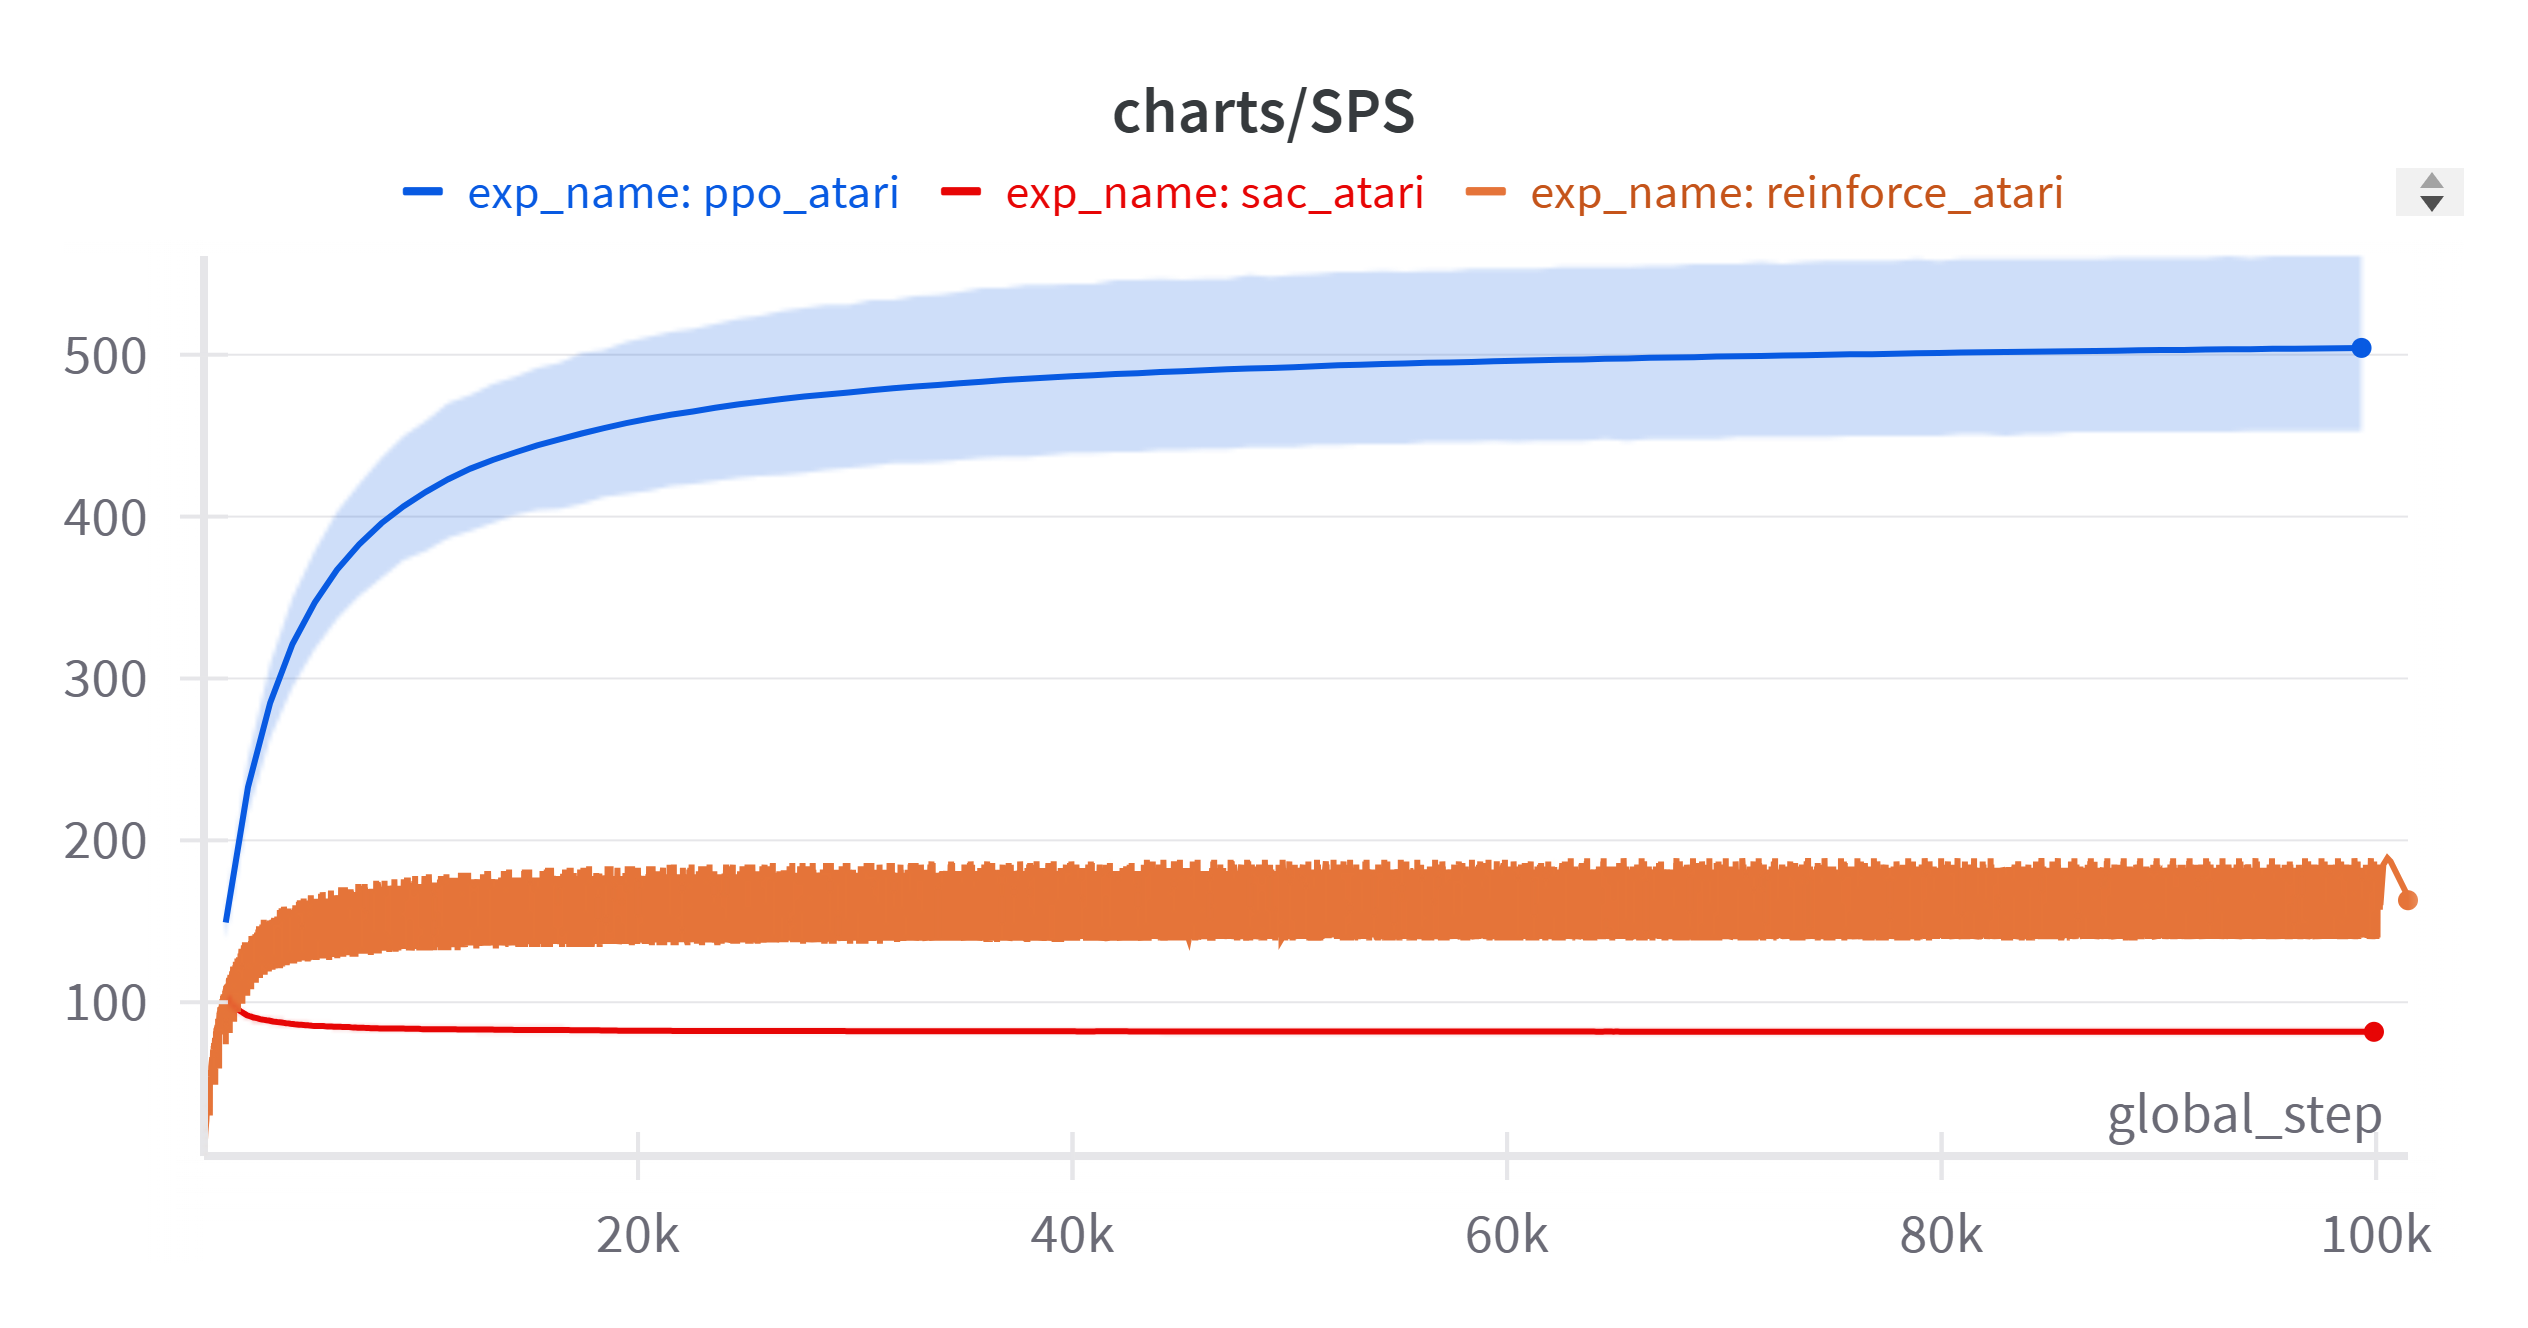
\includegraphics[width=0.6\textwidth]{figures/policy_comparison/policy_sps_comparison.png}
	\caption{\emph{Combined SPS curves for PPO, SAC, and REINFORCE.}
		PPO rapidly climbs above 400--500~SPS, while SAC settles around 100--120, and REINFORCE around 150--200. 
		Shaded areas (if visible) indicate min--max across seeds.}
	\label{fig:policy_sps_comparison}
\end{figure}

\begin{table} 
	\centering
	\caption{Total wall‐clock time for 32 runs (8 games × 4 seeds) per algorithm.}
	\label{tab:policy_training_time}
	\begin{tabular}{lc}
		\toprule
		\textbf{Algorithm} & \textbf{Total Training Time}\\
		\midrule
		PPO         & 2\,h 25\,m 08\,s \\
		REINFORCE   & 5\,h 53\,m 23\,s \\
		SAC         & 11\,h 28\,m 23\,s \\
		\bottomrule
	\end{tabular}
\end{table}

\emph{PPO} easily attains the highest SPS ($\sim$\num{500}), completing all runs in just over 2.4~hours. This efficiency helps keep its emissions the lowest.  
\emph{SAC}'s off‐policy updates and dual Q‐networks produce a low SPS ($\sim$\num{100}), causing an 11.5‐hour total runtime and the highest carbon footprint.  
\emph{REINFORCE}, despite simpler logic, often hits $\sim$\num{150}~SPS, finishing around 5.9~hours. Its overhead partly stems from lower data efficiency (Monte Carlo returns) and non‐parallel sampling.

\paragraph{Per-Game Observations}
To illustrate performance trends for PPO, REINFORCE, and SAC, each of the eight Atari games is now presented with a paired set of plots. One subfigure shows the human‐normalized returns over \num{100000} steps, while the other displays the corresponding returns under min--max normalization, which rescales each environment's returns based on its observed minimum and maximum. This dual presentation clarifies differences that might be obscured by large raw score ranges.

\medskip

\noindent \textbf{Alien.} Figure~\ref{fig:alien_combined} shows that the numeric range under min--max is larger (up to 0.14) than in human norm (up to 0.05), yet the relative ordering (PPO $\approx$ SAC > REINFORCE) remains similar.

\begin{figure} 
	\centering
	\subfloat[\emph{Human Norm}]{
		\includesvg[width=0.45\textwidth]{figures/policy_comparison/charts_episodic_return_human_comparison_AlienNoFrameskip-v4_policy}
		\label{fig:alien_human}
	}
	\quad
	\subfloat[\emph{Min--Max Norm}]{
		\includesvg[width=0.45\textwidth]{figures/policy_comparison/charts_episodic_return_minmax_comparison_AlienNoFrameskip-v4_policy}
		\label{fig:alien_minmax}
	}
	\caption{\emph{Alien.} 
		(\textbf{a}) Under human normalization, PPO (blue) and SAC (red) periodically reach 0.04--0.05, while REINFORCE (orange) lingers near 0.0.
		(\textbf{b}) Min--max scaling places PPO's peaks around 0.12--0.14, with SAC following closely by 100k steps, and REINFORCE near 0.04--0.08.}
	\label{fig:alien_combined}
\end{figure}

\medskip

\noindent \textbf{Amidar.} In Figure~\ref{fig:amidar_combined}, the difference is more dramatic in min--max space, where PPO nears 0.35 vs.\ $\approx$\num{0.05} in human norm.
\begin{figure} 
	\centering
	\subfloat[\emph{Human Norm}]{
		\includesvg[width=0.45\textwidth]{figures/policy_comparison/charts_episodic_return_human_comparison_AmidarNoFrameskip-v4_policy}
		\label{fig:amidar_human}
	}
	\quad
	\subfloat[\emph{Min--Max Norm}]{
		\includesvg[width=0.45\textwidth]{figures/policy_comparison/charts_episodic_return_minmax_comparison_AmidarNoFrameskip-v4_policy}
		\label{fig:amidar_minmax}
	}
	\caption{\emph{Amidar.}
		(\textbf{a}) PPO (blue) rises above 0.03, while SAC (red) and REINFORCE (orange) stay under 0.01. 
		(\textbf{b}) Min--max scaling reveals PPO crossing 0.30, whereas SAC/REINFORCE remain below 0.1.}
	\label{fig:amidar_combined}
\end{figure}

\medskip

\noindent \textbf{Assault.} PPO leads in both scales (Figure~\ref{fig:assault_combined}) with a clear margin, more easily readable under min--max (0.50 vs.\ 0.35).
\begin{figure} 
	\centering
	\subfloat[\emph{Human Norm}]{
		\includesvg[width=0.45\textwidth]{figures/policy_comparison/charts_episodic_return_human_comparison_AssaultNoFrameskip-v4_policy}
		\label{fig:assault_human_policy}
	}
	\quad
	\subfloat[\emph{Min--Max Norm}]{
		\includesvg[width=0.45\textwidth]{figures/policy_comparison/charts_episodic_return_minmax_comparison_AssaultNoFrameskip-v4_policy}
		\label{fig:assault_minmax_policy}
	}
	\caption{\emph{Assault.}
		(\textbf{a}) PPO (blue) approaches 0.15--0.18, while SAC (red) remains near 0.05--0.10.
		(\textbf{b}) Min--max scaling finds PPO around 0.30--0.50, SAC 0.20--0.35, and REINFORCE (orange) near 0.20--0.30.}
	\label{fig:assault_combined}
\end{figure}

\medskip

\noindent \textbf{Boxing.} Figure~\ref{fig:boxing_combined} highlights how an environment's large or small absolute score range can drastically alter the min--max scale.
\begin{figure} 
	\centering
	\subfloat[\emph{Human Norm}]{
		\includesvg[width=0.45\textwidth]{figures/policy_comparison/charts_episodic_return_human_comparison_BoxingNoFrameskip-v4_policy}
		\label{fig:boxing_human}
	}
	\quad
	\subfloat[\emph{Min--Max Norm}]{
		\includesvg[width=0.45\textwidth]{figures/policy_comparison/charts_episodic_return_minmax_comparison_BoxingNoFrameskip-v4_policy}
		\label{fig:boxing_minmax}
	}
	\caption{\emph{Boxing.}
		(\textbf{a}) All three exhibit wild swings in human norm (e.g., REINFORCE from -1.5 to +2).
		(\textbf{b}) Min--max compresses those swings to $\sim$\num{0.72}--\num{0.82}.}
	\label{fig:boxing_combined}
\end{figure}

\medskip

\noindent \textbf{Breakout.} In Breakout, \textbf{SAC} is the clear winner under both normalizations, though the gap appears even larger in min--max form.
\begin{figure} 
	\centering
	\subfloat[\emph{Human Norm}]{
		\includesvg[width=0.45\textwidth]{figures/policy_comparison/charts_episodic_return_human_comparison_BreakoutNoFrameskip-v4_policy}
		\label{fig:breakout_human}
	}
	\quad
	\subfloat[\emph{Min--Max Norm}]{
		\includesvg[width=0.45\textwidth]{figures/policy_comparison/charts_episodic_return_minmax_comparison_BreakoutNoFrameskip-v4_policy}
		\label{fig:breakout_minmax}
	}
	\caption{\emph{Breakout.}
		(\textbf{a}) SAC (red) surpasses 0.4--0.5, well above PPO (blue) or REINFORCE (orange).
		(\textbf{b}) Min--max confirms SAC reaching above 0.5, while PPO stays near 0.2.}
	\label{fig:breakout_combined}
\end{figure}

\medskip

\noindent \textbf{Freeway.} Figure~\ref{fig:freeway_combined} illustrates how SAC and REINFORCE barely register on either scale, as PPO's partial success reveals a bigger raw score gap.
\begin{figure} 
	\centering
	\subfloat[\emph{Human Norm}]{
		\includesvg[width=0.45\textwidth]{figures/policy_comparison/charts_episodic_return_human_comparison_FreewayNoFrameskip-v4_policy}
		\label{fig:freeway_human}
	}
	\quad
	\subfloat[\emph{Min--Max Norm}]{
		\includesvg[width=0.45\textwidth]{figures/policy_comparison/charts_episodic_return_minmax_comparison_FreewayNoFrameskip-v4_policy}
		\label{fig:freeway_minmax}
	}
	\caption{\emph{Freeway.}
		(\textbf{a}) PPO (blue) climbs to $\sim$\num{0.18}--\num{0.20}, while SAC (red) and REINFORCE (orange) remain near 0.0.
		(\textbf{b}) Min--max also shows PPO at $\sim$\num{0.20}, with the others near 0.0.}
	\label{fig:freeway_combined}
\end{figure}



\medskip

\noindent \textbf{MsPacman.} Figure~\ref{fig:mspacman_combined} underscores \textbf{PPO}'s lead in MsPacman, while SAC remains behind, and REINFORCE barely improves.
\begin{figure} 
	\centering
	\subfloat[\emph{Human Norm}]{
		\includesvg[width=0.45\textwidth]{figures/policy_comparison/charts_episodic_return_human_comparison_MsPacmanNoFrameskip-v4_policy}
		\label{fig:mspacman_human}
	}
	\quad
	\subfloat[\emph{Min--Max Norm}]{
		\includesvg[width=0.45\textwidth]{figures/policy_comparison/charts_episodic_return_minmax_comparison_MsPacmanNoFrameskip-v4_policy}
		\label{fig:mspacman_minmax}
	}
	\caption{\emph{MsPacman.}
		(\textbf{a}) PPO (blue) peaks near 0.08 by 80k steps, SAC (red) stays in 0.03--0.05, REINFORCE (orange) below 0.02.
		(\textbf{b}) Min--max scales these results, yielding PPO at $\sim$\num{0.35}--\num{0.40} vs.\ SAC $\sim$\num{0.15}--\num{0.20}, and REINFORCE < 0.10.}
	\label{fig:mspacman_combined}
\end{figure}



\medskip

\noindent \textbf{Pong.} In \emph{Pong}, Figure~\ref{fig:pong_combined} reveals no substantial improvement by PPO, SAC, or REINFORCE, regardless of the normalization scheme.
\begin{figure} 
	\centering
	\subfloat[\emph{Human Norm}]{
		\includesvg[width=0.45\textwidth]{figures/policy_comparison/charts_episodic_return_human_comparison_PongNoFrameskip-v4_policy}
		\label{fig:pong_human}
	}
	\quad
	\subfloat[\emph{Min--Max Norm}]{
		\includesvg[width=0.45\textwidth]{figures/policy_comparison/charts_episodic_return_minmax_comparison_PongNoFrameskip-v4_policy}
		\label{fig:pong_minmax}
	}
	\caption{\emph{Pong.}
		(\textbf{a}) All three methods fluctuate around 0.0--0.06 in human norm.
		(\textbf{b}) Min--max normalizes that to about 0.0--0.2.}
	\label{fig:pong_combined}
\end{figure}

\medskip

\noindent
\textbf{Overall Takeaways.}
Our analysis across both human‐normalized and min--max normalized returns reveals consistent trends among the three algorithms. Across all eight Atari games, \textbf{PPO} generally achieves the highest or near‐highest returns—especially in \emph{Amidar}, \emph{Assault}, \emph{Freeway}, and \emph{MsPacman}—demonstrating robust performance over the 100k‐step benchmark. In contrast, while \textbf{SAC} excels notably in \emph{Breakout} (and sometimes in \emph{Alien}), it exhibits greater variability, struggling in environments such as \emph{Freeway} and \emph{Pong} and showing high volatility in \emph{Boxing}. \textbf{REINFORCE} consistently underperforms, with only occasional spikes (as seen in \emph{Boxing}), which highlights the challenges of employing pure Monte Carlo policy gradients within this strongly limited interaction horizon.

Moreover, while the two normalization schemes yield different numerical scales—reflecting, for example, that large raw score ranges in \emph{Boxing} are compressed under min--max—the relative ranking among the algorithms remains largely similar. Overall, these findings underscore \textbf{PPO} as the most consistently successful policy gradient method in our study, with \textbf{SAC} showing pockets of promise amid higher variance, and \textbf{REINFORCE} trailing significantly in most tasks.

\paragraph{Synthesis}
Putting it all together:
\begin{itemize}
	\item \textbf{PPO} emerges as the most \emph{energy‐efficient} approach, yielding good (and sometimes top) performance while taking the shortest total runtime ($\approx$2.4h). It also leads in many environments, particularly \emph{Amidar}, \emph{Assault}, \emph{Freeway}, and \emph{MsPacman}.
	\item \textbf{SAC} can match or exceed PPO in certain tasks (\emph{Breakout}, \emph{Alien}), but suffers from a long training time and high emissions due to frequent gradient updates and dual Q‐networks. Its negative outliers in \emph{Boxing} also drag down the overall mean.
	\item \textbf{REINFORCE} sits in the middle for carbon usage ($\approx$\num{0.007}~kg\,CO\textsubscript{2}\,eq), but lags behind significantly in final returns, highlighting the difficulty of pure Monte Carlo methods within 100k steps.
\end{itemize}
Hence, for \emph{short‐horizon} Atari training, \textbf{PPO} stands out as the best balance of performance and sustainability, while \textbf{SAC} demands substantially more compute resources for often modest gains—except in specialized games like \emph{Breakout}, where it excels. 

\subsection{Overall Algorithm Comparison}
\label{subsec:overall_algo_comparison}

We now bring together all eight algorithms from our benchmark—five value-based methods 
(\emph{DQN, DDQN, DuelingDQN, PER, C51}) plus three policy-gradient methods 
(\emph{REINFORCE, PPO, SAC})—to provide a unified comparison of their final performance, 
carbon emissions, training runtime, and throughput (SPS).

\subsubsection{Final Evaluation Performance}

Tables~\ref{tab:all_algo_eval_human} and~\vref{tab:all_algo_eval_minmax} summarize the 
aggregated performance (mean, std, min, max, median, IQM) for each algorithm under both 
human and min--max normalization, respectively. These results extend 
the single-family comparisons made earlier to the full set of eight algorithms.

% --- Table of all 8 algorithms: human norm
\begin{table} 
	\centering
	\caption{Overall final returns (human‐normalized) for all algorithms.}
	\label{tab:all_algo_eval_human}
	\begin{tabular}{lcccccc}
		\toprule
		\textbf{Algorithm} & \textbf{Mean} & \textbf{Std} & \textbf{Min} & \textbf{Max} & \textbf{IQM} & \textbf{Median} \\
		\midrule
		C51       & -1.0811 & 3.2862 & -12.88 & 0.7770 & 0.0068 & 0.0000 \\
		DDQN      & 0.0226  & 1.0083 & -8.5952 & 2.5952 & 0.0894 & 0.0527 \\
		DQN       & 0.1353  & 0.7541 & -5.0238 & 4.7381 & 0.1137 & 0.0338 \\
		DUELING\_DQN & 0.1860  & 0.5258 & -1.9286 & 3.5476 & 0.1020 & 0.0402 \\
		PER       & 0.0607  & 1.0170 & -10.2619 & 6.8809 & 0.0813 & 0.0539 \\
		PPO       & 0.0775  & 0.5632 & -5.0238 & 3.3095 & 0.0173 & 0.0163 \\
		REINFORCE & 0.0259  & 0.3549 & -2.4048 & 2.8333 & -0.0039 & -0.0029 \\
		SAC       & -1.1000 & 4.4278 & -23.3571 & 0.9286 & 0.0085 & 0.0045 \\
		\bottomrule
	\end{tabular}
\end{table}

% --- Table of all 8 algorithms: minmax norm
\begin{table} 
	\centering
	\caption{Overall final returns (min--max normalized) for all algorithms.}
	\label{tab:all_algo_eval_minmax}
	\begin{tabular}{lcccccc}
		\toprule
		\textbf{Algorithm} & \textbf{Mean} & \textbf{Std} & \textbf{Min} & \textbf{Max} & \textbf{IQM} & \textbf{Median} \\
		\midrule
		C51       & 0.2503 & 0.2568 & 0.0 & 0.8270 & 0.1400 & 0.2005 \\
		DDQN      & 0.3737 & 0.2854 & 0.0 & 1.0000 & 0.3272 & 0.2887 \\
		DQN       & 0.3802 & 0.3099 & 0.0 & 0.9881 & 0.3426 & 0.2899 \\
		DUELING\_DQN & 0.3849 & 0.3056 & 0.0 & 0.9523 & 0.3454 & 0.2632 \\
		PER       & 0.3533 & 0.2695 & 0.0 & 0.9845 & 0.3087 & 0.2583 \\
		PPO       & 0.2481 & 0.2712 & 0.0 & 0.9643 & 0.1523 & 0.1204 \\
		REINFORCE & 0.1544 & 0.2515 & 0.0 & 0.8527 & 0.0291 & 0.0393 \\
		SAC       & 0.2272 & 0.2536 & 0.0 & 0.8258 & 0.1477 & 0.1105 \\
		\bottomrule
	\end{tabular}
\end{table}

From these tables, we see that among the \emph{value-based} algorithms, 
Dueling DQN, DQN, and Double DQN often exhibit the highest mean or IQM returns, while 
\emph{PER} and \emph{C51} sometimes trail behind or show higher variance (especially in 
human‐norm with large negative outliers). For the \emph{policy gradient} group, SAC yields strong 
results in some tasks but is heavily penalized in others (e.g., \emph{Boxing}), resulting 
in negative or near‐zero means in human norm. PPO remains moderate, whereas REINFORCE 
lags in final average.

\subsubsection{Emissions and Runtime}

Figure~\ref{fig:barplot_emissions_total} compares the average emissions (kg\,CO\textsubscript{2}\,eq) for 
all 8 algorithms, along with standard deviation error bars. Table~\ref{tab:total_runtimes} 
then lists each method's total wall‐clock time to complete 8 games × 4 seeds = 32 runs.

The total training times of the algorithms are critical from a practical deployment perspective. As Table~\ref{tab:total_runtimes} indicates, PPO completes the 32 runs in only 2.4 hours, which not only minimizes energy consumption but also enables rapid prototyping and iterative tuning. In contrast, SAC's extended runtime of over 11 hours may hinder its use in scenarios where computational resources or time are limited—even if its performance is competitive on select tasks. The intermediate training times of the DQN-based variants (roughly 5–7 hours) suggest that they strike a balance between performance and efficiency. Therefore, when selecting a DRL algorithm, one must consider not only the final performance and energy efficiency but also the training time, which directly affects resource allocation and time-to-deployment.

\begin{figure} 
	\centering
	\includesvg[width=0.65\textwidth]{figures/comparison/barplot_emissions_total}
	\caption{\emph{Mean Emissions for All 8 Algorithms}, with standard deviation bars.
		SAC stands out at nearly 0.015~kg\,CO\textsubscript{2}\,eq on average, while PPO is notably lower than
		any of the DQN-based methods.}
	\label{fig:barplot_emissions_total}
\end{figure}

\begin{table} 
	\centering
	\caption{Total runtime (hh:mm:ss) over 32 runs per algorithm.}
	\label{tab:total_runtimes}
	\begin{tabular}{lc}
		\toprule
		\textbf{Algorithm} & \textbf{Total Time} \\
		\midrule
		DQN          & 5h 46m 54s \\
		DDQN         & 5h 55m 17s \\
		PER          & 6h 26m 58s \\
		DUELING\_DQN & 6h 08m 02s \\
		C51          & 6h 51m 23s \\
		REINFORCE    & 5h 53m 23s \\
		PPO          & 2h 25m 08s \\
		SAC          & 11h 28m 23s \\
		\bottomrule
	\end{tabular}
\end{table}

Emissions and runtime are clearly connected, in particular putting them together some key findings are:
\begin{itemize}
	\item SAC demands the longest runtime (over 11.4 hours) and, as seen in 
	Figure~\ref{fig:barplot_emissions_total}, produces the highest average emissions. 
	\item PPO completes all runs in just 2.4 hours, with the lowest \(\sim0.003\) 
	kg\,CO\textsubscript{2}\,eq. 
	\item Most DQN variants cluster around 5--7 hours total, with emissions 
	\(\sim0.006\)--0.008 kg\,CO\textsubscript{2}\,eq, well above PPO but significantly below SAC.
\end{itemize}

Finally, a comprehensive comparison of the algorithms' performance and energy consumption is presented in Table~\ref{tab:all_algorithms_summary}. This table compiles the key performance metrics—final evaluation mean, median, and interquartile mean (IQM) returns under both human-normalized and min-max normalized scales—along with the mean carbon emissions (in kg\,CO\textsubscript{2}\,eq) for each algorithm, providing a holistic overview of their respective trade-offs.

\begin{table}
	\centering
	\caption{Final Evaluation Returns and Emissions for All Algorithms}
	\label{tab:all_algorithms_summary}
	\footnotesize % Reduce font size to fit more columns
	\makebox[\textwidth]{%
	\begin{tabular}{l
			S[table-format=1.3]
			S[table-format=1.3]
			S[table-format=1.3]
			S[table-format=1.3]
			S[table-format=1.3]
			S[table-format=1.3]
			S[table-format=1.3e-3]
		}
		\toprule
		\textbf{Algorithm} & \multicolumn{3}{c}{\textbf{Human-Normalized Return}} & \multicolumn{3}{c}{\textbf{Min-Max Normalized Return}} & {\textbf{Mean Emissions}} \\
		& {Mean} & {Median} & {IQM} & {Mean} & {Median} & {IQM} & {(kg\,CO\textsubscript{2}\,eq)} \\
		\midrule
		DQN         & 0.135 & 0.034 & 0.114 & 0.380 & 0.290 & 0.343  & 6.47e-3 \\
		Double DQN  & 0.023 & 0.053 & 0.089 & 0.374 & 0.289 & 0.327  & 6.67e-3 \\
		Prioritized ER& 0.061 & 0.054 & 0.081 & 0.353 & 0.258 & 0.309  & 7.25e-3 \\
		Dueling DQN & 0.186 & 0.040 & 0.102 & 0.385 & 0.263 & 0.345  & 6.89e-3 \\
		C51         & -1.081& 0.000 & 0.007 & 0.250 & 0.201 & 0.140  & 7.75e-3 \\
		REINFORCE   & 0.026 & -0.003 & -0.004& 0.154 & 0.039 & 0.029   & 6.76e-3 \\
		PPO         & 0.077 & 0.016 & 0.017 & 0.248 & 0.120 & 0.152   & 2.88e-3 \\
		SAC         & -1.100& 0.004 & 0.009 & 0.227 & 0.111 & 0.148   & 1.55e-2\\
		\bottomrule
	\end{tabular}
	}
\end{table}

\subsubsection{Steps per Second (SPS) Comparison}
Another measure of algorithmic efficiency is how many environment interactions each method 
can process per second. Figure~\ref{fig:sps_all} plots the aggregated SPS curves for all 
eight algorithms over 100k steps.

\begin{figure} 
	\centering
	\includesvg[width=0.65\textwidth]{figures/comparison/sps_all}
	\caption{\emph{SPS Comparison for all algorithms}. PPO (blue line/shade) surpasses 
		500 SPS (mainly due to the parallel environments), while DQN variants group around 150--200, REINFORCE near 150, and SAC remains 
		under 100. Shaded regions represent min--max across seeds.}
	\label{fig:sps_all}
\end{figure}

PPO quickly ramps up to $\sim500$~SPS, dwarfing the $\sim100$--200 range of the DQN 
algorithms plus REINFORCE. 
SAC, consistent with its high runtime/emissions, lingers around 80--100~SPS. 
Minor differences exist among the DQN variants (e.g., PER may have a slightly heavier overhead 
due to priority calculations, etc.).

\subsubsection{Performance vs. Emissions (Scatter Plots)}
To visualize how each algorithm trades off \emph{emissions} and \emph{performance},
we plot the \textit{mean carbon footprint} (\textit{x}-axis) against final evaluation 
(\textit{y}-axis). Figures~\ref{fig:scatter_all_iqmean} and~\ref{fig:scatter_all_mean}
each contain two subplots, one for \textit{human‐normalized} and one for 
\textit{min--max normalized} performance. We show both \textit{IQM} (i.e.\ interquartile mean) 
and \textit{mean} returns in separate figures.

\begin{figure} 
	\centering
	\subfloat[\textit{IQM (Human)}]{
		\includesvg[width=0.45\textwidth]{figures/comparison/scatter_iqmean_human_comparison}
		\label{fig:scatter_all_iqmean_human}
	}
	\quad
	\subfloat[\textit{IQM (Min--Max)}]{
		\includesvg[width=0.45\textwidth]{figures/comparison/scatter_iqmean_minmax_comparison}
		\label{fig:scatter_all_iqmean_minmax}
	}
	\caption{Mean Emissions vs.\ IQM Evaluation for All 8 Algorithms.
		\textbf{(a)} Human‐normalized IQM vs.\ mean emissions. 
		\textbf{(b)} Min--max–normalized IQM vs.\ mean emissions. 
		Points are labeled by algorithm (\texttt{c51, ddqn, dqn, dueling\_dqn, per, ppo, reinforce, sac}).}
	\label{fig:scatter_all_iqmean}
\end{figure}

\begin{figure} 
	\centering
	\subfloat[\textit{Mean (Human)}]{
		\includesvg[width=0.45\textwidth]{figures/comparison/scatter_mean_human_comparison}
		\label{fig:scatter_all_mean_human}
	}
	\quad
	\subfloat[\textit{Mean (Min--Max)}]{
		\includesvg[width=0.45\textwidth]{figures/comparison/scatter_mean_minmax_comparison}
		\label{fig:scatter_all_mean_minmax}
	}
	\caption{Mean Emissions vs.\ Mean Evaluation for All 8 Algorithms.
		\textit{(a)} Human‐normalized mean returns vs.\ emissions. 
		\textit{(b)} Min--max normalized mean returns vs.\ emissions.}
	\label{fig:scatter_all_mean}
\end{figure}

Across these four plots:
\begin{itemize}
	\item \textbf{PPO} (blue point) sits at the far left (\(\approx 0.003\) kg\,CO\textsubscript{2}\,eq), 
	with moderate returns in both IQM and mean. It is the most \emph{energy-efficient}.
	\item \textbf{SAC} (red point) is the rightmost outlier (\(\approx 0.015\)–0.016 kg\,CO\textsubscript{2}\,eq), 
	with widely varying performance depending on the metric. 
	\item \textbf{DQN-based variants} (C51 in pink, DDQN in red, DQN in gold,
	Dueling\_DQN in dark blue, PER in green) cluster in the \(\sim0.006\)--0.008 range
	of mean emissions. Some, e.g.\ \emph{DQN} or \emph{DuelingDQN}, achieve higher 
	IQM or mean than others.
	\item \textbf{REINFORCE} (orange) lies around \(\sim0.007\) emissions but yields 
	relatively low returns under both human‐norm and min–max.
\end{itemize}
Overall, these scatter plots underscore that \textit{PPO} provides a strong balance of 
moderate/high returns with minimal carbon cost, while \textit{SAC} can yield decent 
scores but at a high energy expense. The DQN-family methods vary: some (like 
Dueling DQN) approach or exceed PPO's performance, but typically with 2--3 times the emissions.

\subsubsection{Per-Environment Episodic Returns (All Algorithms)}
\label{sssec:per_env_all}

To better understand how each algorithm performs on individual Atari environments,
in this section we display the over-time training curves (up to 100k steps) for 
\emph{all eight} algorithms on each of the eight Atari environments under study, 
using both \textit{min--max} and \textit{human} normalization for the episodic returns. 
We discuss notable patterns in each environment below.

%------------------ ALIEN ------------------
\paragraph{AlienNoFrameskip-v4}
(Figure~\ref{fig:alien_comparison_combined})
\texttt{DDQN} (red) and \texttt{DQN} (gold) often spike above 0.15--0.20 in min--max, 
whereas \texttt{PPO} (blue) remains near 0.10--0.15. 
\texttt{SAC} (dark red) lingers lower but sometimes climbs late, 
\texttt{REINFORCE} (orange) generally stays near the bottom, and \texttt{C51} (pink) 
shows moderate oscillations. 
Under human norm, the range compresses to near 0.0--0.1 for many runs.

\begin{figure} 
	\centering
	\subfloat[\emph{Min--Max Norm}]{
		\includesvg[width=0.45\textwidth]{figures/comparison/charts_episodic_return_comparison_AlienNoFrameskip-v4}%
		\label{fig:alien_comparison_minmax}
	}
	\quad
	\subfloat[\emph{Human Norm}]{
		\includesvg[width=0.45\textwidth]{figures/comparison/charts_episodic_return_human_comparison_AlienNoFrameskip-v4}%
		\label{fig:alien_comparison_human}
	}
	\caption{\emph{Alien:} Episodic returns for C51 (pink), DDQN (red), 
		DQN (gold), DUELING DQN (dark blue), PER (green),
		PPO (navy blue), REINFORCE (orange), and SAC (dark red).}
	\label{fig:alien_comparison_combined}
\end{figure}

%------------------ AMIDAR ------------------
\paragraph{AmidarNoFrameskip-v4}
(Figure~\ref{fig:amidar_comparison_combined})
\texttt{DDQN} (red) and \texttt{Dueling\_DQN} (dark blue) surpass 0.4--0.5 near 80k steps 
in the min--max figure, while \texttt{C51} (pink) occasionally peaks around 0.5. 
\texttt{PPO} (blue) is more steady, around 0.2--0.3. \texttt{SAC} (dark red) 
and \texttt{REINFORCE} (orange) stay below 0.1. 
Under human norm, the overall scale is 0.0--0.06 for most algorithms, 
revealing smaller raw rewards in Amidar.

\begin{figure} 
	\centering
	\subfloat[\emph{Min--Max Norm}]{
		\includesvg[width=0.45\textwidth]{figures/comparison/charts_episodic_return_comparison_AmidarNoFrameskip-v4}%
		\label{fig:amidar_comparison_minmax}
	}
	\quad
	\subfloat[\emph{Human Norm}]{
		\includesvg[width=0.45\textwidth]{figures/comparison/charts_episodic_return_human_comparison_AmidarNoFrameskip-v4}%
		\label{fig:amidar_comparison_human}
	}
	\caption{\emph{Amidar:} Episodic returns across 100k steps.}
	\label{fig:amidar_comparison_combined}
\end{figure}

%------------------ ASSAULT ------------------
\paragraph{AssaultNoFrameskip-v4}
(Figure~\ref{fig:assault_comparison_combined})
\texttt{Dueling\_DQN} (dark blue) and \texttt{DQN} (gold) climb toward 0.8--0.85 
late in training (min--max). 
\texttt{PPO} (blue) approaches 0.7, while \texttt{reinforce} (orange) remains 
under 0.4. \texttt{C51} (pink) gradually ascends but ends around 0.6. 
Under human norm, the spread condenses between 0.0 and 0.4, consistent with higher 
raw scores in this environment.

\begin{figure} 
	\centering
	\subfloat[\emph{Min--Max Norm}]{
		\includesvg[width=0.45\textwidth]{figures/comparison/charts_episodic_return_comparison_AssaultNoFrameskip-v4}%
		\label{fig:assault_minmax}
	}
	\quad
	\subfloat[\emph{Human Norm}]{
		\includesvg[width=0.45\textwidth]{figures/comparison/charts_episodic_return_human_comparison_AssaultNoFrameskip-v4}%
		\label{fig:assault_human}
	}
	\caption{\emph{Assault:} Episodic returns across 100k steps.}
	\label{fig:assault_comparison_combined}
\end{figure}

%------------------ BOXING ------------------
\paragraph{BoxingNoFrameskip-v4}
(Figure~\ref{fig:boxing_comparison_combined})
Min--max values bunch around 0.5--0.8, with \texttt{DDQN} (red) sometimes near 0.8. 
\texttt{C51} (pink) hovers ~0.55--0.65. Meanwhile, in human norm, 
\texttt{C51} and \texttt{Reinforce} see large negative dips below -5.0, 
showing how Boxing's limited raw score range drastically affects the human scale. 
\texttt{PPO} (blue) and \texttt{Dueling\_DQN} (dark blue) stay near 0.0--1.0 
in that scale.

\begin{figure} 
	\centering
	\subfloat[\emph{Min--Max Norm}]{
		\includesvg[width=0.45\textwidth]{figures/comparison/charts_episodic_return_comparison_BoxingNoFrameskip-v4}%
		\label{fig:boxing_comparison_minmax}
	}
	\quad
	\subfloat[\emph{Human Norm}]{
		\includesvg[width=0.45\textwidth]{figures/comparison/charts_episodic_return_human_comparison_BoxingNoFrameskip-v4}%
		\label{fig:boxing_comparison_human}
	}
	\caption{\emph{Boxing:} Episodic returns across 100k steps.}
	\label{fig:boxing_comparison_combined}
\end{figure}

%------------------ BREAKOUT ------------------
\paragraph{BreakoutNoFrameskip-v4}
(Figure~\ref{fig:breakout_comparison_combined})
\texttt{SAC} (dark red) excels around 60k--100k steps, surpassing 0.5 in min--max 
and ~0.4--0.5 in human norm. \texttt{PPO} (blue) lags near 0.2, and \texttt{DQN} (gold) 
settles around 0.2--0.3. 
\texttt{Reinforce} (orange) stays near or below 0.1. 
Breakout highlights \emph{SAC}'s potential for strong late-game performance, 
albeit at a higher computational cost (\S\ref{subsec:overall_algo_comparison}).
\begin{figure} 
	\centering
	\subfloat[\emph{Min--Max Norm}]{
		\includesvg[width=0.45\textwidth]{figures/comparison/charts_episodic_return_comparison_BreakoutNoFrameskip-v4}%
		\label{fig:breakout_comparison_minmax}
	}
	\quad
	\subfloat[\emph{Human Norm}]{
		\includesvg[width=0.45\textwidth]{figures/comparison/charts_episodic_return_human_comparison_BreakoutNoFrameskip-v4}%
		\label{fig:breakout_comparison_human}
	}
	\caption{\emph{Breakout:} Episodic returns across 100k steps.}
	\label{fig:breakout_comparison_combined}
\end{figure}

%------------------ FREEWAY ------------------
\paragraph{FreewayNoFrameskip-v4}
(Figure~\ref{fig:freeway_comparison_combined})
Here, \texttt{DDQN} (red) rapidly climbs to 0.85+ in min--max by ~15k steps, 
with \texttt{C51} (pink) and \texttt{DQN} (gold) following suit. 
\texttt{PPO} (blue) only reaches ~0.6, 
\texttt{PER} (green) hits ~0.3, while \texttt{Reinforce} (orange) and \texttt{SAC} (dark red) 
remain near 0.0. 
In human norm, these large raw scores translate to 0.3--0.8 for the top algorithms, 
reflecting that Freeway has a high reward potential even early in training.
\begin{figure} 
	\centering
	\subfloat[\emph{Min--Max Norm}]{
		\includesvg[width=0.45\textwidth]{figures/comparison/charts_episodic_return_comparison_FreewayNoFrameskip-v4}%
		\label{fig:freeway_comparison_minmax}
	}
	\quad
	\subfloat[\emph{Human Norm}]{
		\includesvg[width=0.45\textwidth]{figures/comparison/charts_episodic_return_human_comparison_FreewayNoFrameskip-v4}%
		\label{fig:freeway_comparison_human}
	}
	\caption{\emph{Freeway:} Episodic returns across 100k steps.}
	\label{fig:freeway_comparison_combined}
\end{figure}

%------------------ MS PAC-MAN ------------------
\paragraph{MsPacmanNoFrameskip-v4}
(Figure~\ref{fig:mspacman_comparison_combined})
No single algorithm dominates strongly, but \texttt{dqn} (gold) and \texttt{ddqn} (red) 
occasionally spike above 0.25 in min--max, while \texttt{reinforce} (orange) remains 
near 0.0--0.1. \texttt{PPO} (blue) hovers around 0.15--0.20, 
with \texttt{c51} (pink) also in that range. 
Under human norm, the entire scale is fairly tight (~0.0--0.08) 
due to MsPacman's moderate raw reward potential within 100k steps.

\begin{figure} 
	\centering
	\subfloat[\emph{Min--Max Norm}]{
		\includesvg[width=0.45\textwidth]{figures/comparison/charts_episodic_return_comparison_MsPacmanNoFrameskip-v4}%
		\label{fig:mspacman_comparison_minmax}
	}
	\quad
	\subfloat[\emph{Human Norm}]{
		\includesvg[width=0.45\textwidth]{figures/comparison/charts_episodic_return_human_comparison_MsPacmanNoFrameskip-v4}%
		\label{fig:mspacman_comparison_human}
	}
	\caption{\emph{MsPacman:} Episodic returns across 100k steps.}
	\label{fig:mspacman_comparison_combined}
\end{figure}

%------------------ PONG ------------------
\paragraph{PongNoFrameskip-v4}
(Figure~\ref{fig:pong_comparison_combined})
\texttt{PER} (green) occasionally spikes near 0.3--0.4 in min--max, 
\texttt{DQN} (gold) has mid-range fluctuations, 
\texttt{PPO} (blue) and \texttt{Reinforce} (orange) remain under 0.2 for most runs. 
\texttt{SAC} (dark red) never climbs above 0.1. 
Because Pong's raw scoring can be small or negative, 
the human norm figure is mostly 0.0--0.1. None of the algorithms achieve 
the large positive returns that DQN-based methods have historically 
reached with much longer training.

\begin{figure} 
	\centering
	\subfloat[\emph{Min--Max Norm}]{
		\includesvg[width=0.45\textwidth]{figures/comparison/charts_episodic_return_comparison_PongNoFrameskip-v4}%
		\label{fig:pong_comparison_minmax}
	}
	\quad
	\subfloat[\emph{Human Norm}]{
		\includesvg[width=0.45\textwidth]{figures/comparison/charts_episodic_return_human_comparison_PongNoFrameskip-v4}%
		\label{fig:pong_comparison_human}
	}
	\caption{\emph{Pong:} Episodic returns across 100k steps.}
	\label{fig:pong_comparison_combined}
\end{figure}

\paragraph{Summary of Environment-Level Comparisons}
These per-environment plots reinforce the observations from our aggregate metrics.
Notable highlights:
\begin{itemize}
	\item \textbf{Freeway}: Some DQN variants (DDQN, DQN) rapidly approach near-maximum 
	scores, overshadowing \texttt{PPO} and \texttt{SAC}.
	\item \textbf{Breakout}: \texttt{SAC} outperforms others late in training.
	\item \textbf{Boxing}: Min--max compression vs.\ large negative swings in human norm 
	accentuates how the raw score range shapes these normalizations.
	\item \textbf{Amidar, Assault, Alien}: DuelingDQN and DQN often do well, 
	while \texttt{PPO} is typically moderate, and \texttt{SAC} or \texttt{Reinforce} 
	can lag behind.
\end{itemize}
Overall, each game's reward structure significantly influences how algorithms evolve 
over 100k steps, corroborating the broader performance–emissions findings in 
Section~\ref{subsec:overall_algo_comparison}.

\subsubsection{Summary}
Bringing all eight algorithms together reveals distinct trade‐offs among performance, 
emissions, and runtime:
\begin{itemize}
	\item \textbf{PPO} remains the overall most energy-efficient method, 
	finishing runs $\sim2.4$h total. Its final returns are decent, though 
	certain DQN variants can match or exceed it in specific tasks.
	\item \textbf{SAC} can excel (e.g.\ \emph{Breakout}) but has the highest 
	emissions and slowest SPS, taking over 11h to finish.
	\item \textbf{DQN-based variants} occupy a middle ground in both carbon 
	footprint ($\sim0.006$--0.008 kg\,CO\textsubscript{2}\,eq) and total runtime (5--7h). 
	Some, like Dueling DQN, achieve strong mean returns.
	\item \textbf{REINFORCE} similarly runs about 6h total, but yields lower 
	performance than DQN methods or PPO in most tasks.
\end{itemize}
Hence, if one's priority is \emph{high performance} but with minimal compute cost, 
\textbf{PPO} or select DQN variants might be ideal. \textbf{SAC} offers potential 
but requires significantly more energy for short 100k-step training. These findings 
highlight a clear \emph{trade‐off} between performance and sustainability. 
\textbf{PPO} is the most energy-efficient overall, while certain DQN variants can 
overtake it in raw performance yet emit 2--3$\times$ more CO\textsubscript{2}\,eq. \textbf{SAC} 
incurs the greatest overhead, offset by its strengths in a few tasks like 
\emph{Breakout}. In Section~\ref{sec:implications_results}, we discuss the broader 
implications of these results for real-world deployments and future research directions.

	\section{Implications of the Results}
\label{sec:implications_results}
This section interprets the findings from the previous section and discusses their broader implications.

This section is more interpretative and application-focused—it explains why the results matter.


\subsection{General Observations}
\begin{itemize}
	\item What trends emerged from the results?
	\item Were any algorithms unexpectedly energy-efficient?
	\item Did any algorithm perform significantly worse than expected in terms of energy usage?	
\end{itemize}
What were the most notable trends in the results?
Any surprising findings? (e.g., did a simpler method turn out to be more efficient than an advanced one?).

\subsection{Energy Efficiency vs. Performance Trade-Off}
\begin{itemize}
	\item Which algorithms achieved the best performance at low energy costs?
	\item Are high-performance methods necessarily more energy-intensive?
	\item Is there a clear "sweet spot" balancing energy and reward?
	\item Are there diminishing returns for performance improvements vs. energy consumption?
\end{itemize}
Which algorithms performed well at low energy costs?
Which algorithms achieved the best performance but at high energy costs?
Is there a clear “sweet spot” algorithm?

\subsection{Practical Implications for AI Sustainability}
\begin{itemize}
	\item If a company prioritizes high performance, which algorithm should they use?
	\item If low energy consumption is the main concern, what is the best choice?
	\item How can reinforcement learning be made more sustainable?
\end{itemize}
If companies want maximum performance, which algorithm should they choose?
If a low-carbon footprint is the priority, what’s the best option?
What does this study suggest about future AI energy efficiency research?
Seconda versione, dopo aver fatto notare della sezione conclusioni:
\begin{itemize}
	\item Which algorithms should be prioritized in resource-limited environments?
	\item If reinforcement learning is applied in an industry setting, which method should be chosen for:
	\begin{itemize}
		\item Maximum efficiency?
		\item Best performance at a reasonable cost?
		\item Low-carbon AI initiatives?
	\end{itemize}
	\item How could energy-efficient reinforcement learning impact research and business decisions?
\end{itemize}
---------
ricorda video su "deepseek clone at 30\$", dice tipo che quale algo usi sembra non fare differenza, quindi si potrebbe optare a prescindere per il più green, o soft spot tra reinforce e ppo per dire, magari reinforce with baseline e migliori batch.

\subsection{Limitations and Future Work}
(dopo lo slash la versione aggiornata dopo aver fatto notare che c'è la sezione conclusioni, la versione aggiornata delle direzioni future è semplicemente azzeccata dopo quella originale, nel senso primi due item sono vecchi, altri 3 nuovi)
\begin{itemize}
	\item \textbf{CodeCarbon limitations:} Real-time tracking slowed down experiments. / Real-time tracking was too slow, limiting fine-grained energy measurements.
	\item \textbf{Hardware constraints:} Would stronger GPUs reduce energy costs through faster convergence? / The computational budget influenced the choice of tested methods.
	\item \textbf{Future directions:}
	\begin{itemize}
		\item Development of energy-efficient RL architectures.
		\item Methods for optimizing training without excessive power use.
		\item Can reinforcement learning frameworks be modified to prioritize energy-efficient training?
		\item How does energy consumption vary with different hardware architectures?
		\item Investigating potential trade-offs between batch size, learning rate, and energy efficiency.
	\end{itemize}
\end{itemize}
CodeCarbon limitations: Not tracking step-by-step emissions limited insights into fine-grained energy consumption patterns.
Hardware constraints: Would more powerful GPUs reduce energy costs through faster convergence?
Future Research Directions:
Could energy-efficient architectures be developed?
Should reinforcement learning algorithms be adapted for lower energy consumption?
	\section{Conclusions}
\label{sec:conclusions}
This section summarizes the key findings of the study and reflects on the broader significance of energy-efficient reinforcement learning.

\subsection{Summary of Findings}
\begin{itemize}
	\item What were the most important insights gained from the experiments?
	\item Which algorithms proved to be the best trade-off between energy efficiency and performance?
	\item Which models consumed excessive energy without substantial performance benefits?
\end{itemize}

\subsection{Final Thoughts on Energy-Efficient Reinforcement Learning}
\begin{itemize}
	\item Can reinforcement learning methods be optimized for sustainability without sacrificing performance?
	\item How does this study contribute to the ongoing conversation about AI’s environmental impact?
\end{itemize}

\subsection{Future Research Directions}
\begin{itemize}
	\item What are the next steps for improving energy efficiency in deep reinforcement learning?
	\item How can future benchmarks expand upon this study?
	\item Can policy-driven techniques (e.g., adaptive learning rates) optimize both performance and sustainability?
\end{itemize}

		
	\printbibliography[heading=bibintoc]
	
\end{document}
